\documentclass[11pt]{article}
\usepackage[margin=1in]{geometry}
\usepackage{amsmath,amssymb,amsthm,booktabs,array,xcolor,graphicx,adjustbox}

\usepackage[authoryear,round]{natbib}
\usepackage{xurl}
\usepackage{caption,hyperref}
\captionsetup[figure]{name=Fig.,labelfont=bf,labelsep=space}
\captionsetup[table]{labelfont=bf}
\hypersetup{hidelinks}
\makeatletter\g@addto@macro\UrlBreaks{\do\_\do\-}\makeatother
\definecolor{abmblue}{HTML}{2463A6}
\definecolor{newpale}{HTML}{EDF4FB}
\setlength{\parskip}{.35em}
\setlength{\parindent}{0pt}
\setlength{\emergencystretch}{2em}
\newtheorem{proposition}{Proposition}
\renewcommand{\theproposition}{T\arabic{proposition}}
\newtheorem{lemma}{Lemma}
\renewcommand{\thelemma}{T\arabic{lemma}}
\newcommand{\E}{\mathbb E}
\newcommand{\ind}{\mathbf 1}
\newcommand{\mn}{\ensuremath{-}}
\makeatletter\newcommand{\tabinput}[1]{\@@input #1 }\makeatother
\usepackage{fancyhdr}
\setlength{\headheight}{17pt}
\pagestyle{fancy}\fancyhf{}\fancyhead[C]{\scriptsize Technical reproducibility report}\fancyfoot[C]{\thepage}
\fancypagestyle{plain}{\fancyhf{}\fancyhead[C]{\scriptsize Technical reproducibility report}\fancyfoot[C]{\thepage}}
\usepackage{longtable}
\renewcommand{\thetable}{T\arabic{table}}
\renewcommand{\thefigure}{T\arabic{figure}}
\renewcommand{\thesection}{T\arabic{section}}
\renewcommand{\theequation}{T\arabic{equation}}
% NOTE FOR THE COMPILE STEP: keep \papertitle identical to the title of manuscript_v2.tex.
\newcommand{\papertitle}{Clustered hand-hygiene lapses and decontamination efficacy in calibrated ICU transmission models}
\title{Technical reproducibility report for\\ \papertitle}
\author{Nathan Cho\\[.3em]
\small Cornell Tech, Cornell University, New York, NY, USA\\
\small Correspondence: \href{mailto:nc437@cornell.edu}{nc437@cornell.edu}}
\date{}
\begin{document}
\maketitle

\section*{Overview}
Sections T1--T3 define the synthetic ICU model, hygiene laws and proofs.
Sections T4--T10 report coefficient calculations, calibration and robustness
studies; T11 covers synthetic measurement uncertainty, T12 stability, T13
reproducibility and T14 directional transfer and worker heterogeneity.
All intervals are conditional on the fixed model. They exclude clinical-input
and structural uncertainty and, unless stated, calibration-selection and
interpolation uncertainty. These simulations are not clinical evidence.
``Prespecified'' means that a protocol was saved before that study's outcomes;
prior studies were often known. Post hoc analyses are identified where reported.

\begin{table}[htbp]\centering\small
\caption{Supplement contents. Section links lead to methods, proofs, results and limitations.}\label{tab:flow}
\begin{tabular}{@{}p{.48\linewidth}p{.48\linewidth}@{}}\toprule
\hyperref[sec:s-model]{T1 ICU model} & \hyperref[sec:s-routes]{T8 Route labels}\\
\hyperref[sec:s-hygiene]{T2 Hygiene laws and opportunity accounting} & \hyperref[sec:s-environment]{T9 Environmental comparisons}\\
\hyperref[sec:s-proofs]{T3 Proofs} & \hyperref[sec:s-clock]{T10 Opportunity-rule studies}\\
\hyperref[sec:s-coefficient]{T4 Coefficient calculations} & \hyperref[sec:s-uq]{T11 Measurement uncertainty}\\
\hyperref[sec:s-calibration]{T5 Calibration and matching checks} & \hyperref[sec:s-stability]{T12 Stability and platforms}\\
\hyperref[sec:s-common]{T6 Common-baseline interpolation} & \hyperref[sec:s-repro]{T13 Reproducibility}\\
\hyperref[sec:s-alternative]{T7 Alternative workflow} & \hyperref[sec:s-directional]{T14 Directional transfer and worker heterogeneity}\\
\bottomrule\end{tabular}
\end{table}
\clearpage

\section{ICU model details and parameter table}\label{sec:s-model}
\subsection{Structure}
The model extends an IDWeek 2022 ICU abstract \citep{baek2022} using
clinician-informed schedules recovered from that project (Table~\ref{tab:params}).
Transmission passes through workers' hands and bedside sites, never directly
between patients. Imported and acquired carriers can transmit. The outcome is
new colonization; infection, progression and death are not represented.

One probability $p$ governs all pickup, transfer and site exchange. Contact
probabilities are $pc$ and $pd$, with location weights $c,d\in\{1,.6\}$.
The .6 multiplier applies to every patient and site in an isolation location,
including susceptible patients. It represents a single-room effect rather than
carrier-specific precautions. It has no recovered clinical source and does not
mean an observed 40\% reduction in acquisition. These are synthetic assumptions.

\begin{table}[htbp]\centering\small
\caption{ICU settings common to all simulations unless a section states otherwise. Length of stay is drawn using carriage at admission; a later acquisition does not resample or extend it.}\label{tab:params}
\begin{tabular}{>{\raggedright\arraybackslash}p{.29\linewidth}>{\raggedright\arraybackslash}p{.63\linewidth}}\toprule
Setting & Declared value\\\midrule
Capacity and staff & 30 beds (16 isolation, 14 shared), 30 bedside sites; 10 nurse, 6 physician and 3 ancillary role slots\\
Model time & 2,592 ticks per day (one tick about 33 seconds); fixed activation order\\
Admissions & One admission draw per empty bed per tick, probability .003; carriage at admission .03\\
Length of stay & Positive whole-day geometric distribution: mean 5 days for noncarriers and 14 days for carriers at admission\\
Acquisition and screening & No added stay after acquisition; ideal immediate carrier detection on contact\\
Isolation & Relocation of detected carriers to isolation beds (rules in Table~\ref{tab:workflows}); multiplier .6 for isolation patients and sites\\
Environment & Binary bedside sites; complete synchronized daily cleaning; no natural decay; initially clean; additional clearing only in the alternative workflow\\
Hands and hygiene & Initially clean hands; staff-role resets clear hands and keep completion memory; care-zone entry/exit opportunity rule (the inherited per-contact rule only in the clock studies of Section~\ref{sec:s-clock}); completion law of Section~\ref{sec:s-hygiene}\\
Transmission & Common pickup/transfer/exchange probability $p$, selected from baseline acquisitions only\\
Horizon & 90 warmup days and 56 observation days for calibration runs, paired control/policy branches and $p=0$ coefficient backgrounds\\
Policy & Completion $h$ from .90 (control) to .95 (policy) at day 90, all else fixed\\
\bottomrule\end{tabular}
\end{table}

\subsection{Contact process}\label{sec:s-contacts}
The contact process was reconstructed from simulator source, following ODD
headings \citep{grimm2020}.
\begin{itemize}
\item \emph{Space.} A $32\times11$ grid with two wings. Each of the 30 beds has an
adjacent bedside-site cell between the bed and its wing's hallway row; a bed and
its site form one care zone, fixed to the location rather than the patient.
Isolation locations are the 16 beds (and sites) in the outer columns.
\item \emph{Agents and scheduling.} 19 workers act once per tick (about 33 seconds)
in a fixed activation order: three radiography agents, six physician agents, then
ten nurses; beds, patients and sites follow. Workers move one orthogonal cell per
tick, first to their hallway row, then along it, then to the destination.
\item \emph{Nurses.} The 30 beds are split into ten fixed groups of three (five
per wing), one per nurse; each nurse cycles through its three beds without end.
During hours 1--15 of each day, at the start of each hour, three designated nurses
in each wing are called to the bed whose number equals the hour (repositioning);
they resume their rounds once all three have arrived.
\item \emph{Physicians.} Six agents are active from midnight for 24, 12, 12, 3, 1 and
1 hours per day; each cycles through a fixed random ordering of all 30 beds, drawn
once per run, while active, and returns to its station otherwise.
\item \emph{Radiography.} Three agents make rounds through random sets of 30, 20 and
3 beds, starting 2, 1 and 1 times per day; each round ends after its last bed.
\item \emph{Contacts.} On each tick a worker contacts every patient and site in its
current cell that it has not contacted since entering that cell. Approaching a
bed, a worker passes through the zone's site cell, so each visit contacts the
site, the patient and the site again on leaving. In the alternative-workflow
control arms this gave 103.6 zone visits, 101.1 patient contacts and 207.1 site
contacts per occupied patient-day (Table~\ref{tab:face}).
\item \emph{Hygiene.} An opportunity occurs whenever the worker's care zone
changes: exit from the old zone, then entry to the new one (Section~\ref{sec:s-hygiene}).
Contacts within a zone add none.
\item \emph{Resets.} Nurses' hands are cleared at the start of each 8-hour slot,
physicians' at the start and end of their daily hours, and radiography staff's at
the start and end of each round; the completion state carries over, so an incoming
slot inherits the outgoing one's state.
\item \emph{Transmission and detection.} At each contact a contaminated worker
colonizes a susceptible patient or clean site with probability $p$ times the
location weight, and a contaminated patient or site contaminates a clean worker
with the same probability; any contact with a colonized patient flags it as
detected (ideal screening).
\end{itemize}

\subsection{The two workflows}\label{sec:s-workflows}
Table~\ref{tab:workflows} defines the original and alternative workflows.
\begin{table}[htbp]\centering\small
\caption{Workflow rules. Everything not listed is identical in the two workflows. The alternative workflow is one combined synthetic world; it is not a description of clinical practice, and its two rule changes cannot be separated in this design.}\label{tab:workflows}
\begin{tabular}{>{\raggedright\arraybackslash}p{.17\linewidth}>{\raggedright\arraybackslash}p{.37\linewidth}>{\raggedright\arraybackslash}p{.37\linewidth}}\toprule
Rule & Original workflow & Alternative workflow\\\midrule
Site cleaning & Complete synchronized daily cleaning only; no cleaning at admission, discharge or relocation. Sites stay at their bed positions and keep their contamination when patients move. & Daily cleaning as in the original, plus clearing of a bedside site when its patient leaves by discharge or relocation (contamination and its origin label are cleared; the daily clock is not reset). Moving in or a first admission to a never-occupied bed triggers no cleaning.\\
Isolation relocation & After each tick, a detected carrier in a shared bed moves to the first isolation bed, in fixed order, that holds no detected carrier. Any occupant there is swapped into the vacated shared bed. If every isolation bed holds a detected carrier, no move occurs. & A detected carrier in a shared bed moves only into an empty isolation bed (first in the same fixed order). If none is empty it stays in its shared bed, with that bed's multiplier; the rule is re-applied after every tick, so it moves once an isolation bed is empty. No occupant is ever displaced.\\
Consequence for the bed a patient enters & A swapped or newly admitted patient can meet contamination left at the destination bed by a previous occupant. & Contamination left by a previous occupant is cleared, except deposits made while the bed stood empty.\\
\bottomrule\end{tabular}
\end{table}

\subsection{Paired design, outcomes and uncertainty}\label{sec:s-outcomes}
Each paired job copies the complete state after 90 warmup days into .90 and
.95 completion branches, then observes both for 56 days at fixed $p$. The copies
include patients, hands, sites, completion memory and random-generator state.
Transmission can change screening, isolation, contacts and subsequent random
sequences; event histories can diverge, and no variance reduction is claimed.
With acquisitions $C_j$ and patient-days $D_j$ pooled over seeds,
$R_j=1000C_j/D_j$ and $F=1-R_1/R_0$, undefined when $C_0=0$.
We also report $R_0-R_1$ and mean paired acquisitions prevented per run, because
relative and absolute benefits can rank differently.

All intervals in this supplement describe Monte Carlo sampling in a fixed
synthetic model; they exclude clinical-input, structural, calibration-selection
(unless stated) and interpolation uncertainty. Whole seed vectors are resampled,
keeping paired arms and conditions together. Most intervals are descriptive
95\% intervals. Each study fixed its own families in advance: three
between-profile $F$ contrasts at 98.333\% (original holdout, alternative
study and common-baseline analysis), three environmental contrasts at 98.333\%,
six follow-up contrasts at 99.167\%, four local-sensitivity contrasts at
98.75\%, six original matching checks at 99.167\% and twelve inherited-clock
sampled-match checks at 99.5833\%. Precision conventions: prevention is reported
to one decimal except where the information would be lost (leading-order limits
to two decimals and paired between-workflow differences in limits to three).

\section{Hygiene laws and the stationary Markov chain}\label{sec:s-hygiene}
\paragraph{Completion process.} Each worker carries a sequence of hygiene
opportunities with completion indicators $X_t\in\{0,1\}$ (0 = miss, 1 =
completion). The sequence is a two-state Markov chain with mean completion $h$
and lag-one autocorrelation $\rho$:
\begin{equation}\label{eq:P}
P(h,\rho)=\begin{pmatrix}
\rho+(1-\rho)(1-h)&(1-\rho)h\\
(1-\rho)(1-h)&\rho+(1-\rho)h
\end{pmatrix},
\end{equation}
rows and columns ordered (miss, completion). After a completion the next
completion probability is $h+\rho(1-h)$; after a miss it is $h(1-\rho)$. The
stationary law is $\pi=(1-h,h)$. The study uses $\rho\in[0,1]$; negative values
would require $\rho\ge-\min\{h/(1-h),(1-h)/h\}$ for valid transition
probabilities. At $\rho=1$ the chain is reducible and the specified stationary
mixture is used. The process advances at every opportunity, even when hands are
clean. The first-ever opportunity of a worker uses a Bernoulli($h$) state;
staff-role resets clear hands but keep the completion state; at the policy
switch $h$ changes and the current state is kept.

\paragraph{Clearing.} A completed action clears the hand with probability $e$,
independently of everything else given the completion sequence; a miss never
clears. With $\Gamma(e)=\operatorname{diag}(1,1-e)$, survival of a contaminated hand
through $k$ subsequent opportunities, started from the completion-state law
$\nu$ at the preceding opportunity, is
\begin{equation}\label{eq:qk}
q_k(\nu;h,\rho,e)=\nu\,[P(h,\rho)\Gamma(e)]^k\,\boldsymbol 1,\qquad q_0=1,
\end{equation}
and under stationarity $q_k=\pi \Gamma(P\Gamma)^{k-1}\boldsymbol 1$ for $k\ge1$. Thus
$e=.8$ means a 20\% chance that a completed action leaves the hand contaminated,
not an 80\% reduction in bacterial load. Special cases: independent completion
($\rho=0$) gives $q_k=(1-he)^k$; perfect clearing ($e=1$) gives
$q_k=(1-h)[\rho+(1-\rho)(1-h)]^{k-1}$; and in general
\begin{equation}\label{eq:q12}
q_1=1-he,\qquad q_2=(1-he)^2+e^2\rho\,h(1-h),
\end{equation}
because $q_2=\E[(1-eX_1)(1-eX_2)]$ and $\E[X_1X_2]=h^2+\rho h(1-h)$.

\paragraph{Profiles.} The primary assumptions are independent misses
$(\rho,e)=(0,1)$, clustered misses $(.5,1)$ and imperfect clearing $(0,.8)$;
none estimates staff behaviour. Under independence survival depends on $he$,
the usual compliance-times-efficacy parameter \citep{austin1999,beggs2009}.
Independent and clustered misses instead share $h$ and $q_1$ but differ from
$q_2$ onward (Table~\ref{tab:qtable}).

\begin{table}[htbp]\centering\footnotesize
\caption{Stationary survival at $h=.90$ and isolated-bridge prevention for completion .90$\to$.95 (exact rational arithmetic; \% of survival removed). $F_k=1-q_k(.95)/q_k(.90)$. The combined profile is the fourth truth of the measurement study.}\label{tab:qtable}
\begin{tabular}{lrrrrrrr}\toprule
Profile & $(\rho,e)$ & $q_1$ & $q_2$ & $q_6$ & $F_1$ (\%) & $F_2$ (\%) & $F_6$ (\%)\\\midrule
Independent misses & (0, 1) & 1/10 & 1/100 & $10^{-6}$ & 50.0 & 75.0 & 98.4\\
Clustered misses & (.5, 1) & 1/10 & 11/200 & 0.00503 & 50.0 & 52.3 & 60.4\\
Imperfect clearing & (0, .8) & 7/25 & 49/625 & 0.000482 & 14.3 & 26.5 & 60.3\\
Combined & (.5, .8) & 7/25 & 67/625 & 0.00840 & 14.3 & 32.1 & 58.7\\
\bottomrule\end{tabular}
\end{table}

\paragraph{Opportunity accounting.} Model entry corresponds to WHO Moment 1;
exit corresponds to Moments 4 and 5. Within-zone Moments 2 and 3 are absent.
WHO observation merges coinciding indications into one opportunity, met by
either action \citep[Sections II.5.6 and III.5]{who2009}. Exit A and entry B
merge only for a direct move without touching surfaces outside the zones
\citep[Part I, Section 21.4.2, p.~102]{whoguidelines2009}. All model moves are
direct because no surfaces outside zones are contactable. Real audits mix direct
and indirect moves and Moments 2 and 3; neither model score maps to audited
compliance without those proportions.

For direct moves, the miss probability is
$(1-h)\{\rho+(1-\rho)(1-h)\}$, equal to $q_2$ at $e=1$.
A transition audit measures this behavioural component; a boundary audit measures
$h$ (Table~\ref{tab:who}). Under independence,
$h=1-\sqrt{1-c}$ converts transition compliance $c$ to per-boundary completion:
90\% and 95\% give approximately .684 and .776. At perfect clearing this
transition policy halves two-opportunity survival for every $\rho$, so
$F_2=50\%$. Its full-ICU comparison, including imperfect clearing, is reported
in Section~\ref{sec:s-coef-extension}. Different compliance definitions define
different interventions; comparisons across $\rho$ are like-for-like only within
one definition. This correspondence assumes a stationary Markov law and one exit
and one entry draw per direct move. Transition audits alone identify neither
$h$ nor $e$.

Electronic systems score events differently. Crediting one dispense to an exit
and the next entry shifts scores toward transition units; independent event
misclassification attenuates estimated $\rho$. Shared bays may be harder to
instrument, and group systems lack worker sequences. Estimate $\rho$ from raw
per-worker records, not vendor scores. Consecutive miss runs also occur under
independence, with geometric lengths \citep{chan2026}; runs alone do not show
serial dependence. Lag-one autocorrelation measures dependence, and lag two
helps check the Markov assumption. Unless specified otherwise, policies here
raise per-boundary $h$ with $\rho$ fixed; holding the miss-to-complete probability
or mean miss-run length fixed would change the response.

\begin{table}[htbp]\centering\footnotesize
\caption{Model completion per boundary event and the corresponding WHO-style transition compliance (an exit followed directly by an entry counted as one opportunity, met if either action occurs). Closed forms; the transition miss probability equals $q_2$ when $e=1$.}\label{tab:who}
\begin{tabular}{lrrr}\toprule
Profile $(\rho,e)$ & Per-boundary $h$ & Transition compliance (\%) & Transition miss $=q_2$ ($e=1$)\\\midrule
\tabinput{supplement_numbers/tab_who.tex}
\bottomrule\end{tabular}
\end{table}

\paragraph{Bridge survival in the ICU.} In the full model a bridge is a pickup
from a carrier followed by a contact of the same worker with a susceptible
patient before a role reset. Its survival is the ordered product
$\nu_i\prod_m[P(h_m,\rho)\Gamma(e_m)]\boldsymbol 1$ over its intervening opportunities,
with the actual preceding completion-state law $\nu_i$; the policy switch can
fall inside a bridge. Stationary $q_k$ is an additional approximation, used only
as a comparator; the coefficient computation of Section~\ref{sec:s-coefficient}
uses the exact law.

\section{Proofs}\label{sec:s-proofs}
The results in this section formalize, for a sequenced ICU contact record,
quantities that are standard in simpler settings: the per-journey product of
pickup, survival and transfer probabilities \citep{beggs2009}, the host--vector
structure of hand-mediated transmission in which hygiene shortens the
``vector'' contamination period \citep{austin1999}, and linear-programming and
moment bounds from partial identification
\citep{manski2003,tamer2010,bertsimas2005,madansky1959}. No new probability
theory is claimed; the contribution is the application. Each statement lists its
assumptions.

\subsection{Rare transmission on a fixed contact record}\label{sec:s-proof-fixed}
\begin{proposition}[Rare transmission on a fixed record]\label{prop:fixed}
\emph{Assumptions.} A finite record of patient contacts and worker identities,
an initial source set and initially clean hands are fixed independently of
transmission; there is no environment and no turnover. Pickup and transfer
probabilities at contact $i$ are $pc_i$ and $pd_i$ with fixed weights in $[0,1]$;
contact trials are mutually independent and independent of clearing; the
weights, the source law and the record are the same in both hygiene arms.
\emph{Claim.} The expected number of newly colonized patients satisfies
\begin{equation}\label{eq:rare}
\mathcal I_h(p)=p^2K_h+O(p^3),\qquad K_h=\sum_{(i,j)\in\mathcal B}c_id_js_h(i,j),
\end{equation}
where $\mathcal B$ contains ordered pairs of a contact with an initial source and
a later contact with an initially susceptible patient by the same worker, and
$s_h(i,j)$ is the probability of no hand clearing or reset between them. If
$K_{h_0}>0$, then $1-\mathcal I_{h_1}(p)/\mathcal I_{h_0}(p)\to1-K_{h_1}/K_{h_0}$
as $p\to0$.
\end{proposition}
\begin{proof}
Preallocate independent pickup and transfer flags at every contact, used or not,
with success probabilities $pc_i$ and $pd_i$. For a fixed clearing record the
expected number of acquisitions is a polynomial in $p$. With zero or one
successful flag there is no acquisition, because all hands start clean. With
exactly two successful flags, an acquisition occurs only when the first is an
initial-source pickup and the second a later transfer to an initially
susceptible patient by the same worker, with no clearing or reset between them;
conversely each such surviving pair produces exactly one acquisition when all
other flags fail. Its probability is $p^2c_id_js_h(i,j)$ times a finite product of
other flag-failure probabilities, which equals $1+O(p)$. Events with at least
three successful flags have total probability $O(p^3)$ and bounded reward.
Summing the eligible pairs proves \eqref{eq:rare}; an independent random clearing
record or source law can be averaged without changing the argument, and dividing
two expansions with $K_{h_0}>0$ gives the limit.
\end{proof}
In the two-success configurations there was no earlier successful pickup, so the
hand is clean at the source contact whatever the earlier completion states. If
completion is stationary and independent of the contact record, the stationary
bridge survival can therefore be used in $K_h$, and then $K_h=\sum_kA_kq_k$ with
$A_k$ the weighted number of bridges with $k$ opportunities. This does not
justify the stationary law at contamination times selected when $p$ is
appreciable, nor does the proof cover endogenous contact records or an initially
dirty environment.

\emph{Small examples.} For one worker with contact sequence ABAB, a uniform
initial source among A and B and two stationary opportunities between consecutive
contacts, $K_h=\tfrac12\{3q_2(h,\rho,1)+q_6(h,\rho,1)\}$: three short and one long
contributing pair, so two opportunities between adjacent contacts do not imply
that every leading bridge has two. For two workers with sequence
$A_uB_uB_vC_v$ and no clearing, the full model exceeds the source-only model by
exactly $p^4/3$ under uniform sources A, B, C; the additional route needs four
successes. A released exact checker evaluates four tiny fixed records at
$p=1/10,1/100,1/1000$ and ABAB under two completion laws (averaging all 64
six-opportunity completion paths) with exact fractions. These examples support
the implementation and illustrate the proof; they do not establish long-horizon
ICU accuracy.

\subsection{The fixed-horizon ICU expansion}\label{sec:s-proof-icu}
\begin{proposition}[Fixed-horizon ICU expansion]\label{prop:icu}
\emph{Assumptions.} Hands and sites start clean; the tick horizon is finite (here
90+56 days); workers, beds and sites are finite and each worker makes finitely
many contacts per tick, so there is a bounded number $L$ of possible transmission
slots; every pickup, transfer and exchange trial has probability $pw$ with a
state-dependent weight $w\in[0,1]$; other random draws (admissions, stays,
schedules, hygiene) do not depend on $p$; hand contamination alone alters neither movement, screening, exposure nor the
contact-location weights before an acquisition; and the outcome counts acquisitions by
transfer during the observation window. \emph{Claim.} With $\overline K_h=\E[K_h]$
the expected bridge coefficient over transmission-free backgrounds and $D^{(0)}$
their expected observation patient-days,
\begin{equation}
\E[C_h]=p^2\overline K_h+O(p^3),\qquad \E[D_h]=D^{(0)}+O(p^2),
\end{equation}
so the leading-order rate is $R_h\simeq1000p^2\overline K_h/D^{(0)}$ and, if
$\overline K_{h_0}>0$, $F\to F^*=1-\overline K_{h_1}/\overline K_{h_0}$ as $p\to0$.
\end{proposition}
\begin{proof}
Pad unused slots and use at each slot an independent Bernoulli($p$) gate followed
by independent thinning with its state-dependent weight $w$; this reproduces the
probability $pw$ and the conditional transition law. Other draws use independent
tapes. (This is a distributional construction, not a claim that changing $p$
preserves a backend seed's event sequence.) With fewer than two open gates there
is no acquisition. With exactly two, an acquisition requires an imported-carrier
pickup and a later transfer to a susceptible patient by the same worker without
clearing or reset. Before that transfer the patient and staff trajectory is the
$p=0$ background, because hand contamination alone changes neither movement, screening,
exposure nor contact-location weights; later detection and relocation cannot create another acquisition with
no remaining open gate. Only a transfer during observation counts, while its
pickup may precede observation. Conditional on a transmission-free background,
summing these pairs gives exactly $p^2(1-p)^{L-2}K_h$, and averaging over
backgrounds replaces $K_h$ by $\overline K_h$. Paths with three or more open gates
have bounded reward and total probability $O(p^3)$. Patient-day exposure changes
only after an acquisition, an $O(p^2)$ event, so the ratio of expected acquisition
and exposure totals has leading term $p^2\overline K_h/D^{(0)}$; dividing the two
arms gives the limit.
\end{proof}
For each pair the survival weight uses the actual preceding completion-state law
and the ordered product of Section~\ref{sec:s-hygiene}, unless a role reset kills
the bridge; the first-ever opportunity uses the initialized Bernoulli($h$) law and
policy changes keep completion memory. In the two-gate paths there was no earlier
pickup, so clean-hand selection does not alter this background law.

\emph{Remainder and higher-order routes.} At a fixed horizon $\E[C_h]$ is a
polynomial in $p$ of degree at most $L$. Write $f(S)$ for the expected number of
acquisitions when exactly the gates in $S$ are open (an expectation over all other
draws). Then
\[
\E[C_h]=\sum_S p^{|S|}(1-p)^{L-|S|}f(S)=\sum_T p^{|T|}g(T),\qquad
g(T)=\sum_{S\subseteq T}(-1)^{|T|-|S|}f(S),
\]
by expanding $(1-p)^{L-|S|}$ (M\"obius inversion). If $T$ splits into nonempty
parts $A$ and $B$ with $f(S)=f(S\cap A)+f(S\cap B)$ for every $S\subseteq T$, then
$g(T)=0$, because the alternating sum over the subsets of the other part vanishes;
in particular $g(T)=0$ whenever $T$ contains a gate whose opening never changes the
outcome (a pickup by an already contaminated hand, a contact with a clean object,
a transfer to a colonized patient). The coefficient of $p^m$ is therefore a sum
over sets of $m$ gates that interact: a second pickup on the same hand, two
bridges competing for one susceptible patient, hand--site--hand chains, or an
acquired patient acting as a source. The factor $(1-p)^{L-2}$ in the exactly-two
term, which is numerically negligible for $L$ of order $10^6$, does not by itself give a useful
error scale: the remainder still depends on $L$ and the horizon through how many interacting gate sets
accompany each bridge, and $p^2\overline K_h$ captures 25--60\% of the measured
control rates in the main text. We did not compute the $p^3$ or $p^4$
coefficients, so no useful finite-$p$ error bound has been established for 146
days of ICU traffic, and the limit is used as a structural diagnostic. A
clean-site environmental route needs pickup, deposition, repickup and transfer,
four successes, and a newly acquired patient used as a new source also needs
four. Feedback is nevertheless not generally fourth order: the original
dirty hand can colonize B on its second success and C on its third; allowing a C
contact only after B acquires gives exactly $p^2+p^3$ expected acquisitions
without clearing. Dirty initial sites would add two-success environmental
bridges, and dirty initial hands an $O(p)$ term. The constant in the remainder
depends on the horizon; no uniform long-run accuracy, equilibrium or omission
bound follows.

\subsection{Calibration scale and response ratio}\label{sec:s-proof-calibration}
Fitting a baseline rate determines $p^2\overline K_{h_0}$ at leading order and
leaves the ratio $\overline K_{h_1}/\overline K_{h_0}$ free. Two constructions make
this precise.

\emph{Exact equal-baseline nonidentification.} One initially clean worker contacts
a known carrier, then crosses exactly $k$ opportunities, then contacts a
susceptible patient; pickup and transfer succeed independently with probability
$p$ and there is no other route. Write $s_j(\theta)=q_k(h_j;\theta)$ for the
survival through the $k$ opportunities in arm $j$ under mechanism $\theta$. The
acquisition probability is exactly $I_j(p)=p^2s_j(\theta)$. For mechanisms with
$s_0(\theta)>0$ and any target $0<b\le\min_\theta s_0(\theta)$, the choice
$p_\theta=\sqrt{b/s_0(\theta)}\in(0,1]$ gives every mechanism baseline
acquisition probability exactly $b$ and the same mean completion $h_0$, yet
$F_\theta=1-s_1(\theta)/s_0(\theta)$. For
$k=2$ and .90$\to$.95 the three profiles give exactly 3/4, 23/44 and 13/49
(75.0\%, 52.3\% and 26.5\%), and any $b\le.01$ permits all three calibrations. The
baseline observation map is not injective on this model class, even without
noise. Each arm starts from the stationary law, not the ICU's transient switch.

\begin{lemma}[Local calibration branch]\label{lem:branch}
\emph{Assumptions.} Expected baseline and policy acquisitions satisfy
$I_0(p)=K_0p^2+O(p^3)$ and $I_1(p)=K_1p^2+O(p^3)$ with $K_0>0$, and are analytic
near $p=0$. Under the fixed-horizon gate construction of
Proposition~\ref{prop:icu} they are polynomials in $p$ of degree at most $L$, so
this holds automatically; for other models an $O(p^3)$ remainder alone would not
give local monotonicity. \emph{Claim.} For
sufficiently small targets $b>0$ there is a unique local calibration branch
$p(b)=\sqrt{b/K_0}+O(b)$, and $F(p(b))=1-K_1/K_0+O(\sqrt b)$.
\end{lemma}
\begin{proof}
$I_0'(p)=2K_0p+O(p^2)>0$ for small $p>0$, so $I_0$ is invertible near zero; writing
$I_0=p^2(K_0+O(p))$ gives $p=O(\sqrt b)$ and the expansion of the positive square
root. The policy-to-baseline ratio is $K_1/K_0+O(p)$.
\end{proof}
Two mechanisms whose limiting ratios differ therefore have different
exact-equal-baseline responses for all sufficiently small targets. The lemma
gives no numerical threshold showing that 3 per 1,000 patient-days is small
enough, and no finite-$p$ error bound.

\subsection{Identification of a policy response from bridge features}\label{sec:s-proof-ident}
Let $J$ be a finite set of bridge types (a type may record opportunity count,
timing, worker, reset history and initial completion-state law). \emph{Assume}
that each type's nonnegative contact/source coefficient $A_j$ is unchanged by the
policy, that baseline and policy survival $s_{0j},s_{1j}$ are known, and that
$s_{0j}>0$ and $K_0=\sum_jA_js_{0j}>0$. (A type with $s_{0j}=0<s_{1j}$ is invisible
in the normalization; if policy survival never exceeds baseline survival such
types contribute to neither coefficient and can be removed.) Define the
survival-weighted shares and survival ratios
\begin{equation}\label{eq:weights}
w_j=\frac{A_js_{0j}}{K_0},\qquad r_j=\frac{s_{1j}}{s_{0j}},\qquad
\kappa:=\frac{K_1}{K_0}=\sum_jw_jr_j,\qquad F=1-\kappa.
\end{equation}
Suppose additional observations specify linear features $Mw=m$, the first row of
$M$ being all ones, with feasible set $\mathcal W(m)=\{w\ge0:Mw=m\}\ne\varnothing$
and feasible support $J_m=\{j:\text{some }w\in\mathcal W(m)\text{ has }w_j>0\}$.

\begin{proposition}[Identification criterion]\label{prop:ident}
$\kappa$ takes the same value for every $w\in\mathcal W(m)$ if and only if
$r_{J_m}\in\operatorname{row}(M_{J_m})$, where $M_{J}$ restricts $M$ to the columns
in $J$. If some feasible $w$ is positive in every coordinate, the condition is
$r\in\operatorname{row}(M)$.
\end{proposition}
\begin{proof}
If $r_{J_m}=M_{J_m}^{\top}\lambda$, then $r^{\top}w=\lambda^{\top}m$ for every
feasible $w$, since coordinates outside $J_m$ vanish. Conversely, if the
condition fails, there is $v$ supported on $J_m$ with $Mv=0$ and $r^{\top}v\ne0$.
Averaging feasible vectors that are positive in each coordinate of $J_m$ gives a
feasible $w^*$ positive on all of $J_m$; for small $\epsilon>0$ both
$w^*\pm\epsilon v$ are feasible, and their ratios differ by $2\epsilon r^{\top}v$.
\end{proof}
Baseline normalization alone ($M$ = the row of ones) identifies the response only
when the survival ratio is constant over the feasible bridge types. The
feasible-support qualification matters: at a boundary, constraints can force a
single distribution even when $r$ is outside the unrestricted row space. The
criterion can also be applied directly to the nonnegative coefficients $A$, with
observed raw moments and the baseline coefficient as constraint rows; raw
(contact-weighted) and survival-weighted moments are different observations.

\subsection{Sharp bounds}\label{sec:s-proof-bounds}
\emph{Free spectrum.} If nothing beyond normalization is known and $q_{0k}>0$ on a
finite support, then $1-\max_kr_k\le F\le1-\min_kr_k$, sharp over nonnegative
coefficient spectra with free scale ($A_k=cv_k/q_{0k}$ realizes any share vector
$v$). Sharpness over this algebraic class does not mean that an extremal spectrum
is realizable by a specified ICU schedule. For $\rho\ge0$ the completion kernel
is monotone (completion is at least as likely after a completion as after a
miss), so under a common-uniform coupling of the stationary chains, completions
under $h_1\ge h_0$ dominate those under $h_0$, so
$q_{1k}\le q_{0k}$ and $0\le F\le1$; zero-opportunity bridges have $r_0=1$.

\emph{Linear information.} If additional information constrains the shares by
$Mv=d$ and $Nv\le u$, the sharp lower and upper ratios solve the linear programs
$\min/\max\, r^{\top}v$ over the constrained simplex. Valid added measurements
can only shrink the feasible set. With $m$ independent moment equalities plus
normalization and no active inequalities, an optimum has at most $m+1$ positive
weights (extreme points of the feasible polytope). These are value-of-information
calculations, not confidence intervals; they become confidence statements only
if the constraints come from a joint confidence set, whose projection preserves
its coverage under the stated model. If information is on raw coefficients $A$
instead, $K_1/K_0$ is a linear-fractional program; with $x=A/K_0$ and $t=1/K_0$ it
becomes linear ($q_0^{\top}x=1$, $Mx=dt$, $Nx\le ut$, objective $q_1^{\top}x$).

\begin{proposition}[One-moment bounds under independent completion]\label{prop:moment}
\emph{Assumptions.} Independent completion with fixed $0<e\le1$, one opportunity
rule, a finite spectrum supported on all integers $k_{\min},\ldots,k_{\max}$ unchanged by $h$, and
$0<b<a$ with $a=1-h_0e$, $b=1-h_1e$, $s=b/a$. Then $\kappa=\E_w[s^K]$, a probability
generating function of the survival-weighted opportunity count. Let
$\mu=\E_w[K]$, $\ell=\lfloor\mu\rfloor$, $\theta=\mu-\ell$,
$B_-(\mu)=(1-\theta)s^\ell+\theta s^{\ell+1}$ (with $B_-=s^{k_{\max}}$ at $\mu=k_{\max}$) and
$B_+(\mu)=\tfrac{k_{\max}-\mu}{k_{\max}-k_{\min}}s^{k_{\min}}+\tfrac{\mu-k_{\min}}{k_{\max}-k_{\min}}s^{k_{\max}}$. \emph{Claim.}
$1-B_+(\mu)\le F\le1-B_-(\mu)$, and both bounds are attained.
\end{proposition}
\begin{proof}
$x\mapsto s^x$ is convex, so its chord between $k_{\min}$ and $k_{\max}$ lies above it and
$\E[s^K]\le B_+(\mu)$, with equality for mass $(k_{\max}-\mu)/(k_{\max}-k_{\min})$ at $k_{\min}$ and the rest at
$k_{\max}$ (the Edmundson--Madansky bound). The piecewise-linear interpolation of $s^k$
on the integers is convex because its slopes increase, so Jensen's inequality
gives $\E[s^K]\ge B_-(\mu)$, with equality for mass $1-\theta$ at $\ell$ and $\theta$
at $\ell+1$.
\end{proof}
\emph{Example.} With $h$ .90$\to$.95, $e=1$, support $\{2,\dots,6\}$ and $\mu=4$,
$s=1/2$ and $111/128\le F\le15/16$ (86.7\% to 93.8\%); both endpoints have the same
weighted mean. Expanding \eqref{eq:weights} with $z=e(h_1-h_0)/a$ gives
$F=1-\E_w[(1-z)^K]$ and $F^{(r)}(0)=(-1)^{r+1}(e/a)^r\E_w[(K)_r]$, so the weighted
mean identifies the local slope $F'(0)=e\mu/(1-h_0e)$ but generally not a finite
improvement; $0\le\mu z-F\le\tfrac12\E_w[K(K-1)]z^2$, which can be loose ($z=1/2$
here). For stationary Markov completion with perfect clearing and $k\ge1$, the
ratio is $c\,d^{\,k-1}$ with $c=(1-h_1)/(1-h_0)$ and
$d=[1-(1-\rho)h_1]/[1-(1-\rho)h_0]$, and the same convexity argument applies for
known $\rho$.

\emph{Raw versus survival-weighted information.} Raw bridge proportions are not
the shares $v_k$. With independent perfect clearing, .90$\to$.95 and support
$\{2,6\}$, $r_2=.25$ and $r_6=.015625$, so without further information
$.75\le F\le.984375$; knowing $v_6\in[.1,.3]$ gives $F=.75+.234375v_6\in[.7734,
.8203]$. By contrast, raw six-opportunity proportions from .5 to .9 give only
$F\in[.750023,.750211]$, because $q_{02}=.01$ while $q_{06}=10^{-6}$: survival
weighting, not bridge counting, is the relevant transformation.

\emph{Same baseline and same raw mean, different response.} With independent
completion, perfect clearing and $k=1,\dots,4$, the spectra
$A^-=(11/42,3/28,1/2,11/84)$ and $A^+=(5/21,11/28,0,31/84)$ both have total 1,
raw mean $5/2$ and $K_{.90}=1111/40000$, yet
$F^-=192845/373296\approx.5166$ and $F^+=200065/373296\approx.5359$ for
.90$\to$.95. In direct-$A$ form the constraint rows $1$, $k$ and $(1/10)^k$ have
rank three and adjoining the policy row $(1/20)^k$ raises it to four, so by
Proposition~\ref{prop:ident} the response is not identified. Four disjoint two-contact modules (pickup
probability $pA_k$, transfer probability $p$) realize these spectra exactly for
every $p\in[0,1]$, so the two models have exactly equal baseline expected
acquisitions at the same $p$. This establishes logical nonidentification, not
attainability in the ICU.

\subsection{Identification from \texorpdfstring{$(h,q_1,q_2)$}{(h,q1,q2)}}\label{sec:s-proof-q12}
\begin{proposition}[Identification of the stationary hygiene law]\label{prop:q12}
\emph{Assumptions.} Stationary two-state Markov completion with known mean
$0<h<1$ and lag-one correlation $\rho$; independent clearing trials with constant
probability $e$ given completion; contamination initialized independently of
the completion state (as in a controlled assay). \emph{Claim.} If $e>0$,
\begin{equation}
e=\frac{1-q_1}{h},\qquad \rho=\frac{q_2-q_1^2}{e^2h(1-h)},
\end{equation}
so $(h,q_1,q_2)$ identify $(\rho,e)$ and hence every stationary $q_k$.
A policy response additionally requires a fixed, known contact structure and
unchanged $\rho,e$ under policy.
\end{proposition}
\begin{proof}
Invert \eqref{eq:q12}: $q_1=1-he$ gives $e$, and
$q_2-q_1^2=e^2\rho h(1-h)$ gives $\rho$.
\end{proof}
At $e=0$, $\rho$ is not identified by survival, but then $q_k=1$ and the hand-only
effect is zero. At $h=.90$ the primary profiles have $(q_1,q_2)=(.10,.0100)$,
$(.10,.0550)$ and $(.28,.0784)$: $q_1$ separates perfect from imperfect clearing
but cannot separate independent from clustered misses, which $q_2$ does. Valid
estimates must obey the family's feasibility constraints rather than being
clipped. The result is conditional: $q_1$ and $q_2$ do not identify $q_3$ or longer
survival of an arbitrary (non-Markov) process (Section~\ref{sec:s-uq} gives a
prespecified counterexample with matching $q_1,q_2$), nor nonstationary initial
states or a change in $\rho$ or $e$ caused by the intervention. Survival among
naturally occurring contamination episodes need not estimate the stationary
$q_k$, because episode selection can depend on preceding completion states;
possible designs are an assay that initializes contamination independently of
completion, or estimation of $\rho$ from unselected completion records and of $e$
from paired pre/post contamination measurements under a constant-$e$ model.

\subsection{Serial dependence reverses its effect with clearing efficacy}\label{sec:s-proof-interaction}
\begin{proposition}[Sign change for a two-opportunity bridge]\label{prop:interaction}
\emph{Assumptions.} A stationary bridge with exactly two opportunities,
$0<h_0<h_1<1$, $0<e\le1$ and $\rho\in[0,1]$, with $\rho$ and $e$ unchanged by the policy.
Write $a_j=(1-h_je)^2$, $b_j=e^2h_j(1-h_j)$ and $\kappa_2(\rho,e)=(a_1+\rho b_1)/(a_0+\rho
b_0)$, $F=1-\kappa_2$. \emph{Claim.}
\begin{equation}
\frac{\partial F}{\partial\rho}=\frac{b_0a_1-b_1a_0}{(a_0+\rho b_0)^2},
\end{equation}
whose sign does not depend on $\rho$. For $h_0=.90$, $h_1=.95$ the unique
threshold in $(0,1)$ is
\begin{equation}
e^*=\frac{\sqrt{h_0(1-h_0)}-\sqrt{h_1(1-h_1)}}{h_1\sqrt{h_0(1-h_0)}-h_0\sqrt{h_1(1-h_1)}}
=0.92352808870\ldots;
\end{equation}
for $e<e^*$ clustering raises relative prevention and for $e>e^*$ it lowers it.
More generally, for $0<h_0<h_1<1$ a threshold $e^*\in(0,1)$ exists, and is then
unique, if and only if $h_0+h_1>1$; otherwise clustering lowers relative
prevention at every $e\in(0,1]$.
\end{proposition}
\begin{proof}
Differentiate the ratio. The numerator $b_0a_1-b_1a_0$ vanishes when
$e\sqrt{h_0(1-h_0)}(1-h_1e)=e\sqrt{h_1(1-h_1)}(1-h_0e)$ (both factors positive),
which is linear in $e$ after division by $e$ and gives $e^*$; the sign on each
side follows by evaluation at $e=1$ (negative) and $e\to0^+$ (positive) for these
$h$ values. For the general statement, $b_1/b_0=h_1(1-h_1)/\{h_0(1-h_0)\}$ does not
depend on $e$, whereas $a_1/a_0=\{(1-h_1e)/(1-h_0e)\}^2$ decreases strictly in $e$
(its logarithmic derivative is $2(h_0-h_1)/\{(1-h_0e)(1-h_1e)\}<0$), from 1 at $e=0$
to $\{(1-h_1)/(1-h_0)\}^2$ at $e=1$. The latter is always below $b_1/b_0$:
dividing both by $(1-h_1)/(1-h_0)$ leaves $(1-h_1)/(1-h_0)<h_1/h_0$, whose left
side is below 1 and right side above 1 when $h_1>h_0$. Hence $a_1/a_0-b_1/b_0$ is negative at $e=1$ and crosses zero
exactly once in $(0,1)$ if and only if its value near $e=0$, $1-b_1/b_0$, is
positive, that is, if and only if $h_1(1-h_1)<h_0(1-h_0)$, which for $h_0<h_1$ is
$h_0+h_1>1$. Otherwise $a_1/a_0<b_1/b_0$ on all of $(0,1]$ and
$\partial F_2/\partial\rho<0$.
\end{proof}
At $\rho=0,.5,1$ the exact prevention is $3/4$, $23/44$, $1/2$ at $e=1$ and
$13/49$, $43/134$, $6/17$ at $e=.8$ (75.0\%, 52.3\%, 50.0\%; 26.5\%, 32.1\%,
35.3\%). The interior comparison of $\rho=0$ and .5 already shows the reversal
without the reducible $\rho=1$ case.

\emph{Completion range.} Table~\ref{tab:estar} gives $e^*$ and the isolated
two-opportunity responses for other completion ranges. The threshold falls as the
range moves down ($e^*=.47$ for 60\%$\to$70\%, .83 for 80\%$\to$90\%) and does not
exist for $h_0+h_1\le1$, so on an isolated two-opportunity bridge clustering
raises relative prevention only when $h_0+h_1>1$ and $e<e^*$. On the isolated bridge, clustered misses and
imperfect clearing nearly tie at 50\%$\to$60\% and swap order at 40\%$\to$50\%.
The full ICU coefficient does not follow the isolated thresholds: at $e=.8$ its
clustering contrast is already positive at 70\%$\to$80\% ($+0.254$ points,
where the isolated bridge gives $\mn2.383$) and is negative at 60\%$\to$70\%
(Section~\ref{sec:s-coef-extension}).

\begin{table}[htbp]\centering\footnotesize
\caption{Clearing threshold $e^*$ and isolated two-opportunity prevention $F_2$ (\%) for several completion ranges (closed forms; not full-ICU limits). Combined: $\rho=.5$, $e=.8$.}\label{tab:estar}
\begin{tabular}{lrrrrrr}\toprule
$h_0\to h_1$ & $h_0+h_1$ & $e^*$ & Independent & Clustered & Imperfect & Combined\\\midrule
\tabinput{supplement_numbers/tab_estar_range.tex}
\bottomrule\end{tabular}
\end{table}

\emph{Longer bridges.} The $\rho$-independence of the sign holds because $q_2$ is
affine in $\rho$; $q_k$ is a polynomial of degree $k-1$ in $\rho$, and isolated
$F_k$ is not monotone in $\rho$ at some $e$ for $k=3$, 4 and 6 (for example
$e\in[.83,.92]$ at $k=3$). For isolated stationary bridges of $k$ opportunities at
.90$\to$.95, $\Delta_k(e)=F_k(\rho{=}.5,e)-F_k(0,e)$ changes sign at
$e=.9235$, .881, .845 and .789 for $k=2$, 3, 4 and 6. These values show that bridge length shifts the crossing, and a crossing exists at every tested length. The ICU coefficient's opportunity-count mix is
reported in Table~\ref{tab:kmix}.

\begin{proposition}[Local sensitivity of a stationary bridge spectrum]
\label{prop:stationary-spectrum-local}
Assume stationary Markov completion without resets, $0<h_0<h_1<1$ and
$0<e\le1$, with $\rho\in[0,1)$. Let $K_i(\rho)=\sum_{k\ge0}A_kq_k(h_i,\rho,e)$, where the
nonnegative weights $A_k$ have finite support, are common to both arms and
all $\rho$, and are not all zero. Define the comparator response
$F_{\rm spec}=1-K_1/K_0$. Put
\[
u_i=1-h_ie,\qquad \beta_i=e^2h_i(1-h_i),\qquad
\tau_i=\beta_i/u_i^2,\qquad \ell(k)=\max\{k-1,0\},
\]
\[
w_k=\frac{A_ku_0^k}{K_0(0)},\qquad
\kappa=\frac{K_1(0)}{K_0(0)},\qquad
v_k=\frac{w_k(u_1/u_0)^k}{\kappa}.
\]
Then the right derivative at independence is
\begin{equation}\label{eq:stationary-spectrum-local}
\left.\frac{\partial F_{\rm spec}}{\partial\rho}\right|_{0^+}
=\kappa\{\tau_0\E_w\ell-\tau_1\E_v\ell\}.
\end{equation}
The bracket therefore determines the local sign. The condition
$\tau_0\ge\tau_1$ is sufficient for a nonnegative derivative; it is strictly
positive if $\tau_0>\tau_1$ and some mass lies at $k\ge2$. When $h_0+h_1>1$,
this sufficient condition is $e\le e_2^*$, where $e_2^*$ is the threshold
$e^*$ in Proposition~\ref{prop:interaction}. It is not necessary for a mixture.
\end{proposition}
\begin{proof}
Write $P_\rho=\boldsymbol1\pi+\rho(I-\boldsymbol1\pi)$. Differentiating the
$k-1$ transitions in the stationary expression
$q_k=\pi\Gamma(P_\rho\Gamma)^{k-1}\boldsymbol1$ at zero leaves one adjacent
centered pair, contributing $\beta_i$, and $k-2$ independent factors,
contributing $u_i^{k-2}$. Thus
$q'_k(0)=(k-1)\beta_i u_i^{k-2}$ for $k\ge2$, and zero for $k=0,1$.
Finite support permits differentiation term by term. Differentiating the
ratio gives Eq.~\eqref{eq:stationary-spectrum-local}. The distribution $v$
is the decreasing exponential tilt of $w$ by $(u_1/u_0)^k$, so
$\E_v\ell\le\E_w\ell$: explicitly, the covariance of increasing $\ell(k)$
with the decreasing tilt is nonpositive. The sufficient condition and its
strict version follow. For a spectrum supported on $k=0,1$, the derivative
is zero. Writing $s_i=\sqrt{h_i(1-h_i)}$, the condition is
$s_0-s_1\ge e(h_1s_0-h_0s_1)$; the coefficient of $e$ is positive.
At high completion this gives exactly the $e_2^*$ of
Proposition~\ref{prop:interaction}. A mixture can satisfy the bracket
condition even if $\tau_0<\tau_1$, because its two tilted means differ.
\end{proof}

\begin{proposition}[Crossing for every fixed bridge length]
\label{prop:stationary-fixed-k-crossing}
Let $0<h_0<h_1<1$ with $h_0+h_1>1$. Under stationary Markov completion
without resets, for every fixed integer $k\ge2$ and every fixed
$\rho\in(0,1)$, the difference
$F_k(\rho,e)-F_k(0,e)$ has at least one sign-changing root in $e\in(0,1)$.
It is positive for sufficiently small positive $e$ and negative at $e=1$.
No uniqueness or common crossing across bridge lengths is asserted.
\end{proposition}
\begin{proof}
For fixed $k$ and $\rho$, put
$S_k(\rho)=\sum_{d=1}^{k-1}(k-d)\rho^d>0$.
The stationary identity
$\E[X_iX_j]=h^2+h(1-h)\rho^{j-i}$ gives the finite-product expansion
\[
q_k(h,\rho,e)=1-khe+
\left\{\binom{k}{2}h^2+h(1-h)S_k(\rho)\right\}e^2+O(e^3).
\]
Expanding the survival quotient and subtracting its independent value cancels
the $\rho$-independent terms, giving
\[
F_k(\rho,e)-F_k(0,e)
=(h_1-h_0)(h_0+h_1-1)S_k(\rho)e^2+O(e^3)>0
\]
for sufficiently small positive $e$. This neighborhood can depend on $k$
and $\rho$. At $e=1$, write $m_i=1-h_i$ and
$c_i=\rho+(1-\rho)m_i$. Then $q_k(h_i,\rho,1)=m_ic_i^{k-1}$ and
$c_1/c_0>m_1/m_0$, so $F_k(\rho,1)-F_k(0,1)<0$.
Both baseline survival denominators are strictly positive on $[0,1]$.
The difference is a rational function of $e$ with a nonzero polynomial
numerator, hence has finitely many roots. Continuity and the opposite signs
therefore imply at least one root where the sign changes.
\end{proof}
For each single $k\ge2$, Proposition~\ref{prop:stationary-spectrum-local}
also puts the zero-correlation derivative's sign change at $e_2^*$.
A finite-$\rho$ crossing need not coincide with that local threshold.

\paragraph{Counterexample for arbitrary spectra.}
Take $A_0=A_2=1$, all other weights zero, and $h_0=.9$, $h_1=.95$.
With $u_0=1-.9e$ and $\beta_0=.09e^2$, direct subtraction gives
\[
F_{\rm spec}(\rho,e)-F_{\rm spec}(0,e)
=\frac{\rho e^2\{171(e-1)^2+169\}}
{4000(1+u_0^2)(1+u_0^2+\rho\beta_0)}>0
\]
for every $e\in(0,1]$, $\rho\in(0,1)$. This finite, nonnegative spectrum
has no efficacy crossing. It is a comparator counterexample, not an asserted
ICU bridge distribution. The stationary, no-reset propositions do not
establish a global crossing theorem for arbitrary mixtures or the reset ICU
engine.

In the full ICU, at leading order, the same reversal appears on the computed surface:
$\Delta(e)=F^*(\rho{=}.5,e)-F^*(0,e)$ is $\mn21.5$ percentage points at $e=1$ and
$+9.0$ at $e=.8$. On the original-workflow fine grid of the prespecified
extension (Section~\ref{sec:s-coef-extension}), $\Delta(e)$ is strongly
nonlinear, largest near $e=.8$, and changes sign once, between .93 and .94
(.93361 by linear interpolation; smooth fits give .9338, post hoc,
Section~\ref{sec:s-coef-extension}). This lies above the isolated two-opportunity
root .92353 and close to the renewal comparator's .936; the two arms weight
bridge lengths differently, so per-length isolated roots do not bound it. Its narrow bootstrap interval describes background
variation only and does not bound interpolation error. It is not a finite-$p$ ICU result:
bridge-length mixtures, transient completion states, surfaces and feedback can
change the pattern.

\paragraph{Exact checks.} An exact-rational checker passed 229 assertion groups
covering the early formulas, inverse identification, counterexamples and sharp
bounds; a separate generator recomputed the displayed fractions. Later spectrum
and fixed-length results were checked by exact enumeration of binary histories.
The proofs establish the general statements. These internal checks neither
replace proofs nor validate the ICU comparator assumptions; exact arithmetic,
case counts and verification details are in the repository execution records.

\section{Coefficient computation and the extended surface in both workflows}\label{sec:s-coefficient}

\subsection{Coefficient computation}\label{sec:s-coef-method}
A background $\omega$ is a $p=0$ history under Table~\ref{tab:params}: 90
warmup and 56 observation days, 3\% imported carriage and care-zone opportunities.
Without transmission, hygiene cannot change movement, screening or isolation,
so both arms use one history. The engine sums every bridge from an imported
carrier contact $i$ to the same worker's susceptible-patient contact $j$ in the
observation window, with no intervening role reset. Warmup pickups are included.
Each bridge contributes $c_id_js_h(i,j)$, with location weights
$c_i,d_j\in\{1,.6\}$ and exact survival
$\nu_i\prod_m[P(h_m,\rho)\Gamma(e_m)]\boldsymbol 1$ from the actual preceding
completion-state law. The .90$\to$.95 switch retains completion memory.
Their sum is $K_h(\omega)$; Proposition~\ref{prop:icu} identifies $\E[K_h]$
as the $p^2$ acquisition coefficient.

The limit is $F^*=1-\overline K_{h_1}/\overline K_{h_0}$, a ratio of means
with no background dropped. The 256 backgrounds are split into two banks of
128. Seed-level normal $K$ intervals and covariance-preserving normal/delta
$F^*$ intervals are reported. Workflow differences use 20,000 whole-seed
bootstrap draws with one index matrix (NumPy seed 20261021).
Hygiene survival is integrated exactly; intervals cover background variation
only. Strong within-history covariance makes them narrow. They describe neither
staff-behaviour uncertainty nor finite-$p$ approximation error.

\begin{table}[htbp]\centering\footnotesize\setlength{\tabcolsep}{4pt}
\caption{Primary leading-order coefficients on the same 256 transmission-free backgrounds in both workflows (completion .90$\to$.95). $K$ in model units with seed-level normal 95\% intervals; $F^*$ in percent with normal/delta and whole-seed bootstrap 95\% intervals. These are Monte Carlo intervals over backgrounds only.}\label{tab:coef-primary}
\begin{adjustbox}{max width=\linewidth}
\begin{tabular}{llrrrr}\toprule
Profile & Workflow & Mean $K_0$ [95\%] & Mean $K_1$ [95\%] & \shortstack{$F^*$ (\%)\\{}[normal/delta 95\%]} & \shortstack{$F^*$ bootstrap\\95\% interval}\\\midrule
\tabinput{supplement_numbers/tab_coef_primary.tex}
\bottomrule\end{tabular}
\end{adjustbox}
\end{table}

\subsection{The extended surface}\label{sec:s-coef-surface}
The surface evaluates the 16 $(\rho,e)$ pairs in
$\{0,.25,.5,.75\}\times\{1,.9,.8,.6\}$ at .90$\to$.95 completion and the three
primary profiles at .80$\to$.90 and .95$\to$.99, 22 pairs in all, on the same
backgrounds. Each pair keeps its own baseline warmup law and completion memory
across the switch. Tables~\ref{tab:surface-coef} and~\ref{tab:surface-diff}
report both workflows.

{\footnotesize\setlength{\tabcolsep}{4pt}
\begin{longtable}{lrrrrrrrr}
\caption{Leading-order coefficients for all 22 pairs in both workflows (256 shared backgrounds). Original and alternative workflows are defined in Table~\ref{tab:workflows}.}\label{tab:surface-coef}\\
\toprule
 & & & \multicolumn{3}{c}{Original workflow} & \multicolumn{3}{c}{Alternative workflow}\\
\cmidrule(lr){4-6}\cmidrule(lr){7-9}
$h_0\to h_1$ & $\rho$ & $e$ & $K_0$ & $K_1$ & $F^*$ (\%) & $K_0$ & $K_1$ & $F^*$ (\%)\\\midrule\endfirsthead
$h_0\to h_1$ & $\rho$ & $e$ & $K_0$ & $K_1$ & $F^*$ (\%) & $K_0$ & $K_1$ & $F^*$ (\%)\\\midrule\endhead
\tabinput{supplement_numbers/tab_surface22_coef.tex}
\bottomrule
\end{longtable}

\begin{longtable}{lrrrrrrrr}
\caption{Paired workflow differences on the same backgrounds, the isolated two-opportunity comparator and the renewal approximation. $\Delta F^*=F^*_{\mathrm{alt}}-F^*_{\mathrm{orig}}$ in percentage points with paired whole-seed bootstrap 95\% intervals; $K_0$ change is the relative change of the mean baseline coefficient with its bootstrap 95\% interval. The $q_2$ column is $1-q_2(h_1)/q_2(h_0)$ for a stationary bridge with exactly two opportunities; it has no Monte Carlo interval and is shown for comparison only. $F_{\mathrm{geo}}$ is the renewal approximation of Section~\ref{sec:s-coef-surface} (post hoc).}\label{tab:surface-diff}\\
\toprule
$h_0\to h_1$ & $\rho$ & $e$ & $F^*_{\mathrm{orig}}$ & $F^*_{\mathrm{alt}}$ & $\Delta F^*$ (pp) [95\%] & $K_0$ change (\%) [95\%] & $q_2$ (\%) & $F_{\mathrm{geo}}$ (\%)\\\midrule\endfirsthead
$h_0\to h_1$ & $\rho$ & $e$ & $F^*_{\mathrm{orig}}$ & $F^*_{\mathrm{alt}}$ & $\Delta F^*$ (pp) [95\%] & $K_0$ change (\%) [95\%] & $q_2$ (\%) & $F_{\mathrm{geo}}$ (\%)\\\midrule\endhead
\tabinput{supplement_numbers/tab_surface22_diff.tex}
\bottomrule
\end{longtable}
}

\paragraph{Coefficient-surface results.}
Increasing $\rho$ lowers prevention at $e=1$ and raises it at $e=.9,.8,.6$
(Table~\ref{tab:surface-coef}). For
$\Delta(e)=F^*(.5,e)-F^*(0,e)$, the fine-grid crossing is about .934
(Section~\ref{sec:s-coef-extension}). The earlier .9-to-1 interpolation
understates this nonlinear crossing; historical prediction scores retain that
protocol statistic.

The isolated two-opportunity comparator works best for independent perfect
clearing, where about 99\% of baseline $K$ has two opportunities. Longer bridges
matter elsewhere: the largest displayed comparator gap is 10.9 points.
Opportunity-count mixtures were recorded only for the three primary profiles
(Table~\ref{tab:kmix}). Other surface rows have comparator values but no measured
mixtures.

A post hoc renewal approximation assumes stationary, unbounded contamination
with a susceptible contact every second opportunity. Then
$S(h)=\sum_{j\ge1}q_{2j}(h)=\pi\Gamma P\Gamma\{I-(P\Gamma)^2\}^{-1}\boldsymbol 1$
and $F_{\mathrm{geo}}=1-S(h_1)/S(h_0)$.
It exceeds $F^*$ in all 22 rows, with maximum error 2.8 points (13 rows within
.5 and 18 within 1), and crosses at $e=.936$ for $\rho=.5$.
The expanded grid fails its prespecified error bound
(Section~\ref{sec:s-coef-extension}). This discrete analogue of a worker
contamination period \citep{austin1999} depends only on $q_1=1-he$ under
memoryless clearing, but not on $(h,q_1)$ alone under Markov completion.
Its fit may reflect two-opportunity spacing, resets and the nearly uniform
small-even-count raw spectrum (Table~\ref{tab:raw-bridges}); it is not a theorem.

The primary ordering independent $>$ clustered $>$ imperfect holds in all
computed ICU completion ranges (Tables~\ref{tab:compliance} and
\ref{tab:extension-ranges}), descriptively including 60--70\% and 70--80\%.
It fails for the isolated bridge at 40--50\%, where imperfect clearing narrowly
exceeds clustering (Table~\ref{tab:estar}); no ICU limit was computed below 60\%.
At 95--99\% completion, imperfect clearing still gives only 25.9\% prevention.
The extension includes a failed directional prediction.

\begin{table}[htbp]\centering\footnotesize
\caption{Leading-order limits (\%) of the three primary profiles at three completion ranges, both workflows, with between-profile gaps (percentage points). Limits, not finite-$p$ results; they do not determine absolute rates.}\label{tab:compliance}
\begin{adjustbox}{max width=\linewidth}
\begin{tabular}{llrrrrrr}\toprule
$h_0\to h_1$ & Workflow & Independent & Clustered & Imperfect & Ind.$-$clu. & Ind.$-$imp. & Clu.$-$imp.\\\midrule
\tabinput{supplement_numbers/tab_compliance.tex}
\bottomrule\end{tabular}
\end{adjustbox}
\end{table}

\paragraph{Raw and survival-weighted bridge counts.} Raw candidate pairs are
dominated by long bridges, yet survival weighting removes most of them
(Table~\ref{tab:raw-bridges}): 87.4\% of raw carrier-pickup-to-susceptible-contact
pairs span at least 13 opportunities, whereas bridges longer than two
opportunities carry only 1.0\%, 26.2\% and 7.4\% of the original-workflow
baseline coefficient in the three primary profiles. The number of possible
bridges alone therefore does not determine the leading-order rate.

{\small\setlength{\tabcolsep}{4pt}
\begin{longtable}{lrr}
\caption{Unweighted carrier-pickup-to-observed-susceptible-contact pairs before a worker reset, original workflow. Pickups may originate in warmup; these frequencies ignore isolation weights and hand survival and are not survival-weighted transmission shares. Every odd count is zero: under the entry/exit rule a hand path between zones crosses an exit and an entry for each zone change.}\label{tab:raw-bridges}\\
\toprule
Opportunities & Raw pairs & Raw fraction (\%)\\
\midrule\endfirsthead
Opportunities & Raw pairs & Raw fraction (\%)\\
\midrule\endhead
0 & 10 & 0.000\\
1 & 0 & 0.000\\
2 & 3158292 & 2.931\\
3 & 0 & 0.000\\
4 & 3130732 & 2.905\\
5 & 0 & 0.000\\
6 & 620685 & 0.576\\
7 & 0 & 0.000\\
8 & 2867327 & 2.661\\
9 & 0 & 0.000\\
10 & 2998258 & 2.782\\
11 & 0 & 0.000\\
12 & 782119 & 0.726\\
$\ge$13 & 94206242 & 87.419\\
\bottomrule
\end{longtable}
}
Worker resets truncate bridges while retaining completion memory. Raw pairs
ignore isolation weights and hand survival; weighted $K$ includes both.

\subsection{The prespecified alternative-workflow coefficient study}\label{sec:s-coef-alt}
\paragraph{Design.} The protocol preceded this study's outcomes. The finite-$p$ alternative-workflow
results (Section~\ref{sec:s-alternative}) and the original-workflow limits were
already known, so the coefficient values and the three predictions below are
prospective, while any comparison with the finite-$p$ results is post hoc. The
study used the same 256 backgrounds and every scientific setting of the original
coefficient study (3\% admission carriage, clean hands and sites, $p=0$,
90+56 days, care-zone opportunities, the frozen 30-bed model, the same profiles
and $h$-pairs). The only change was the alternative workflow rules
(Table~\ref{tab:workflows}), taken from the frozen alternative-workflow study code: vacated
sites are cleared at discharge and relocation; a detected carrier moves only into
an empty isolation bed; if none is empty it stays in place. At $p=0$ site
clearing cannot change any hand bridge because no site is ever contaminated, so
it is retained only for fidelity; the isolation rule can change contact
histories and isolation weights and therefore $K$.

\paragraph{Predictions written before outcomes.} (1) The three primary limits
change by less than 2 percentage points from 75.1\%, 53.6\% and 28.0\%.
(2) For .90$\to$.95 completion, $\Delta(e)$ is negative at $e=1$ and positive at
$e=.8$. (3) The crossing $e^*$, by linear interpolation in $e$ between .9 and 1
at $\rho=.5$, lies within .05 of the isolated two-opportunity value .9235. All
three were to be reported whatever the outcome.

\paragraph{Implementation and checks.} An adapter combined the frozen bridge
hooks with the alternative workflow. Archived original-mode records matched
bitwise on 10 checked seeds; rule tests and two full-horizon lockstep checks
passed. These were internal automated and delegated checks, not external peer
review. All 256 records completed with no seed replacement. Before launch the
implementer saw three benchmark outcomes while testing the summary script;
the protocol, settings and code then remained unchanged. The full 22-pair
surface was selected by the declared compute-budget rule. Exact tests, review
notes, runtimes and operational limitations are preserved in the execution
records (Section~\ref{sec:s-repro}).

\paragraph{Results.} Alternative limits were 75.18\%, 53.65\% and 27.99\%
versus 75.13\%, 53.65\% and 27.99\% on the same original-workflow seeds
(Table~\ref{tab:coef-primary}). All 22 changes were below 0.3 percentage points;
21 were below 0.06. The largest ($+0.27$) was at .95$\to$.99, $\rho=0$, $e=1$,
where $K_1$ is smallest. All three predictions held (Table~\ref{tab:predictions}).
Site clearing cannot act at $p=0$; isolation changed every history and lowered
both coefficients, so ratio invariance was not guaranteed. The predictions
were low-risk: tolerance 2 points versus realized .05 for the primary limits,
and .05 versus .005 for the historical two-point crossing statistic.
Several paired intervals exclude zero, reflecting strong pairing; changes of
.001--.3 points have no substantive interpretation.

\begin{figure}[htbp]\centering
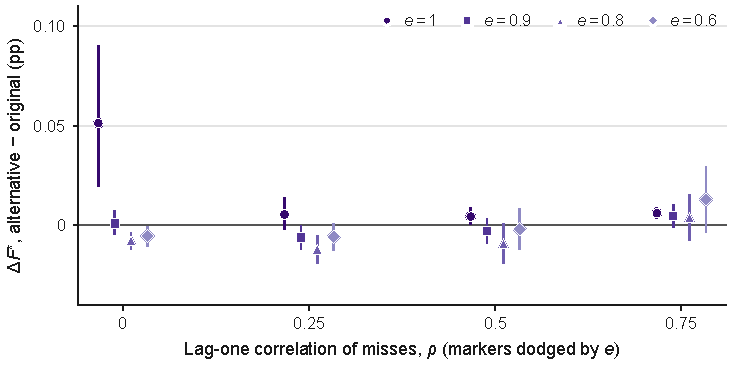
\includegraphics[width=.75\linewidth]{figures/fig_surface_diff.pdf}
\caption{Alternative minus original leading-order limit on the same 256 background seeds, completion .90$\to$.95, with paired whole-seed bootstrap 95\% intervals (20,000 draws; background Monte Carlo variation only); markers dodged by $e$. Every difference shown is below 0.06 percentage points; the largest of all 22 rows, $+0.27$, is at .95$\to$.99, $\rho=0$, $e=1$.}\label{fig:surface-diff}
\end{figure}

\begin{table}[htbp]\centering\footnotesize\setlength{\tabcolsep}{4pt}
\caption{The three prespecified predictions. Prediction 1 compares the alternative-workflow limit with the published rounded original value, as the protocol states; the paired difference from the exact same-seed original value and its whole-seed bootstrap 95\% interval are also shown. $\Delta$ values are percentage points.}\label{tab:predictions}
\begin{adjustbox}{max width=\linewidth}
\begin{tabular}{>{\raggedright\arraybackslash}p{.36\linewidth}rr>{\raggedright\arraybackslash}p{.24\linewidth}l}\toprule
Prediction & Reference & Result & Detail & Verdict\\\midrule
\tabinput{supplement_numbers/tab_predictions.tex}
\bottomrule\end{tabular}
\end{adjustbox}
\par\smallskip\raggedright The protocol reference .9235 is the exact root of the isolated two-opportunity crossing (.92353, Proposition~\ref{prop:interaction}). Prediction 3 used the protocol's two-point statistic, a linear interpolation between $e=.9$ and 1; its value is shown only as the record of this prediction. Because $\Delta(e)$ is strongly nonlinear in $e$, that statistic is not a location estimate: the fine-grid original-workflow crossing is .93361 (Section~\ref{sec:s-coef-extension}), also within .05 of .9235. No alternative-workflow fine grid was computed. The later estimate does not rescore these historical predictions.
\end{table}

\paragraph{Coefficient changes across workflows (post hoc).}
The alternative workflow lowered $K_0$ by 3.8--4.0\% in all 22 rows
(independent profile: $\mn3.9\%$ [$\mn6.8$, $\mn0.8$]) and $K_1$ by
3.8--4.0\% in 21 rows. The exception was a 10.2\% fall in $K_1$ at
.95$\to$.99, $\rho=0$, $e=1$, where prevention rose from 95.74\% to 96.01\%,
near the isolated two-opportunity value 96.0\%. Here $K_1$ is smallest, so the
loss of zero-opportunity bridges matters most. Such bridges contributed at most
0.3\% of original $K$; at $p=0$ they are hand bridges, not environmental routes.
None remained in the alternative workflow. The independent profile's per-seed
$K_1/K_0$ standard deviation fell from .0034 (range .2481--.2786) to .00003.
The survival-weighted opportunity mix otherwise changed little
(Table~\ref{tab:kmix}).

No ordered bridge history matched across workflows (0 of 256): same backgrounds
means same seeds, not same histories. Imported carriers averaged 9.20 versus
9.53 per observation window; patient-days averaged 1,640.4 versus 1,640.0.
Alternative windows averaged 4.92 relocations, 1.10 detected-patient-days waiting
in shared beds and no swaps. Per-worker independent $K_0$ changed by up to
2.6-fold, but role shares stayed close: nurses 86.7/86.1\%, physicians
10.6/11.0\% and radiography 2.7/2.9\%. Both banks agreed within .002 percentage
points in every primary limit in both workflows. Almost every surviving bridge
still crossed two opportunities, so redistribution changed the ratio little.
This explanation is post hoc. It does not establish invariance to bed management
in general: the leading term cannot see ungated environmental chains, and the
combined workflow change does not isolate either rule's effect. Differences in
finite-$p$ prevention therefore lie outside this leading term.

\begin{table}[htbp]\centering\footnotesize
\caption{Opportunity-count mix of the survival-weighted leading-order coefficient: percentage of mean $K$ contributed by bridges with $k$ intervening hygiene opportunities, primary profiles, same 256 backgrounds. Under the entry/exit rule every count between zones is even, so the columns are $k=0$, $k=2$ and $k\ge4$ (odd counts contribute 0). A $k=0$ bridge is a hand bridge with no intervening opportunity.}\label{tab:kmix}
\begin{adjustbox}{max width=\linewidth}
\begin{tabular}{llrrrrrr}\toprule
 & & \multicolumn{3}{c}{Original workflow} & \multicolumn{3}{c}{Alternative workflow}\\
\cmidrule(lr){3-5}\cmidrule(lr){6-8}
Profile & Arm & $k=0$ & $k=2$ & $k\ge4$ & $k=0$ & $k=2$ & $k\ge4$\\\midrule
\tabinput{supplement_numbers/tab_kmix.tex}
\bottomrule\end{tabular}
\end{adjustbox}
\end{table}

\paragraph{Finite-$p$ comparison (post hoc).}
All alternative-workflow fractions were within 1.4 points of their limits and
inside their 95\% intervals (Table~\ref{tab:posthoc}). In the original workflow,
the independent fraction was 7.6 points below its limit, or 8.4 after
common-baseline interpolation; the other profiles were within 2.3 points.
Yet $1000p^2\overline K_h/D^{(0)}$ explains only 31--60\% of alternative control
rates (25--57\% original), so higher-order absolute contributions are large.
They changed the alternative control and policy rates nearly proportionally;
this is an observed property, not a guarantee. Every interval also contains the
simpler two-opportunity comparator, so interval overlap cannot distinguish it
from the full leading-order limit. Finite-$p$ outcomes preceded this protocol.

\begin{table}[htbp]\centering\footnotesize\setlength{\tabcolsep}{4pt}
\caption{Post hoc, descriptive comparison of the alternative-workflow finite-$p$ results (512 paired seeds per profile, once-selected $p$) with the alternative-workflow leading-order limit, and leading-order versus measured absolute rates (per 1,000 patient-days; ratio in parentheses).}\label{tab:posthoc}
\begin{adjustbox}{max width=\linewidth}
\begin{tabular}{lrrrrrr}\toprule
Profile & Selected $p$ & \shortstack{Finite-$p$ $F$\\(\%) [95\%]} & \shortstack{Limit\\(\%)} & \shortstack{$F-$limit\\(pp)} & \shortstack{Control rate:\\leading / measured} & \shortstack{Policy rate:\\leading / measured}\\\midrule
\tabinput{supplement_numbers/tab_posthoc.tex}
\bottomrule\end{tabular}
\end{adjustbox}
\end{table}

\paragraph{Interpretation.} Agreement with finite-$p$ fractions is descriptive,
not validation: the fixed-horizon $p\to0$ limit has no finite-$p$ error bound.
Neither agreement nor the combined workflow comparison identifies either rule's
effect. Cross-platform reproducibility was checked only in original-workflow mode;
alternative coefficient records ran on macOS (Section~\ref{sec:s-repro}).

\subsection{Prespecified coefficient extension: crossing, policy definition and parameter grid}\label{sec:s-coef-extension}

\paragraph{Design.} The extension protocol specified 160 additional
profile-pair definitions: 14 crossing rows, 10 completion-range rows, four
transition-defined policy rows and a $11\times12$ parameter grid. Together with
22 archived pairs this gives 182 pairs on each of the same 256 original-workflow
background seeds. Duplicate parameter definitions were retained as numerical
checks. All backgrounds used the unchanged 30-bed model, 3\% admission carriage,
$p=0$, the care-zone entry/exit rule and 90 warmup plus 56 observation days.
Coefficient arms consume no random numbers and are fed the same event stream;
these rows are not independent new ICU histories.

For every seed the ordered event hash, three primary profiles, all 22 archived
pairs and duplicate pairs matched their archived references bitwise. All 256
records passed, none was excluded or replaced, and both benchmark seeds
reproduced their new arms on rerun. The 10-worker local batch used 54.89 measured
CPU-hours (55.03 whole-process CPU-hours), about 12\% above the 48.87 projected
by the 2-seed benchmark; the overrun, attributed to machine load, was reported
and not acted on. The 60-hour budget governed only the plan decision, which
used the projection. Disclosure: before launch, the implementer saw outcomes
on the 2 benchmark seeds while testing the summary script; the plan, protocol
and code did not change afterwards. Because coefficient Monte Carlo error is
small, those outputs were nearly as informative as the full study (post hoc):
over all 32,640 two-seed subsets of the 256 backgrounds, the standard deviation
of the .70$\to$.80, $e=.8$ clustering contrast was 0.02 points, and the two
benchmark seeds gave $+0.251$ points against $+0.254$ from all 256. The
protocol's precedence therefore rests on its file timestamp (01:57 EDT, before
the benchmark runs began at 02:19) and on its hash, first recorded at code
review (03:07); the protocol file was not under version control. The protocol, launch notes and reviewed code were preserved. The
original and independently implemented summaries agreed on the four prediction
decisions and numerical results. Point estimates are
$F^*=1-\operatorname{mean}(K_1)/\operatorname{mean}(K_0)$; intervals use 20,000
synchronous whole-seed bootstrap draws, with the declared seed 20261023.
They describe background Monte Carlo uncertainty only. Prediction decisions use
the prespecified point-estimate criteria, not multiplicity-adjusted tests.

\begin{table}[htbp]\centering\footnotesize
\caption{Four predictions declared before the coefficient extension, with criteria as written in the protocol. Failed predictions are retained. $D$ is the clustering contrast in percentage points; the crossing interval includes background Monte Carlo variability only.}\label{tab:extension-predictions}
\begin{tabular}{c>{\raggedright\arraybackslash}p{.40\linewidth}>{\raggedright\arraybackslash}p{.36\linewidth}l}\toprule
\# & Criterion & Observed & Decision\\\midrule
\tabinput{supplement_numbers/tab_extension_predictions.tex}
\bottomrule\end{tabular}
\end{table}

\paragraph{Crossing and completion ranges.} Prediction 1 held. All 20,000
draws had one crossing on the evaluated grid, between .93 and .94; linear
interpolation gives .93361 [.93358,.93365]. This supersedes the earlier two-point
location estimate, but interpolation error exceeds the bootstrap interval.
Near-root second differences are $-.30$ and $-.33$ points on the .01 grid;
concavity puts the linear root left of the smooth root. Post hoc quadratic,
cubic and quartic fits give .93379--.93382, outside the interval. On the isolated
bridge the same linear method misses the known root .92353 by
$2.2\times10^{-4}$ (estimate .92331), about three interval widths; a quadratic
misses by less than $2\times10^{-5}$. Thus about .934 is appropriate, and both
estimates satisfy Prediction 1.

Table~\ref{tab:extension-crossing} shows the nonlinear $\Delta(e)$, largest near
.8. The crossing is above the isolated root and near the renewal value .936.
Per-length roots (four opportunities: .845) do not bound a mixture's crossing:
the two arms weight bridge lengths differently (Table~\ref{tab:kmix}).

Prediction 2 failed in one of its eight components. At $e=.8$, the clustering
contrast for .70$\to$.80 was $+0.254$ percentage points, whereas the protocol
predicted $D<0$ (isolated bridge $\mn2.383$); its background interval was
[0.250, 0.258] points (Table~\ref{tab:extension-predictions} gives the bootstrap
draw count). The .60$\to$.70 contrast remained negative
($-0.935$ points), and the .80$\to$.90 contrast was positive ($+4.379$ points).
At perfect clearing the contrast remained negative at every tested range.
The risk this prediction took lay mainly in the three $e=.8$ signs, of which
two held: three of the five $e=1$ components (.80$\to$.90, .90$\to$.95 and
.95$\to$.99) used only archived pairs whose outcomes were known before the
protocol was written, and the two new $e=1$ components had isolated values of
$\mn13.4$ and $\mn17.1$ points. Post hoc and descriptively, in every range the ICU contrast exceeds the isolated two-opportunity value, by
0.66 to 5.29 points, so at $e=.8$ the full-coefficient reversal extends to
lower completion than the isolated bridge suggests: the sign change lies between
the .60$\to$.70 and .70$\to$.80 ranges, not between .70$\to$.80 and .80$\to$.90.
The isolated formula therefore does not determine every full-ICU sign, even
within the rare-transmission limit (Table~\ref{tab:extension-ranges}).

\begin{table}[htbp]\centering\footnotesize
\caption{Crossing scan: original-workflow $F^*$ (\%) at completion .90$\to$.95, and $\Delta=F^*(.5,e)-F^*(0,e)$ (percentage points). Brackets are whole-seed bootstrap 95\% intervals.}\label{tab:extension-crossing}
\begin{tabular}{rrrrl}\toprule
$e$ & $F^*(0,e)$ & $F^*(.5,e)$ & $\Delta$ & 95\% interval\\\midrule
\tabinput{supplement_numbers/tab_extension_crossing.tex}
\bottomrule\end{tabular}
\end{table}

\begin{table}[htbp]\centering\footnotesize
\caption{Completion-range contrasts in the original-workflow coefficient. Fractions are percentages; $\Delta$ and the isolated comparator are percentage points. All rows use the same 256 backgrounds. The isolated comparator has no Monte Carlo uncertainty.}\label{tab:extension-ranges}
\begin{adjustbox}{max width=\linewidth}
\begin{tabular}{lrrrrlr}\toprule
$h_0\to h_1$ & $e$ & $F^*(0,e)$ & $F^*(.5,e)$ & $\Delta$ & 95\% interval & Isolated $\Delta_2$\\\midrule
\tabinput{supplement_numbers/tab_extension_ranges.tex}
\bottomrule\end{tabular}
\end{adjustbox}
\end{table}

\paragraph{Transition-defined policy.} Direct-transition compliance of
90\%$\to$95\% requires per-boundary $.683772\to.776393$ at $\rho=0$ and
$.829180\to.908392$ at $\rho=.5$ (unrounded roots in computation).
Prediction 3 held: the perfect-clearing ICU contrast was 0.121 points, versus
$-21.5$ under the per-boundary policy (Table~\ref{tab:extension-transition}).
This was low-risk: its 5-point tolerance was about 40 times the observed contrast.
At $e=1$, matching transition compliance matches $q_2$, which carries $\rho$
in Proposition~\ref{prop:q12}; the isolated contrast is exactly zero.
The small ICU departure is new information. At $e=.8$ the ICU contrast remained
7.446 points, so matching transition compliance does not remove clustering
dependence with imperfect clearing.

The policies differ because their per-boundary completion levels differ by
profile. Forecasts depend on the chosen score; neither score is an artifact.
Boundary electronic monitoring and WHO direct observation measure different
units (Section~\ref{sec:s-hygiene}). This comparison assumes stationary Markov
completion and one exit and entry per direct move; it does not validate clinical
audit practice.

\begin{table}[htbp]\centering\footnotesize
\caption{Transition-defined 90\%$\to$95\% policy: original-workflow $F^*$ (\%), contrasting $\rho=.5$ with $\rho=0$. Each uses its own per-boundary completion levels. $\Delta$ and its 95\% interval are percentage points.}\label{tab:extension-transition}
\begin{tabular}{rrrrlr}\toprule
$e$ & $F^*(0,e)$ & $F^*(.5,e)$ & $\Delta$ & 95\% interval & Isolated $\Delta_2$\\\midrule
\tabinput{supplement_numbers/tab_extension_transition.tex}
\bottomrule\end{tabular}
\end{table}

\paragraph{Expanded renewal comparison.} Prediction 4 failed. On the 132-node
grid the maximum absolute discrepancy was 4.32 percentage points, exceeding
the predicted 3.5-point ceiling, at $\rho=.95,e=.5$. Post hoc and
descriptively, the renewal comparator exceeded $F^*$ at every node; 49 nodes
were within 0.5 points and 81 within 1 point; errors grow toward high $\rho$
and low $e$ (3.91 points at $\rho=.9$, $e=.5$); and for $\rho\le.7$, a cut
chosen after the failure was seen, the maximum was 2.48 points, at $\rho=.7$,
$e=.6$ (the grid has no $\rho=.75$ row). The historical 22-row maximum of 2.78 points remains correct on its
smaller domain. The complete expanded grid is given in
Table~\ref{tab:extension-grid}. These coefficients also supply the interpolated
measurement projection in Section~\ref{sec:s-uq}; no new per-opportunity
histogram was recorded for these non-primary arms. None of the extension tests
the sign reversal at finite $p$ or supplies a finite-$p$ error bound.

{\footnotesize
\begin{longtable}{rrrrrr}
\caption{Expanded original-workflow coefficient grid: completion .90$\to$.95, 256 background seeds. $F^*$ and $F_{\rm geo}$ are percentages; error is $F_{\rm geo}-F^*$ in percentage points. Intervals include background uncertainty only.}\label{tab:extension-grid}\\
\toprule
$\rho$ & $e$ & $F^*$ & 95\% interval & $F_{\rm geo}$ & Error\\\midrule\endfirsthead
$\rho$ & $e$ & $F^*$ & 95\% interval & $F_{\rm geo}$ & Error\\\midrule\endhead
\tabinput{supplement_numbers/tab_extension_fine_grid.tex}
\bottomrule
\end{longtable}
}


\section{Calibration, selection and baseline-matching checks}\label{sec:s-calibration}

\subsection{Selection procedures}\label{sec:s-selection}
Every study selected the transmission probability $p$ from baseline (control)
acquisitions only, then held it fixed for the paired policy comparison; policy
outcomes never selected $p$.
\begin{itemize}
\item \emph{Antecedent exploration}: 27 conditions with 64
paired seeds each (1,728 records). The rule took the lowest exact target hit,
otherwise the first increasing adjacent bracket, interpolating $p$ linearly
against pooled baseline rate, with no extrapolation or fallback. It selected
$p=.07602158$ (clustered misses) and $.07483996$ (imperfect clearing); its
independent grid had no point selection.
\item \emph{Independent-profile calibration grid}: 128 seeds at
$p=.13496571$, .15 and .165 gave baseline rates 2.311, 3.558 and 5.027 per 1,000
patient-days. The declared rule (exact hit, otherwise lowest increasing bracket
with linear interpolation of $p$ against rate; fixed $p=.15$ fallback recorded as
a failure) selected $p=.14327559$ from the first bracket. The calibration
validity check passed.
\item \emph{Original holdout}: the three probabilities were frozen and
evaluated on 512 fresh paired seeds per profile.
\item \emph{Opportunity-rule follow-up} and
\emph{alternative-workflow study} used their own declared
rules (Sections~\ref{sec:s-clock} and~\ref{sec:s-alt-selection}). The
alternative study interpolated on the log--log scale; the original rules were
linear in $p$ versus rate (or versus acquisition count in earlier refinement
and validation rules). None of the original rules was logarithmic.
\end{itemize}

\subsection{All baseline-matching and target-band checks}\label{sec:s-gates}
The original holdout study declared six simultaneous 99.167\% interval checks:
each profile's baseline rate interval had to lie wholly inside [2.7, 3.3] per
1,000 patient-days, and each pairwise baseline-rate-ratio interval wholly inside
$[1/1.1, 1.1]$. These are declared numerical tolerances, not tests of exact
equality; any failed check prevents a matched-baseline claim, and passing
depends on both precision and the underlying rates. All six failed, although
the calibration validity check passed. The opportunity-rule follow-up added two
target checks (entire 99.167\% interval inside [2.7, 3.3]); both failed. These
are the eight failed checks. The alternative-workflow study used descriptive
95\% band checks; the clustered and imperfect checks failed. No refitting or
sample extension was made in response to any failure. The coarse
inherited-clock sweep also found no sampled match (Section~\ref{sec:s-clock}).

\begin{table}[htbp]\centering\footnotesize\setlength{\tabcolsep}{4pt}
\caption{Every baseline-matching and target-band check, with verbatim estimates and intervals (rates per 1,000 patient-days).}\label{tab:gates}
\begin{adjustbox}{max width=\linewidth}
\begin{tabular}{rllrrll}\toprule
\# & Study & Check & Estimate & Interval & Allowed band & Outcome\\\midrule
\multicolumn{7}{l}{\emph{Original holdout: six simultaneous 99.167\% interval checks (200,000 whole-seed draws)}}\\
\tabinput{supplement_numbers/tab_gates_original.tex}
\multicolumn{7}{l}{\emph{Opportunity-rule follow-up: selected inherited-clock target checks (99.167\% family level)}}\\
7 & Clock follow-up & Clustered baseline rate & 3.09 & [2.85, 3.33] & [2.7, 3.3] & Not met\\
8 & Clock follow-up & Imperfect baseline rate & 2.85 & [2.62, 3.09] & [2.7, 3.3] & Not met\\
\bottomrule\end{tabular}
\end{adjustbox}

\medskip
\begin{adjustbox}{max width=\linewidth}
\begin{tabular}{lrrl}\toprule
\multicolumn{4}{l}{\emph{Alternative-workflow study: descriptive 95\% target-band checks, band [2.7, 3.3]}}\\
Profile & Baseline rate & 95\% interval & Interval in band?\\\midrule
\tabinput{supplement_numbers/tab_gates_alt.tex}
\bottomrule\end{tabular}
\end{adjustbox}
\end{table}

\subsection{Selection uncertainty}\label{sec:s-selection-uncertainty}
Retrospective bootstraps of the saved calibration grids describe how variable
the selected $p$ would have been. They condition on the already chosen grids and
exclude uncertainty from grid choice and interpolation error; they were not
propagated into the policy intervals (Section~\ref{sec:s-selprop} gives an
approximate propagation).

{\footnotesize\setlength{\tabcolsep}{3pt}
\begin{longtable}{p{.065\linewidth}p{.06\linewidth}p{.225\linewidth}p{.225\linewidth}p{.11\linewidth}p{.075\linewidth}p{.13\linewidth}}
\caption{Independent-profile selection uncertainty from the three-probability baseline grid (50,000 draws, seed 20261010). Conditional intervals retain only exact-hit/increasing-bracket selections; fallback-inclusive intervals apply the fixed $p=.15$ fallback and retain failures. Selection diagnostics, not propagated holdout uncertainty.}\label{tab:sel-independent}\\
\toprule
Cohort & Seeds & Selected $p$ [conditional 95\%] & $p$ [fallback-inclusive 95\%] & Failed draws & Failure (\%) & Nonmonotone\\
\midrule\endfirsthead
Cohort & Seeds & Selected $p$ [conditional 95\%] & $p$ [fallback-inclusive 95\%] & Failed draws & Failure (\%) & Nonmonotone\\
\midrule\endhead
pooled & 128 & 0.14328 [0.14004, 0.14792] & 0.14328 [0.14004, 0.14792] & 0 / 50000 & 0.00\% & 0\\
A & 64 & 0.14301 [0.13739, 0.15084] & 0.14301 [0.13741, 0.15083] & 740 / 50000 & 1.48\% & 200\\
B & 64 & 0.14343 [0.13967, 0.14984] & 0.14343 [0.13967, 0.14984] & 0 / 50000 & 0.00\% & 112\\
\bottomrule
\end{longtable}

\begin{longtable}{>{\raggedright\arraybackslash}p{.18\linewidth}>{\raggedright\arraybackslash}p{.12\linewidth}>{\raggedright\arraybackslash}p{.11\linewidth}>{\raggedright\arraybackslash}p{.21\linewidth}>{\raggedright\arraybackslash}p{.11\linewidth}>{\raggedright\arraybackslash}p{.14\linewidth}}
\caption{Retrospective uncertainty in the antecedent 27-condition exploratory selection (50,000 joint whole-seed draws, seed 20261011). Each pooled analysis has 64 seeds; historical local and cluster subsets have 32 each, and the stratified diagnostic resamples 32 from each. Intervals condition on defined selections; any failed draw makes the unconditional interval unavailable.}\label{tab:sel-exploratory}\\
\toprule
Profile & Cohort & Point $p$ & Conditional 95\% interval & Failed draws & Unconditional\\
\midrule\endfirsthead
Profile & Cohort & Point $p$ & Conditional 95\% interval & Failed draws & Unconditional\\
\midrule\endhead
Independent & pooled64 & undefined & [0.13179, 0.13496] & 49,522 & unavailable\\
Clustered misses & pooled64 & 0.07602 & [0.07346, 0.07873] & 0 & as conditional\\
Imperfect clearing & pooled64 & 0.07484 & [0.07243, 0.07785] & 0 & as conditional\\
Independent & local32 & undefined & [0.13181, 0.13484] & 49,721 & unavailable\\
Clustered misses & local32 & 0.07693 & [0.07342, 0.08058] & 7 & unavailable\\
Imperfect clearing & local32 & 0.07556 & [0.07206, 0.08087] & 358 & unavailable\\
Independent & cluster32 & undefined & [0.12829, 0.13485] & 44,158 & unavailable\\
Clustered misses & cluster32 & 0.07497 & [0.07097, 0.07942] & 13 & unavailable\\
Imperfect clearing & cluster32 & 0.07418 & [0.07072, 0.07789] & 3 & unavailable\\
Independent & 32+32 & undefined & [0.13196, 0.13496] & 49,491 & unavailable\\
Clustered misses & 32+32 & 0.07602 & [0.07350, 0.07869] & 0 & as conditional\\
Imperfect clearing & 32+32 & 0.07484 & [0.07239, 0.07785] & 1 & unavailable\\
\bottomrule\end{longtable}
}
The bank-A independent conditional interval uses 49,260 valid draws; its 740
failed draws remain visible. The old independent exploratory grid has no point
selection despite occasional defined bootstrap draws. The original 20,000-draw
exploratory result was reconstructed before extension to 50,000 draws, and all
1,536 holdout and 1,728 exploratory record hashes were verified unchanged. No
conclusion about the cause of the baseline undershoot follows from linear
interpolation alone.

\subsection{Baseline-mismatch elasticity and implied bias}\label{sec:s-bias}
\paragraph{Baseline-mismatch estimator.} Seed-paired original-workflow
conditions varying $p$ estimate $\beta_B=\mathrm dF/\mathrm d\ln B$, in
percentage points per natural-log baseline (Table~\ref{tab:slope-inputs}).
A 10\% baseline increase changes $F$ by
$\ln(1.1)\beta_B\approx0.095\beta_B$; estimated bias relative to 3.0 is
$F(B_{\mathrm{obs}})-F(3.0)\approx\beta_B\ln(B_{\mathrm{obs}}/3)$.
Positive bias means observed $F$ exceeds its estimated value at 3.0.

Intervals use 20,000 whole-seed percentile draws (seed 20261021), preserving
shared seeds within banks. Four 128-seed holdout strata preserve overlap with
the independent upper bank. Recomputed intervals differ from the archived
200,000-draw values by at most .12 points; point values agree.
Independent numerical verification and rounding differences are documented in
the repository execution records.

{\footnotesize\setlength{\tabcolsep}{3pt}
\begin{longtable}{>{\raggedright\arraybackslash}p{.2\linewidth}>{\raggedright\arraybackslash}p{.22\linewidth}rrrr}
\caption{Original-workflow conditions used for the slopes (care-zone opportunities, completion .90 vs .95). Control rate per 1,000 patient-days and $F$ (\%) with 95\% intervals. Conditions in the same bank share seeds.}\label{tab:slope-inputs}\\
\toprule
Condition & Seed bank & Seeds & $p$ & Control rate $B$ [95\%] & $F$ (\%) [95\%]\\\midrule\endfirsthead
Condition & Seed bank & Seeds & $p$ & Control rate $B$ [95\%] & $F$ (\%) [95\%]\\\midrule\endhead
\tabinput{supplement_numbers/tab_slope_inputs.tex}
\bottomrule
\end{longtable}

\begin{table}[htbp]\centering\footnotesize\setlength{\tabcolsep}{3pt}
\caption{Slopes. $\beta_B=\mathrm dF/\mathrm d\ln B$ and $\mathrm dF/\mathrm d\ln p$ in percentage points; $\gamma=\mathrm d\ln B/\mathrm d\ln p$. Two-point slopes are paired finite differences; OLS slopes are equal-weight three-point fits. Every $\beta_B$ interval includes zero.}\label{tab:slopes}
\begin{adjustbox}{max width=\linewidth}
\begin{tabular}{llrrrrr}\toprule
Profile & Segment & Baselines & $\beta_B$ [95\%] & Per +10\% baseline [95\%] & $\mathrm dF/\mathrm d\ln p$ [95\%] & $\gamma$ [95\%]\\\midrule
\tabinput{supplement_numbers/tab_slopes.tex}
\bottomrule\end{tabular}
\end{adjustbox}
\end{table}
}
The center-to-1.25$\times$center segment is the primary slope because it is the
only segment whose baselines bracket 3.0 for every profile. The independent
primary segment spans a 2.6-fold baseline range (2.78 to 7.29), and the
environmental full-model segments below the target have the opposite point
sign, so local linearity is weakest for that profile, although its observed
shortfalls are the smallest. The independent primary slope equals the
upper-minus-matched-center contrast of the opportunity-rule study ($+4.7$
percentage points, Table~\ref{tab:rule-contrasts}) divided by its log-baseline
span. Applying the primary slopes from the center to 3.0 reproduces the
common-baseline $F_{\mathrm{cb}}$ of Section~\ref{sec:s-common} to within 0.027 percentage
points.

Two local estimators are reported. \emph{Piecewise} uses the low-to-center slope
for any part of the span below the sensitivity center and the center-to-high
slope above it; \emph{primary} uses the center-to-high slope throughout. Their
point estimates coincide when the observed baseline lies above the sensitivity
center. Joint intervals resample the slope and the observed baseline together.

\begin{table}[htbp]\centering\scriptsize\setlength{\tabcolsep}{2.5pt}
\caption{Implied bias $F(B_{\mathrm{obs}})-F(3.0)$ in percentage points with joint 95\% intervals, the range of point estimates across every slope estimator in Table~\ref{tab:slopes}, and $F$ adjusted to 3.0 with the piecewise estimator. Alternative-workflow rows reuse original-workflow slopes (a transfer assumption).}\label{tab:bias}
\begin{adjustbox}{max width=\linewidth}
\begin{tabular}{llrrrrrrr}\toprule
Workflow & Profile & $B_{\mathrm{obs}}$ & vs 3.0 & Bias, piecewise [95\%] & Bias, primary [95\%] & Range, all estimators & $F$ obs.\ (\%) & $F$ at 3.0 (\%) [95\%]\\\midrule
\tabinput{supplement_numbers/tab_bias.tex}
\bottomrule\end{tabular}
\end{adjustbox}
\end{table}

\begin{table}[htbp]\centering\footnotesize\setlength{\tabcolsep}{3pt}
\caption{Implied bias in the prespecified contrasts (percentage points). Observed-contrast intervals are recomputed here so they can be combined draw by draw and differ slightly from the archived intervals (different stream and stratification); the archived intervals remain authoritative. Adjusted contrasts are post hoc and descriptive.}\label{tab:contrast-bias}
\begin{adjustbox}{max width=\linewidth}
\begin{tabular}{llrrrr}\toprule
Workflow & Contrast & Observed [98.333\%] & Bias, piecewise [95\%] & Bias, primary [95\%] & Adjusted to 3.0 [98.333\%]\\\midrule
\tabinput{supplement_numbers/tab_contrast_bias.tex}
\bottomrule\end{tabular}
\end{adjustbox}
\end{table}

\paragraph{Results and assumptions.} Estimated bias is at most .52 points
under the two local estimators (joint 95\% intervals within $[\mn2.13,2.13]$),
or .98 using any tested slope. Estimated contrast bias is at most .89 points
(intervals within $[\mn2.34,3.27]$); all six adjusted contrasts still exclude
zero at 98.333\%. For scale, Monte Carlo half-widths are 2.30--5.24 points
and declared contrasts 11.7--49.2 points. Every slope interval includes zero,
so neither direction nor curvature is resolved.

These post hoc adjustments assume local linearity in $\ln B$ and that changing
$p$ represents the relevant baseline correction. Seed, workflow or admission-mix
differences need not have that response. Alternative-workflow results transfer
original slopes because no alternative sensitivity bank exists; its grid checks
only $\gamma$. Separate environmental-bank points (baselines .40--2.29;
512 seeds) supply secondary slopes only. Intervals omit interpolation-model,
structural and clinical-input uncertainty; the estimates are not error bounds
and cannot turn failed checks into passes. Adjusted 512-seed holdout fractions
differ from 256-seed common-baseline estimates because their center samples
differ (66.3/55.3/29.8\% versus 67.6/55.9/27.0\% at the same $p$).

\subsection{Propagating selection uncertainty}\label{sec:s-selprop}
Each workflow selected $p$ once. The implied shift in $F$ from moving $p$ to an
end of its conditional 95\% selection interval is
$\mathrm dF/\mathrm d\ln p\times\ln(p_{\mathrm{bound}}/p_{\mathrm{selected}})$,
using the primary slope (for the alternative workflow, the original-workflow
slope). ``With slope uncertainty'' is a per-draw envelope: for each bootstrap
draw of the slope the smaller and larger of the two endpoint shifts are taken,
and the table reports the 2.5th percentile of the smaller and the 97.5th
percentile of the larger. The Monte Carlo half-width is half the width of the
archived, unrounded 95\% interval of $F$. The combined half-width
$\sqrt{\mathrm{MC}^2+S^2}$ uses $S$, the largest absolute shift over the slope's
point value and 95\% endpoints at the two ends of the $p$ interval; it treats the
two sources as independent and symmetric and is descriptive only.

\begin{table}[htbp]\centering\footnotesize\setlength{\tabcolsep}{3pt}
\caption{Selection uncertainty in $p$ propagated to $F$ (percentage points). Original selected-$p$ intervals: independent from Table~\ref{tab:sel-independent} (pooled row); clustered and imperfect from Table~\ref{tab:sel-exploratory} (pooled64 rows, older 64-seed design). Alternative intervals: Table~\ref{tab:alt-grid}. All have 0 failed draws.}\label{tab:selprop}
\begin{adjustbox}{max width=\linewidth}
\begin{tabular}{ll>{\raggedright\arraybackslash}p{2.75cm}r>{\raggedright\arraybackslash}p{2.0cm}rrrr}\toprule
Workflow & Profile & Selected $p$ [95\%] & \shortstack{Interval\\vs $p$} & $\mathrm dF/\mathrm d\ln p$ [95\%] & \shortstack{Shift,\\point slope} & \shortstack{Shift, slope\\envelope} & \shortstack{MC\\half-width} & Combined\\\midrule
\tabinput{supplement_numbers/tab_selection_prop.tex}
\bottomrule\end{tabular}
\end{adjustbox}
\end{table}

Selection uncertainty moves $F$ by at most 0.67 percentage points at the point
slope, or 2.12 points allowing for slope uncertainty; slope uncertainty,
not the width of the $p$ interval, dominates the wider bound. Imperfect clearing
in the alternative workflow chose the lower bracket in 2,861 of 20,000 selection
draws, and its archived interval includes those draws. As a sensitivity check
for the transfer assumption, the baseline-on-$p$ part can be replaced by the
alternative grid's own log--log slope over the m1--m2 bracket
(Table~\ref{tab:selprop-alt}); the point shifts stay below 0.5 percentage points.

\begin{table}[htbp]\centering\footnotesize\setlength{\tabcolsep}{3pt}
\caption{Alternative-workflow sensitivity: original-workflow $\beta_B$ combined with the alternative grid's own $\gamma$ over the m1--m2 bracket.}\label{tab:selprop-alt}
\begin{adjustbox}{max width=\linewidth}
\begin{tabular}{lrrrrr}\toprule
Profile & Alternative grid $B$, m1 to m2 & Alternative $\gamma$ [95\%] & Original $\gamma$ & $\mathrm dF/\mathrm d\ln p$ [95\%] & Shift, point slope\\\midrule
\tabinput{supplement_numbers/tab_selection_altgamma.tex}
\bottomrule\end{tabular}
\end{adjustbox}
\end{table}

\section{Common-baseline post hoc interpolation}\label{sec:s-common}
\paragraph{Design.} After all eight matching checks and the bracketing outcomes
were known, a secondary analysis of existing original-workflow records was
declared; its protocol preceded the new bootstrap calculations. For each profile
the lower condition is its fixed center probability and the upper condition is
1.25 times that probability. The independent comparison uses the 256 matched
holdout/upper seeds; clustered misses and imperfect clearing use the 256
sensitivity seeds. No simulation was run at the interpolated probability.

\paragraph{Estimator.} With pooled control and policy rates $B_\ell,B_u$ and
$P_\ell,P_u$ at $p_\ell,p_u$, and each log rate assumed locally linear in
$\log p$,
\begin{equation}
w=\frac{\log 3-\log B_\ell}{\log B_u-\log B_\ell},\qquad
p^*=p_\ell^{1-w}p_u^{w},\qquad
F_{\mathrm{cb}}=1-\frac{P_\ell^{1-w}P_u^{w}}{3}.
\end{equation}
The interpolated baseline equals 3 by construction; this standardization does not
test whether the simulator attains that rate at $p^*$. Whole seeds were
resampled within banks A and B (128 each), 50,000 draws, seed 20261016; shared
seed lists were resampled synchronously across conditions, and the independent
and sensitivity lists independently. Rates, $w$ and $F_{\mathrm{cb}}$ were recomputed from
pooled counts and patient-days in each draw. The intervals cover Monte Carlo
uncertainty conditional on the input probabilities and the interpolation rule;
they exclude interpolation error, original probability selection, structural
uncertainty and clinical-input uncertainty.

\begin{table}[htbp]\centering\footnotesize
\caption{Post hoc common-baseline estimates (256 seed-matched pairs at each bracketing probability per profile). Target 3.0 is imposed by interpolation, not verified by new simulation. The absolute decrease equals $3F_{\mathrm{cb}}$, not an observed count difference at $p^*$. The original 512-pair count benefits remain 3.13, 2.46 and 1.24 acquisitions prevented per 56-day run at the original probabilities.}\label{tab:common}
\begin{adjustbox}{max width=\linewidth}
\begin{tabular}{lrrrr}\toprule
Profile & Baseline bracket & Implied $p^*$ & Prevention (\%) [95\%] & Absolute decrease [95\%]\\\midrule
Independent misses & 2.777--7.289 & 0.145853 & 66.7 [62.1, 71.2] & 2.00 [1.86, 2.14]\\
Clustered misses & 2.630--5.029 & 0.079545 & 55.0 [50.7, 59.4] & 1.65 [1.52, 1.78]\\
Imperfect clearing & 2.809--5.928 & 0.076328 & 30.0 [23.6, 36.6] & 0.90 [0.71, 1.10]\\
\bottomrule\end{tabular}
\end{adjustbox}
\end{table}

The three contrasts were 11.7 [4.0, 19.2] (independent minus clustered), 36.7
[26.8, 46.2] (independent minus imperfect) and 25.0 [15.3, 34.5] (clustered minus
imperfect) percentage points; these are Bonferroni-adjusted 98.333\% percentile
bootstrap intervals within this secondary family of three, not tests of actual
baseline equivalence. The target lay outside the resampled bracket, so the
estimator extrapolated, in 2,267 (4.534\%), 21 (0.042\%) and 1,922 (3.844\%) of
50,000 draws; extrapolating draws were retained and no draw was undefined.

\paragraph{Descriptive checks.} Arithmetic instead of logarithmic interpolation
shifts $F_{\mathrm{cb}}$ by at most 0.03 percentage points. Three-point curvature shifts the
clustered and imperfect estimates by $\mn0.21$ and $\mn0.07$ points (the
independent profile has no third matched condition). Using the full 512-seed
lower conditions gives 67.8\% [64.8, 70.8], 55.5\% [52.3, 58.7] and 27.5\% [23.0,
32.0]; these intervals were corrected after review to preserve the overlap
between the independent upper seeds and the lower bank (a dated amendment is
archived; the primary analysis is unchanged). At a target of 2.7, 72.0\% of
independent and 84.1\% of imperfect draws extrapolate, so that check cannot be
presented as interpolation throughout the target band. A review-requested
Linux-only subset of 192 independent pairs gave 66.6\% [61.3, 72.0], with 18.8\%
of draws extrapolating; this changes the seed subset as well as the platform
mixture and does not establish platform equivalence
(Section~\ref{sec:s-stability}). These checks do not bound interpolation or
model error.

\paragraph{Verification.} Independent implementations checked the points and
intervals; the later raw-data reimplementation was not blind. Numerical
agreement does not convert any failed matching check into a pass. Detailed
comparison tolerances and record checks are in the execution records.

\section{Alternative-workflow study}\label{sec:s-alternative}

\subsection{Protocol}\label{sec:s-alt-protocol}
The protocol preceded this study's outcomes, with original-workflow
results and limitations already known; it is prospective for its own outputs,
not for the earlier results. It asked whether the disagreement among the three
hygiene profiles persists when every bedside site is cleared as its patient
leaves (discharge or relocation) and detected carriers move only into empty
isolation beds (Table~\ref{tab:workflows}). If no isolation bed is empty the
carrier stays in its shared bed with that bed's multiplier; there are no
occupant swaps and no added contact-precaution effect. Site clearing removes
contamination and its origin label without resetting the daily cleaning clock;
initial admission to a never-occupied bed adds no cleaning event. All other
source, admission, staffing, transfer, hygiene and timing rules are inherited.
The rules apply in warmup and observation. This is one combined alternative
world: the design cannot attribute any change to vacancy cleaning or to the
isolation rule separately, and original-versus-alternative results are
descriptive structural sensitivity, not an isolated causal effect.

\emph{Fixed workload and selection.} The baseline grid used 0.5, 1, 2 and 4 times
each profile's original probability with 128 shared fresh seeds (1,536 baseline
records; 90 warmup and 56 observation days at completion .90). Each probability
was selected once from pooled baseline acquisitions per 1,000 patient-days,
target 3: the lowest-$p$ exact hit, otherwise the lowest-$p$ adjacent increasing
bracket with both rates positive, interpolating $\log$ rate linearly in $\log p$.
No extrapolation, pseudocount, alternative interpolator, fallback, grid
expansion or use of policy outcomes was allowed. After grid validation the
selection and derived policy configuration were hash-bound to the freeze and to
every baseline record. Each profile then received 512 fresh paired control/policy
seeds, shared across profiles and disjoint from the grid seeds; state was cloned
after warmup and completion was .90 versus .95 with memory retained. The
scientific ceiling was 3,072 records and was used exactly.

\emph{Inference.} Pooled rates, $F$, absolute rate change and mean acquisitions
prevented; 20,000 synchronous whole-seed bootstrap draws (seed 20261017; grid and
policy streams from NumPy seed sequences with entropy [20261017, 0] and
[20261017, 1]); 98.333\% intervals for the fixed three-contrast
Bonferroni family and descriptive 95\% intervals otherwise. Baseline 95\%
intervals were checked against the band [2.7, 3.3] as a descriptive target-band
check, not a profile-equivalence test, with no refitting or added seeds allowed.
Policy intervals condition on the once-selected $p$; they do not propagate
selection uncertainty or interpolation-model error.

\subsection{Selection}\label{sec:s-alt-selection}
\begin{table}[htbp]\centering\footnotesize\setlength{\tabcolsep}{3.5pt}
\caption{Alternative-workflow baseline grid (128 seeds per point): acquisitions per 1,000 patient-days (acquisition counts in parentheses) at $m\times$ the original probability, and the once-selected probability. Every profile used the lowest positive increasing adjacent bracket (m1--m2) with log--log interpolation; there were no exact hits, nonincreasing segments or zero lower rates. The selection bootstrap (20,000 draws) had no failed or undefined draws; the last column counts draws that selected the lower (m0.5--m1) bracket.}\label{tab:alt-grid}
\begin{adjustbox}{max width=\linewidth}
\begin{tabular}{lrrrrrrr}\toprule
Profile & m0.5 & m1 & m2 & m4 & Selected $p$ ($\times$m1) & Conditional 95\% & Lower-bracket draws\\\midrule
Independent & 0.205 (43) & 1.919 (403) & 17.03 (3,574) & 96.73 (20,303) & 0.165111 (1.152) & [0.15999, 0.17033] & 0\\
Clustered misses & 0.433 (91) & 2.463 (517) & 25.15 (5,280) & 161.72 (33,952) & 0.080633 (1.061) & [0.07801, 0.08332] & 7\\
Imperfect clearing & 0.538 (113) & 2.828 (594) & 30.07 (6,312) & 168.58 (35,387) & 0.076144 (1.017) & [0.07338, 0.07862] & 2,861\\
\bottomrule\end{tabular}
\end{adjustbox}
\end{table}
Imperfect clearing chose the lower bracket in 14.3\% of selection draws, yet its
conditional $p$ interval is still narrow (about $\pm$3.5\%). The selected $p$
values are defined to within 1 to 4 units in the last place, depending on the
summation order of patient-days; all 1,536 policy records use the cluster's $p$
exactly.

\subsection{Results}\label{sec:s-alt-results}
\begin{table}[htbp]\centering\scriptsize\setlength{\tabcolsep}{2.5pt}
\caption{Holdout results in the two workflows (512 paired seeds per profile and workflow). Rates per 1,000 patient-days in the 56-day observation window; acquisitions are pooled control$\to$policy counts; mean prevented is acquisitions prevented per 56-day ICU run. Descriptive 95\% intervals; original-workflow intervals use 200,000 whole-seed draws, alternative-workflow intervals 20,000. The two studies differ in rules, selected $p$, seeds and execution; the side-by-side display is context only and defines no between-workflow estimand.}\label{tab:holdout-both}
\begin{adjustbox}{max width=\linewidth}
\begin{tabular}{llrrrrrrr}\toprule
Profile & Workflow & $p$ & Control rate & Policy rate & Acquisitions & $F$ (\%) & Rate reduction & Mean prevented\\\midrule
\tabinput{supplement_numbers/tab_holdout_both.tex}
\bottomrule\end{tabular}
\end{adjustbox}
\end{table}

\begin{table}[htbp]\centering\footnotesize
\caption{Prespecified between-profile contrasts in $F$ (percentage points) with 98.333\% intervals (fixed three-contrast Bonferroni families, one per study). Contrasts compare fixed configurations whose baselines differ; they are not contrasts at a common baseline. No original-versus-alternative difference is an estimand.}\label{tab:contrasts-both}
\begin{adjustbox}{max width=\linewidth}
\begin{tabular}{lrr}\toprule
Contrast & Original workflow [98.333\%] & Alternative workflow [98.333\%]\\\midrule
\tabinput{supplement_numbers/tab_contrasts_both.tex}
\bottomrule\end{tabular}
\end{adjustbox}
\end{table}

All three alternative-workflow contrasts exclude zero at 98.333\%, ordering
independent $>$ clustered $>$ imperfect (Tables~\ref{tab:holdout-both}
and~\ref{tab:contrasts-both}); no bootstrap statistic was undefined.
Only the independent baseline passed the descriptive target-band check.
Clustered and imperfect baselines were below 2.7 and happened to differ by less
than .005; they were not matched. Results condition on selected $p$.

The 128-seed m1 grid estimates were imprecise and overdispersed
(variance/mean about 1.9): 2.46 [2.18,2.77] for clustering and
2.83 [2.51,3.15] for imperfect clearing. The latter selected $p$ was only 1.7\%
above m1, but its holdout baseline was 2.63, suggesting an upward grid fluctuation.
For clustering, grid error cannot be separated from curvature (log--log slopes
2.5 below and 3.35 above m1). Neither source enters policy intervals;
Section~\ref{sec:s-bias} estimates the implied bias under stated assumptions.

\emph{Workflow counters.} Mean per 56-day record (control / policy): isolation
relocations (equal to relocation clears) 6.74 / 5.29, 6.62 / 5.80 and 6.70 / 6.21
in the three profiles; detected-patient-days spent waiting in a shared bed
because no isolation bed was empty 1.68 / 1.25, 1.68 / 1.42 and 1.81 / 1.58
(per-tick counter divided by 2,592 ticks per day; it counts patient-ticks, not
patients); discharge clears that removed contamination 5.90 / 4.31, 2.31 / 1.75
and 2.22 / 1.88; relocation clears that removed contamination 2.52 / 1.63,
1.08 / 0.70 and 1.03 / 0.81; contaminated vacancy clears were 6.2--8.1\% of
depositions. Discharge clears equalled discharges (about 311 per record), no
occupied destination was ever attempted, and scheduled clears were 1,680 in
every record. The waiting time, about 1\% of colonized patient-days and 0.1\% of
all patient-days, bounds how often the background differs from the original
workflow, not how much $K$ differs; Section~\ref{sec:s-coef-alt} reports the
directly computed coefficient.

\emph{Face-validity and resources (post hoc).} Table~\ref{tab:face} gives
alternative control quantities. Site contamination differs about threefold
at similar acquisition baselines, suggesting positivity could constrain $p$
separately from the hygiene law. A reported 2.1\% environmental positivity
\citep{wei2021} offers face validity only: organisms, sampling and binary sites
differ. About 17,000 extra completions per run give threefold different returns
per acquisition prevented. Natural contamination episodes recover stationary
$q_1,q_2$ here because pickups are independent of completion state and
contamination does not change behaviour. Episode-selection bias remains a
real-world concern.

\begin{table}[htbp]\centering\footnotesize
\caption{Descriptive face-validity and resource quantities, alternative-workflow control arms (512 records per profile, 56-day observation window; descriptive, no intervals). Natural-episode survival: survived over at-risk counts at the first and second opportunity after pickup, stationary values in parentheses.}\label{tab:face}
\begin{adjustbox}{max width=\linewidth}
\begin{tabular}{lrrr}\toprule
Quantity & Independent & Clustered & Imperfect\\\midrule
\tabinput{supplement_numbers/tab_face_validity.tex}
\bottomrule\end{tabular}
\end{adjustbox}
\end{table}

\subsection{Verification}\label{sec:s-alt-verification}
Production selection and analysis used the pinned Linux runtime. Post-collection
checks are summarized in Table~\ref{tab:alt-verif}; exact receipts and comparison
tolerances are in the repository execution records. These are internal
automated and delegated checks, not external peer review.
\begin{table}[htbp]\centering\small
\caption{Post-collection checks of the alternative workflow.}\label{tab:alt-verif}
\begin{tabular}{p{.24\linewidth}p{.67\linewidth}}\toprule
Check & Finding\\\midrule
Inputs and records & Transport and frozen-input hashes agreed; all 1,536 grid records and 1,536 policy pairs passed completeness, counter and route checks.\\
Selection and analysis & Cross-platform frozen-code recomputation was bitwise; independent estimates agreed to numerical precision.\\
Runtime limitation & The unmodified frozen analyzer refused the local runtime. Cross-platform checks evaluated, but did not enforce, its pins; no second exact-runtime analysis followed collection.\\
Simulation recomputation & Five of 3,072 production records were re-simulated on macOS and agreed after runtime fields were removed.\\
\bottomrule\end{tabular}
\end{table}

\subsection{Execution limitations}\label{sec:s-alt-provenance}
A pre-production executable-identity failure produced no scientific records.
A documented amendment changed runtime and provenance checks, leaving scientific
functions unchanged, before the first record. All production records then used
one Linux compute host and pinned package set. The amendment review was not
blind. Seed-disjointness checks covered locally archived prior studies only;
banks held only on the cluster were not checked. Absence of restarts was inferred
from saved files because terminal scheduler accounting was not collected.
Execution details are retained in the repository.

\subsection{Attribution limits}\label{sec:s-alt-limits}
No original-versus-alternative difference has a declared estimand or interval.
This includes the independent $F$ (67.6\% versus 76.5\%), the
independent-minus-clustered contrast (11.7 versus 22.8 percentage points), the
selected probabilities (15\%, 6\% and 2\% higher), the lower baseline at the
original probability (independent grid m1 1.92 [1.70, 2.15] against the original
holdout's 2.83 [2.66, 3.01]) and the near-disappearance of carry-over labels
(Section~\ref{sec:s-routes}). Each mixes two rule changes, a different selected
$p$, fresh seeds and a separate study, so none is described as having grown,
shrunk or been removed. The two rules are also entangled: with swaps a
relocation never leaves a bed vacant, so separating them factorially would
require an extra rule such as cleaning at swap. What follows from the model's
rules rather than from estimated effects is that vacancy cleaning removes
pre-admission contamination except deposits made while a bed is empty, that
vacancy cleaning cannot change the $p=0$ coefficient, and that the isolation
rule can. The alternative workflow is one illustrative combination of rules,
not a clinical practice and not a family of workflows.

\section{Route labels in both workflows}\label{sec:s-routes}
\paragraph{Labels.} Passive histograms record, for every acquired colonization,
the pickup that began the infecting hand's current uncleared contamination
episode and the number of hygiene opportunities between that pickup and the
transfer. Individual event traces were not saved. Four labels are
used: \emph{patient pickup}; \emph{own-zone site, current stay} (pickup from the
patient's own bedside site, contaminated during the current stay), split into 0
and more than 0 intervening opportunities; \emph{other-zone site}; and
\emph{pre-admission carry-over} (pickup from the own bedside site where the
contamination was deposited before this patient's admission). Counts are pooled
over 512 paired seeds per profile and arm: the original-workflow counts come from
the original holdout records and the alternative-workflow counts were re-tallied
from the collected policy bank. Reduction is $1-$policy/control count with a
paired whole-seed 95\% interval (20,000 draws, seed 20261021); patient-days
differ by less than 0.010\% between arms, so count and rate reductions agree to
within 0.01 percentage points. Contribution is (control rate $-$ policy rate of
the label)/total control rate; it sums to $F$ over the four labels.

{\scriptsize\setlength{\tabcolsep}{2.5pt}
\begin{longtable}{>{\raggedright\arraybackslash}p{.12\linewidth}>{\raggedright\arraybackslash}p{.27\linewidth}rrrr}
\caption{Route labels, original workflow (fixed holdout configurations). Control and policy counts with shares (\%) of all acquisitions in that arm. $^\dagger$Fewer than 30 control acquisitions: the reduction is not interpretable and intervals at 0 or 100 are degenerate. $^\ddagger$Some bootstrap draws were undefined (zero resampled control count): 53 of 20,000 for the clustered own-zone $>0$ cell. The clustered carry-over cell further splits into 74 control acquisitions with 0 opportunities and 1 with more than 0; the latter's reduction is undefined in 7,417 of 20,000 draws and is not shown.}\label{tab:routes-orig}\\
\toprule
Profile & Label & Control $n$ (\%) & Policy $n$ (\%) & Reduction (\%) [95\%] & Contribution (pp)\\\midrule\endfirsthead
Profile & Label & Control $n$ (\%) & Policy $n$ (\%) & Reduction (\%) [95\%] & Contribution (pp)\\\midrule\endhead
\tabinput{supplement_numbers/tab_routes_original.tex}
\bottomrule
\end{longtable}

\begin{longtable}{>{\raggedright\arraybackslash}p{.12\linewidth}>{\raggedright\arraybackslash}p{.27\linewidth}rrrr}
\caption{Route labels, alternative workflow (collected policy bank; once-selected $p$). Symbols as in Table~\ref{tab:routes-orig}; $^\ddagger$56 of 20,000 draws undefined for the clustered own-zone $>0$ cell. The imperfect own-zone $>0$ cell (0 control, 1 policy acquisition) contributes $\mn0.05$ percentage points, shown as 0.0.}\label{tab:routes-alt}\\
\toprule
Profile & Label & Control $n$ (\%) & Policy $n$ (\%) & Reduction (\%) [95\%] & Contribution (pp)\\\midrule\endfirsthead
Profile & Label & Control $n$ (\%) & Policy $n$ (\%) & Reduction (\%) [95\%] & Contribution (pp)\\\midrule\endhead
\tabinput{supplement_numbers/tab_routes_alternative.tex}
\bottomrule
\end{longtable}
}

\paragraph{Route-label results (descriptive).}
Tables~\ref{tab:routes-orig}--\ref{tab:routes-alt} show different hygiene
responses within environmental labels. Original independent carry-over fell
only 29.1\% [17.8,39.0], while patient, current-stay own-zone and other-zone
counts fell about 75--78\%. Its share therefore rose from 18.9\% to 41.4\%.
Excluding carry-over gives a 76.6\% count reduction versus 67.6\% overall;
this is bookkeeping, not a counterfactual, because acquisitions seed later ones.
Alternative carry-over counts were much smaller. Own-zone shares were similar
between workflows and own-zone prevention remained large.

Current-stay own-zone pickups almost always have zero intervening opportunities
(only 0--6 exceptions per arm), yet their reductions are within 6.3 points of
patient-pickup reductions in every cell, with overlapping intervals. Earlier
hand transport can cross hygiene opportunities before depositing into that zone.
Carry-over can instead follow an ungated chain, but donor identities were not
saved, so this explanation is untested. Prior-occupant transmission is clinically
recognized \citep{mitchell2015}; these binary sites are not calibrated to it.

The older pooled ``site pickup with no intervening opportunity'' metric mixes
own-zone and carry-over labels. Its independent share rose 57.8\%$\to$71.0\%
entirely because carry-over rose; it is not a hygiene-insensitive fraction.
Earlier surface shares (72.3/39.6/37.6\%) equal the three site labels combined.

Labels describe realized paths, not causal fractions. Swapped-in patients count
as current stay, not admission carry-over. In the alternative workflow,
carry-over must have been deposited while the bed was empty. Workflow differences
mix rules, probabilities, seeds and studies; they have no declared cross-workflow
estimand or interval and identify neither rule's effect. Independent carry-over
may be larger because its selected $p$ is .143 versus about .076: clean-site
chains need four transfers versus two for hand bridges, suggesting relative
weight proportional to $p^2$, about 3.5-fold higher. This remains a hypothesis.

\paragraph{Source status and gates (post hoc).}
Table~\ref{tab:source} separates imported and acquired patient sources
(20,000 paired whole-seed draws, seed 20261022). Imported-source reductions
have intervals containing $F^*$ in all six cells. Acquired-source intervals
contain $1-(1-F^*)^2$, consistent with two gated hand segments. Counts are small
(only seven independent-profile policy acquisitions from acquired sources),
and the analysis followed outcomes. Product survival across gates could raise
prevention above the limit, while ungated segments could lower it; these data
do not establish that mechanism.

For count-based $F$, the identity
$F^*-F=\sum_\ell\mathrm{share}_\ell(F^*-\mathrm{reduction}_\ell)$
assigns $+8.72$ of the original independent 7.55-point gap to carry-over
(Table~\ref{tab:gap}). This is a descriptive decomposition, not causal attribution.

\begin{table}[htbp]\centering\footnotesize
\caption{Patient-pickup acquisitions by source status (control $\to$ policy counts; fall in \% with paired whole-seed bootstrap 95\% interval). Imported-source falls are compared with the limit $F^*$, acquired-source falls with $1-(1-F^*)^2$. Post hoc and descriptive.}\label{tab:source}
\begin{adjustbox}{max width=\linewidth}
\begin{tabular}{llrrrrrr}\toprule
 & & \multicolumn{3}{c}{Imported source} & \multicolumn{3}{c}{Acquired source}\\
\cmidrule(lr){3-5}\cmidrule(lr){6-8}
Workflow & Profile & Counts & Fall (\%) [95\%] & $F^*$ & Counts & Fall (\%) [95\%] & $1-(1-F^*)^2$\\\midrule
\tabinput{supplement_numbers/tab_source_status.tex}
\bottomrule\end{tabular}
\end{adjustbox}
\end{table}

\begin{table}[htbp]\centering\footnotesize
\caption{Bookkeeping decomposition of the gap between the limit (75.13\%) and the count-based prevented fraction (67.58\%), original workflow, independent misses: share of control acquisitions (\%), reduction (\%) and contribution share $\times$ (limit $-$ reduction) in percentage points. Not a causal attribution.}\label{tab:gap}
\begin{tabular}{lrrr}\toprule
Label & Share & Reduction & Contribution (pp)\\\midrule
\tabinput{supplement_numbers/tab_gap.tex}
\bottomrule\end{tabular}
\end{table}

\section{Environmental and surface-disabled comparisons}\label{sec:s-environment}
Environmental routes enter the leading-order expansion only beyond $p^2$ when
sites start clean (Section~\ref{sec:s-proofs}), yet over a 146-day horizon they
can matter at the selected probabilities. Two original-workflow experiments
disabled hand--site exchange (in warmup and observation) at fixed probabilities.
Removing these exchanges also removes everything downstream of them, so neither
experiment isolates one pickup pathway, and neither matches baseline burden
between the full and disabled models. Other transmission models have likewise
found that the relative importance of hand hygiene and environmental
interventions depends on the routes represented
\citep{spicknall2010,barnes2014,kraay2018}.

\paragraph{Environmental comparison.} At the three earlier
independent-profile probabilities $p=.08098$, .10797 and .13497, 512 paired seeds
ran with and without hand--site transmission (3,072 paired jobs). The three
full-minus-disabled contrasts in $F$ form one family at 98.333\%
(Table~\ref{tab:env}). The full model prevented a smaller fraction in the middle
and high comparisons, but more acquisitions in absolute terms at all three
probabilities, because it has more transmission to prevent: a larger percentage
prevented need not mean more patients protected. The low-probability $F$
contrast narrowly missed the planned descriptive precision goal of a 10-point
half-width; the sample was not extended.

\begin{table}[htbp]\centering\footnotesize\setlength{\tabcolsep}{3pt}
\caption{Environmental comparison, independent misses, original workflow (512 paired seeds per condition). Left: condition results (rates per 1,000 patient-days; descriptive 95\% intervals). Right: full-minus-disabled contrasts with 98.333\% intervals; absolute differences in rate prevented (per 1,000 patient-days) and in mean acquisitions prevented per 56-day run.}\label{tab:env}
\begin{adjustbox}{max width=\linewidth}
\begin{tabular}{rlrrr@{\hspace{12pt}}rrr}\toprule
$p$ & Model & Control rate [95\%] & Policy rate [95\%] & $F$ (\%) [95\%] & $\Delta F$ (pp) & $\Delta(R_0-R_1)$ & $\Delta$ mean prevented\\\midrule
0.08098 & Full & 0.395 [0.348, 0.445] & 0.127 [0.104, 0.152] & 67.8 [60.5, 74.1] & $\mn$10.2 [$\mn$22.4, 2.4] & 0.10 [0.03, 0.18] & 0.17 [0.05, 0.29]\\
 & Disabled & 0.211 [0.177, 0.246] & 0.046 [0.032, 0.062] & 78.0 [69.9, 84.8] & & & \\
0.10797 & Full & 1.000 [0.917, 1.089] & 0.361 [0.317, 0.406] & 63.9 [58.6, 68.8] & $\mn$11.7 [$\mn$20.7, $\mn$2.7] & 0.34 [0.22, 0.46] & 0.55 [0.36, 0.75]\\
 & Disabled & 0.401 [0.356, 0.447] & 0.098 [0.076, 0.120] & 75.7 [69.7, 81.1] & & & \\
0.13497 & Full & 2.288 [2.135, 2.445] & 0.835 [0.758, 0.913] & 63.5 [59.4, 67.3] & $\mn$14.3 [$\mn$21.1, $\mn$7.5] & 0.99 [0.79, 1.20] & 1.63 [1.30, 1.97]\\
 & Disabled & 0.591 [0.537, 0.645] & 0.131 [0.108, 0.155] & 77.8 [73.4, 81.8] & & & \\
\bottomrule\end{tabular}
\end{adjustbox}
\end{table}

\paragraph{Log--log slopes.} Equal-weight three-point regressions of log rate on
log $p$ at exactly these probabilities (50,000 synchronized draws) give slopes of
2.03 [1.67, 2.42] for the environment-disabled baseline rate and 4.33 [3.75,
5.10] for the full-minus-disabled rate difference (Table~\ref{tab:env-slopes}).
These are consistent with hand-only and higher-order environmental transmission
at the tested probabilities, but three points cannot establish a limiting power
or identify an environmental route fraction, and the full-minus-disabled
difference includes downstream feedback.

\begin{table}[htbp]\centering\footnotesize
\caption{Descriptive equal-weight three-point regressions of log rate versus log $p$ ($p=.0809794281$, .1079725708, .1349657135). Any nonpositive or undefined outcome would make a draw undefined; none was.}\label{tab:env-slopes}
\begin{tabular}{lrlrr}\toprule
Cohort & Seeds & Outcome & Log slope [95\%] & Undefined draws\\\midrule
pooled & 512 & Environment disabled & 2.03 [1.67, 2.42] & 0\\
pooled & 512 & Full minus disabled & 4.33 [3.75, 5.10] & 0\\
A & 256 & Environment disabled & 2.02 [1.53, 2.57] & 0\\
A & 256 & Full minus disabled & 4.32 [3.54, 5.46] & 0\\
B & 256 & Environment disabled & 2.03 [1.53, 2.60] & 0\\
B & 256 & Full minus disabled & 4.34 [3.53, 5.61] & 0\\
\bottomrule\end{tabular}
\end{table}

\paragraph{Surface-disabled comparison.}
At the original probabilities, the same 512 holdout seeds gave a resolved
independent prevention increase of $+9.7$ [2.9,16.4] points (99.167\%), but
unresolved clustered and imperfect contrasts
(Table~\ref{tab:rule-contrasts}). Independent absolute benefit fell despite
the higher fraction prevented (Table~\ref{tab:rule-conditions}). Shared seeds
do not imply identical histories: removing surface transmission changes
later feedback.

\paragraph{Leading-order rates.} The calculation
$1000p^2\overline K_h/D^{(0)}$, with $D^{(0)}=1{,}640.36$, is close to
surface-disabled point rates and far below full rates
(Table~\ref{tab:leading}). This is neither an error bound nor an equivalence test.

\begin{table}[htbp]\centering\footnotesize\setlength{\tabcolsep}{4pt}
\caption{Measured and leading-order rates (per 1,000 patient-days) and prevention, original workflow. Leading values are deterministic point calculations from the reported mean coefficients; measured intervals are paired bootstrap 95\% intervals. No inference from interval overlap is implied.}\label{tab:leading}
\begin{adjustbox}{max width=\linewidth}
\begin{tabular}{lrrrrrrr}\toprule
Condition & $p$ & Measured $R_0$ [95\%] & Leading $R_0$ & Measured $R_1$ [95\%] & Leading $R_1$ & Measured $F$ [95\%] & Limit $F^*$\\\midrule
Holdout, independent & 0.143 & 2.829 [2.655, 3.006] & 0.695 & 0.917 [0.835, 1.002] & 0.173 & 0.676 [0.641, 0.708] & 0.751\\
Holdout, clustered & 0.076 & 2.686 [2.540, 2.834] & 1.441 & 1.185 [1.096, 1.277] & 0.668 & 0.559 [0.521, 0.595] & 0.536\\
Holdout, imperfect & 0.075 & 2.801 [2.658, 2.947] & 1.587 & 2.046 [1.925, 2.169] & 1.143 & 0.270 [0.216, 0.321] & 0.280\\
Full environment & 0.081 & 0.395 [0.348, 0.445] & 0.222 & 0.127 [0.104, 0.152] & 0.055 & 0.678 [0.605, 0.741] & 0.751\\
Environment disabled & 0.081 & 0.211 [0.177, 0.246] & 0.222 & 0.046 [0.032, 0.062] & 0.055 & 0.780 [0.699, 0.848] & 0.751\\
Full environment & 0.108 & 1.000 [0.917, 1.089] & 0.395 & 0.361 [0.317, 0.406] & 0.098 & 0.639 [0.586, 0.688] & 0.751\\
Environment disabled & 0.108 & 0.401 [0.356, 0.447] & 0.395 & 0.098 [0.076, 0.120] & 0.098 & 0.757 [0.697, 0.811] & 0.751\\
Full environment & 0.135 & 2.288 [2.135, 2.445] & 0.616 & 0.835 [0.758, 0.913] & 0.153 & 0.635 [0.594, 0.673] & 0.751\\
Environment disabled & 0.135 & 0.591 [0.537, 0.645] & 0.616 & 0.131 [0.108, 0.155] & 0.153 & 0.778 [0.734, 0.818] & 0.751\\
\bottomrule\end{tabular}
\end{adjustbox}
\end{table}

Two mechanisms could explain departures from the hand-survival calculation:
environmental pickup after entry washing can reach a patient before exit washing,
and preventing one acquisition can remove a source of later transmission. These
effects need not add, and their signs can change with susceptible depletion,
saturation and isolation. Environmental persistence is plausible but its size
needs separate evidence: resistant \emph{Klebsiella pneumoniae} was
recovered from uncleaned PVC for 20 to more than 43 days after drying an inoculum
of about $10^6$ colony-forming units, yet only 76 of 3,699 ICU environmental
samples (2.1\%) were positive \citep{wei2021}, and persistence
in moist reservoirs such as sinks \citep{degeyter2017} gives no bedside decay
half-life. The model's binary sites, absence of natural decay, complete daily
cleaning and clean starting state are modelling choices.

\section{Opportunity-rule (clock) studies}\label{sec:s-clock}
\paragraph{The two rules.} The main model gives one washing opportunity on
entering a care zone (the patient's bed and bedside site) and one on leaving it.
A worker can therefore wash on entry, touch a contaminated site and reach the
patient before the next opportunity. The inherited simulator instead offered
washing before and after each object contact, which supplies six opportunities
between the patient contacts of Fig.~\ref{fig:clock}. A common completion
percentage therefore refers to different opportunity denominators under the two
rules.

\begin{figure}[htbp]\centering
\resizebox{\linewidth}{!}{%
\begingroup\setlength{\unitlength}{1pt}%
\begin{picture}(600,430)%
\put(15.0000,403.0000){\makebox(0,0)[l]{{\color[HTML]{222222}\fontsize{14}{16.1}\selectfont \bfseries One nurse, two consecutive bed visits}}}%
\put(15.0000,388.0000){\makebox(0,0)[l]{{\color[HTML]{607484}\fontsize{8.7}{10.005}\selectfont Saved route with transmission disabled: from contact with patient B11 to contact with patient B12}}}%
\put(15.0000,371.0000){\makebox(0,0)[l]{{\color[HTML]{222222}\fontsize{11.2}{12.88}\selectfont \bfseries A  Inherited per-contact convention: 6 opportunities}}}%
{\color[HTML]{EDF3F7}\put(45.0000,262.0000){\rule{165.0000pt}{34.0000pt}}}%
{\color[HTML]{EDF3F7}\put(385.0000,262.0000){\rule{165.0000pt}{34.0000pt}}}%
{\color[HTML]{89949E}\put(83.0000,278.5500){\rule{91.0000pt}{0.9000pt}}}%
{\color[HTML]{89949E}\linethickness{0.9pt}\qbezier(174.0000,279.0000)(171.5000,280.5000)(169.0000,282.0000)}%
{\color[HTML]{89949E}\linethickness{0.9pt}\qbezier(174.0000,279.0000)(171.5000,277.5000)(169.0000,276.0000)}%
{\color[HTML]{89949E}\put(196.0000,278.5500){\rule{93.0000pt}{0.9000pt}}}%
{\color[HTML]{89949E}\linethickness{0.9pt}\qbezier(289.0000,279.0000)(286.5000,280.5000)(284.0000,282.0000)}%
{\color[HTML]{89949E}\linethickness{0.9pt}\qbezier(289.0000,279.0000)(286.5000,277.5000)(284.0000,276.0000)}%
{\color[HTML]{89949E}\put(311.0000,278.5500){\rule{88.0000pt}{0.9000pt}}}%
{\color[HTML]{89949E}\linethickness{0.9pt}\qbezier(399.0000,279.0000)(396.5000,280.5000)(394.0000,282.0000)}%
{\color[HTML]{89949E}\linethickness{0.9pt}\qbezier(399.0000,279.0000)(396.5000,277.5000)(394.0000,276.0000)}%
{\color[HTML]{89949E}\put(421.0000,278.5500){\rule{93.0000pt}{0.9000pt}}}%
{\color[HTML]{89949E}\linethickness{0.9pt}\qbezier(514.0000,279.0000)(511.5000,280.5000)(509.0000,282.0000)}%
{\color[HTML]{89949E}\linethickness{0.9pt}\qbezier(514.0000,279.0000)(511.5000,277.5000)(509.0000,276.0000)}%
{\color[HTML]{0072B2}\put(63.0000,270.0000){\rule{18.0000pt}{18.0000pt}}}%
\put(72.0000,279.0000){\makebox(0,0)[c]{{\color[HTML]{FFFFFF}\fontsize{10}{11.5}\selectfont \bfseries P}}}%
\put(72.0000,250.0000){\makebox(0,0)[c]{{\color[HTML]{222222}\fontsize{9.2}{10.58}\selectfont Patient B11}}}%
\put(72.0000,236.0000){\makebox(0,0)[c]{{\color[HTML]{607484}\fontsize{8.3}{9.545}\selectfont tick 22}}}%
{\color[HTML]{009E73}\put(176.0000,270.0000){\rule{18.0000pt}{18.0000pt}}}%
\put(185.0000,279.0000){\makebox(0,0)[c]{{\color[HTML]{FFFFFF}\fontsize{10}{11.5}\selectfont \bfseries E}}}%
\put(185.0000,250.0000){\makebox(0,0)[c]{{\color[HTML]{222222}\fontsize{9.2}{10.58}\selectfont B11 environment}}}%
\put(185.0000,236.0000){\makebox(0,0)[c]{{\color[HTML]{607484}\fontsize{8.3}{9.545}\selectfont tick 23}}}%
{\color[HTML]{89949E}\put(300.0000,279.0000){\circle*{5}}}%
\put(300.0000,250.0000){\makebox(0,0)[c]{{\color[HTML]{222222}\fontsize{9.2}{10.58}\selectfont Outside zones}}}%
\put(300.0000,236.0000){\makebox(0,0)[c]{{\color[HTML]{607484}\fontsize{8.3}{9.545}\selectfont tick 24}}}%
{\color[HTML]{009E73}\put(401.0000,270.0000){\rule{18.0000pt}{18.0000pt}}}%
\put(410.0000,279.0000){\makebox(0,0)[c]{{\color[HTML]{FFFFFF}\fontsize{10}{11.5}\selectfont \bfseries E}}}%
\put(410.0000,250.0000){\makebox(0,0)[c]{{\color[HTML]{222222}\fontsize{9.2}{10.58}\selectfont B12 environment}}}%
\put(410.0000,236.0000){\makebox(0,0)[c]{{\color[HTML]{607484}\fontsize{8.3}{9.545}\selectfont tick 31}}}%
{\color[HTML]{0072B2}\put(516.0000,270.0000){\rule{18.0000pt}{18.0000pt}}}%
\put(525.0000,279.0000){\makebox(0,0)[c]{{\color[HTML]{FFFFFF}\fontsize{10}{11.5}\selectfont \bfseries P}}}%
\put(525.0000,250.0000){\makebox(0,0)[c]{{\color[HTML]{222222}\fontsize{9.2}{10.58}\selectfont Patient B12}}}%
\put(525.0000,236.0000){\makebox(0,0)[c]{{\color[HTML]{607484}\fontsize{8.3}{9.545}\selectfont tick 32}}}%
\put(128.0000,301.0000){\makebox(0,0)[c]{{\color[HTML]{607484}\fontsize{8.3}{9.545}\selectfont B11 care zone}}}%
\put(467.0000,301.0000){\makebox(0,0)[c]{{\color[HTML]{607484}\fontsize{8.3}{9.545}\selectfont B12 care zone}}}%
{\color[HTML]{B96732}\put(94.6000,289.0000){\rule{0.8000pt}{23.0000pt}}}%
{\color[HTML]{B96732}\put(95.0000,322.0000){\circle*{12}}}%
\put(95.0000,322.0000){\makebox(0,0)[c]{{\color[HTML]{FFFFFF}\fontsize{8}{9.2}\selectfont \bfseries 1}}}%
\put(95.0000,341.0000){\makebox(0,0)[c]{{\color[HTML]{9C530F}\fontsize{8.1}{9.315}\selectfont Patient post}}}%
\put(95.0000,352.0000){\makebox(0,0)[c]{{\color[HTML]{9C530F}\fontsize{7.6}{8.74}\selectfont tick 22}}}%
{\color[HTML]{B96732}\put(162.6000,289.0000){\rule{0.8000pt}{23.0000pt}}}%
{\color[HTML]{B96732}\put(163.0000,322.0000){\circle*{12}}}%
\put(163.0000,322.0000){\makebox(0,0)[c]{{\color[HTML]{FFFFFF}\fontsize{8}{9.2}\selectfont \bfseries 2}}}%
\put(163.0000,341.0000){\makebox(0,0)[c]{{\color[HTML]{9C530F}\fontsize{8.1}{9.315}\selectfont Env pre}}}%
\put(163.0000,352.0000){\makebox(0,0)[c]{{\color[HTML]{9C530F}\fontsize{7.6}{8.74}\selectfont tick 23}}}%
{\color[HTML]{B96732}\put(208.6000,289.0000){\rule{0.8000pt}{23.0000pt}}}%
{\color[HTML]{B96732}\put(209.0000,322.0000){\circle*{12}}}%
\put(209.0000,322.0000){\makebox(0,0)[c]{{\color[HTML]{FFFFFF}\fontsize{8}{9.2}\selectfont \bfseries 3}}}%
\put(209.0000,341.0000){\makebox(0,0)[c]{{\color[HTML]{9C530F}\fontsize{8.1}{9.315}\selectfont Env post}}}%
\put(209.0000,352.0000){\makebox(0,0)[c]{{\color[HTML]{9C530F}\fontsize{7.6}{8.74}\selectfont tick 23}}}%
{\color[HTML]{B96732}\put(387.6000,289.0000){\rule{0.8000pt}{23.0000pt}}}%
{\color[HTML]{B96732}\put(388.0000,322.0000){\circle*{12}}}%
\put(388.0000,322.0000){\makebox(0,0)[c]{{\color[HTML]{FFFFFF}\fontsize{8}{9.2}\selectfont \bfseries 4}}}%
\put(388.0000,341.0000){\makebox(0,0)[c]{{\color[HTML]{9C530F}\fontsize{8.1}{9.315}\selectfont Env pre}}}%
\put(388.0000,352.0000){\makebox(0,0)[c]{{\color[HTML]{9C530F}\fontsize{7.6}{8.74}\selectfont tick 31}}}%
{\color[HTML]{B96732}\put(432.6000,289.0000){\rule{0.8000pt}{23.0000pt}}}%
{\color[HTML]{B96732}\put(433.0000,322.0000){\circle*{12}}}%
\put(433.0000,322.0000){\makebox(0,0)[c]{{\color[HTML]{FFFFFF}\fontsize{8}{9.2}\selectfont \bfseries 5}}}%
\put(433.0000,341.0000){\makebox(0,0)[c]{{\color[HTML]{9C530F}\fontsize{8.1}{9.315}\selectfont Env post}}}%
\put(433.0000,352.0000){\makebox(0,0)[c]{{\color[HTML]{9C530F}\fontsize{7.6}{8.74}\selectfont tick 31}}}%
{\color[HTML]{B96732}\put(501.6000,289.0000){\rule{0.8000pt}{23.0000pt}}}%
{\color[HTML]{B96732}\put(502.0000,322.0000){\circle*{12}}}%
\put(502.0000,322.0000){\makebox(0,0)[c]{{\color[HTML]{FFFFFF}\fontsize{8}{9.2}\selectfont \bfseries 6}}}%
\put(502.0000,341.0000){\makebox(0,0)[c]{{\color[HTML]{9C530F}\fontsize{8.1}{9.315}\selectfont Patient pre}}}%
\put(502.0000,352.0000){\makebox(0,0)[c]{{\color[HTML]{9C530F}\fontsize{7.6}{8.74}\selectfont tick 32}}}%
\put(15.0000,218.0000){\makebox(0,0)[l]{{\color[HTML]{222222}\fontsize{11.2}{12.88}\selectfont \bfseries B  Care-zone alternative: 2 opportunities}}}%
{\color[HTML]{EDF3F7}\put(45.0000,108.0000){\rule{165.0000pt}{34.0000pt}}}%
{\color[HTML]{EDF3F7}\put(385.0000,108.0000){\rule{165.0000pt}{34.0000pt}}}%
{\color[HTML]{89949E}\put(83.0000,124.5500){\rule{91.0000pt}{0.9000pt}}}%
{\color[HTML]{89949E}\linethickness{0.9pt}\qbezier(174.0000,125.0000)(171.5000,126.5000)(169.0000,128.0000)}%
{\color[HTML]{89949E}\linethickness{0.9pt}\qbezier(174.0000,125.0000)(171.5000,123.5000)(169.0000,122.0000)}%
{\color[HTML]{89949E}\put(196.0000,124.5500){\rule{93.0000pt}{0.9000pt}}}%
{\color[HTML]{89949E}\linethickness{0.9pt}\qbezier(289.0000,125.0000)(286.5000,126.5000)(284.0000,128.0000)}%
{\color[HTML]{89949E}\linethickness{0.9pt}\qbezier(289.0000,125.0000)(286.5000,123.5000)(284.0000,122.0000)}%
{\color[HTML]{89949E}\put(311.0000,124.5500){\rule{88.0000pt}{0.9000pt}}}%
{\color[HTML]{89949E}\linethickness{0.9pt}\qbezier(399.0000,125.0000)(396.5000,126.5000)(394.0000,128.0000)}%
{\color[HTML]{89949E}\linethickness{0.9pt}\qbezier(399.0000,125.0000)(396.5000,123.5000)(394.0000,122.0000)}%
{\color[HTML]{89949E}\put(421.0000,124.5500){\rule{93.0000pt}{0.9000pt}}}%
{\color[HTML]{89949E}\linethickness{0.9pt}\qbezier(514.0000,125.0000)(511.5000,126.5000)(509.0000,128.0000)}%
{\color[HTML]{89949E}\linethickness{0.9pt}\qbezier(514.0000,125.0000)(511.5000,123.5000)(509.0000,122.0000)}%
{\color[HTML]{0072B2}\put(63.0000,116.0000){\rule{18.0000pt}{18.0000pt}}}%
\put(72.0000,125.0000){\makebox(0,0)[c]{{\color[HTML]{FFFFFF}\fontsize{10}{11.5}\selectfont \bfseries P}}}%
\put(72.0000,96.0000){\makebox(0,0)[c]{{\color[HTML]{222222}\fontsize{9.2}{10.58}\selectfont Patient B11}}}%
\put(72.0000,82.0000){\makebox(0,0)[c]{{\color[HTML]{607484}\fontsize{8.3}{9.545}\selectfont tick 22}}}%
{\color[HTML]{009E73}\put(176.0000,116.0000){\rule{18.0000pt}{18.0000pt}}}%
\put(185.0000,125.0000){\makebox(0,0)[c]{{\color[HTML]{FFFFFF}\fontsize{10}{11.5}\selectfont \bfseries E}}}%
\put(185.0000,96.0000){\makebox(0,0)[c]{{\color[HTML]{222222}\fontsize{9.2}{10.58}\selectfont B11 environment}}}%
\put(185.0000,82.0000){\makebox(0,0)[c]{{\color[HTML]{607484}\fontsize{8.3}{9.545}\selectfont tick 23}}}%
{\color[HTML]{89949E}\put(300.0000,125.0000){\circle*{5}}}%
\put(300.0000,96.0000){\makebox(0,0)[c]{{\color[HTML]{222222}\fontsize{9.2}{10.58}\selectfont Outside zones}}}%
\put(300.0000,82.0000){\makebox(0,0)[c]{{\color[HTML]{607484}\fontsize{8.3}{9.545}\selectfont tick 24}}}%
{\color[HTML]{009E73}\put(401.0000,116.0000){\rule{18.0000pt}{18.0000pt}}}%
\put(410.0000,125.0000){\makebox(0,0)[c]{{\color[HTML]{FFFFFF}\fontsize{10}{11.5}\selectfont \bfseries E}}}%
\put(410.0000,96.0000){\makebox(0,0)[c]{{\color[HTML]{222222}\fontsize{9.2}{10.58}\selectfont B12 environment}}}%
\put(410.0000,82.0000){\makebox(0,0)[c]{{\color[HTML]{607484}\fontsize{8.3}{9.545}\selectfont tick 31}}}%
{\color[HTML]{0072B2}\put(516.0000,116.0000){\rule{18.0000pt}{18.0000pt}}}%
\put(525.0000,125.0000){\makebox(0,0)[c]{{\color[HTML]{FFFFFF}\fontsize{10}{11.5}\selectfont \bfseries P}}}%
\put(525.0000,96.0000){\makebox(0,0)[c]{{\color[HTML]{222222}\fontsize{9.2}{10.58}\selectfont Patient B12}}}%
\put(525.0000,82.0000){\makebox(0,0)[c]{{\color[HTML]{607484}\fontsize{8.3}{9.545}\selectfont tick 32}}}%
\put(128.0000,147.0000){\makebox(0,0)[c]{{\color[HTML]{607484}\fontsize{8.3}{9.545}\selectfont B11 care zone}}}%
\put(467.0000,147.0000){\makebox(0,0)[c]{{\color[HTML]{607484}\fontsize{8.3}{9.545}\selectfont B12 care zone}}}%
{\color[HTML]{B96732}\put(299.6000,135.0000){\rule{0.8000pt}{23.0000pt}}}%
{\color[HTML]{B96732}\put(300.0000,168.0000){\circle*{12}}}%
\put(300.0000,168.0000){\makebox(0,0)[c]{{\color[HTML]{FFFFFF}\fontsize{8}{9.2}\selectfont \bfseries 1}}}%
\put(300.0000,187.0000){\makebox(0,0)[c]{{\color[HTML]{9C530F}\fontsize{8.1}{9.315}\selectfont Zone exit}}}%
\put(300.0000,198.0000){\makebox(0,0)[c]{{\color[HTML]{9C530F}\fontsize{7.6}{8.74}\selectfont tick 24}}}%
{\color[HTML]{B96732}\put(409.6000,135.0000){\rule{0.8000pt}{23.0000pt}}}%
{\color[HTML]{B96732}\put(410.0000,168.0000){\circle*{12}}}%
\put(410.0000,168.0000){\makebox(0,0)[c]{{\color[HTML]{FFFFFF}\fontsize{8}{9.2}\selectfont \bfseries 2}}}%
\put(410.0000,187.0000){\makebox(0,0)[c]{{\color[HTML]{9C530F}\fontsize{8.1}{9.315}\selectfont Zone entry}}}%
\put(410.0000,198.0000){\makebox(0,0)[c]{{\color[HTML]{9C530F}\fontsize{7.6}{8.74}\selectfont tick 31}}}%
\put(15.0000,64.0000){\makebox(0,0)[l]{{\color[HTML]{607484}\fontsize{9}{10.35}\selectfont Deposition can occur before exit hygiene.}}}%
\put(315.0000,64.0000){\makebox(0,0)[l]{{\color[HTML]{607484}\fontsize{8.8}{10.12}\selectfont Pickup can occur after entry, before patient contact.}}}%
\put(15.0000,43.0000){\makebox(0,0)[l]{{\color[HTML]{607484}\fontsize{8.7}{10.005}\selectfont Entry into B11 at tick 21 is before this gap. Each tick is one time step (about 33 seconds).}}}%
\put(15.0000,25.0000){\makebox(0,0)[l]{{\color[HTML]{222222}\fontsize{9}{10.35}\selectfont Patient/environment transmission contacts are retained. Opportunities are not completed washes.}}}%
\put(15.0000,9.0000){\makebox(0,0)[l]{{\color[HTML]{607484}\fontsize{8.4}{9.66}\selectfont Entry/exit episode assumption; not all WHO indications or a clinically validated opportunity count.}}}%
\end{picture}%
\endgroup%
}%

\caption{A saved zero-transmission nurse route illustrates the opportunity conventions. The inherited object-contact rule gives six hygiene opportunities between two patient contacts; care-zone entry/exit gives two while retaining environmental contacts. This is a model trace, not a reconstructed clinical workflow.}\label{fig:clock}
\end{figure}

\paragraph{Analytic comparator.} For an isolated stationary bridge, raising
completion from 90\% to 95\% reduces survival through two opportunities by
75.0\%, 52.3\% and 26.5\% in the three profiles, and through six opportunities by
98.4\%, 60.4\% and 60.3\% (exact values 63/64, and 60.376\% and 60.343\%). With
six opportunities imperfect clearing is nearly tied with clustered misses, so
the opportunity rule changes not only the size of the response but the relative
standing of the profiles. These are survival calculations for specified
bridges, not ICU forecasts.

\paragraph{Coarse inherited-clock sweep.} A baseline-only grid
tested the inherited clock for the three profiles at $p=.15$, .30, .60 and 1
(128 fresh seeds each; Table~\ref{tab:clock-sweep}). An approximate sampled match
required the whole 99.5833\% simultaneous interval inside 2.7--3.3; none of the
12 conditions met it. Independent completion stayed well below the target even
at $p=1$, while the clustered and imperfect rates jumped from near the target to
far above it between adjacent grid points. This sampled grid does not prove a
global maximum or that a match is impossible. Duplicated baseline fields in the
clock analyzer do not estimate an intervention benefit and are not reported as
policy outcomes. A condition with no observed acquisitions may have a degenerate
zero interval; neither establishes a zero acquisition probability.

{\footnotesize
\begin{longtable}{lrrrr}
\caption{Inherited-clock baseline sweep: 128 seeds per condition, rates per 1,000 patient-days with 99.5833\% simultaneous intervals. No policy arm or refit.}\label{tab:clock-sweep}\\
\toprule
Profile & $p$ & Rate & Rate [99.5833\% interval] & Sampled match\\
\midrule\endfirsthead
Profile & $p$ & Rate & Rate [99.5833\% interval] & Sampled match\\
\midrule\endhead
independent & 0.15 & 0.00 & 0.00 [0.00, 0.00] & not established\\
independent & 0.30 & 0.00 & 0.00 [0.00, 0.02] & not established\\
independent & 0.60 & 0.06 & 0.06 [0.02, 0.12] & not established\\
independent & 1.00 & 1.76 & 1.76 [1.42, 2.14] & not established\\
clustered misses & 0.15 & 0.53 & 0.53 [0.39, 0.69] & not established\\
clustered misses & 0.30 & 3.83 & 3.83 [3.28, 4.40] & not established\\
clustered misses & 0.60 & 116.84 & 116.84 [113.92, 119.64] & not established\\
clustered misses & 1.00 & 180.14 & 180.14 [177.42, 182.87] & not established\\
imperfect clearing & 0.15 & 0.08 & 0.08 [0.03, 0.14] & not established\\
imperfect clearing & 0.30 & 1.43 & 1.43 [1.15, 1.74] & not established\\
imperfect clearing & 0.60 & 127.55 & 127.55 [124.22, 130.72] & not established\\
imperfect clearing & 1.00 & 182.03 & 182.03 [179.51, 184.47] & not established\\
\bottomrule
\end{longtable}
}

\paragraph{Opportunity-rule and matched-surface study.}
This separate study was frozen after the earlier results and research comments
were known. Its 5,760 new records comprise a 19-condition inherited-clock
baseline grid (128 shared seeds per condition; 2,432 records), two
selected-clock comparisons (512 fresh pairs each), an unfitted independent $p=1$
boundary (512 fresh pairs), three surface-disabled conditions at the original
probabilities (512 matched old seeds each; Section~\ref{sec:s-environment}) and
an independent upper condition at 1.25 times the original probability (256
matched old seeds). Selection used the lowest exact hit, otherwise the lowest
increasing adjacent bracket and linear interpolation, with no fallback,
extrapolation, grid expansion or reselection; policy intervals condition on the
once-selected $p$. The analysis used 50,000 whole-seed draws (seed 20261011);
old vectors were resampled in four fixed 128-seed strata (bank A/B core and
remainder; matched upper comparisons use the cores) and fresh clock vectors in
independent A/B banks of 256. The six primary contrasts form one family at
99.167\%; other intervals are descriptive 95\%. A target check required the
entire 99.167\% baseline interval inside [2.7, 3.3]. New four-stratum intervals
do not replace the archived original intervals elsewhere.

{\footnotesize\setlength{\tabcolsep}{3pt}
\begin{longtable}{lrrrr}
\caption{Inherited-clock fine baseline grid (128 seeds per condition, A/B 64). Patient-days rounded for display. These point summaries select a probability; they do not certify target-band matching.}\label{tab:clock-grid}\\
\toprule
Profile & $p$ & Acquisitions & Patient-days & Rate\\\midrule\endfirsthead
Profile & $p$ & Acquisitions & Patient-days & Rate\\\midrule\endhead
Clustered misses & 0.15 & 89 & 209,972 & 0.42\\
Clustered misses & 0.169 & 136 & 209,925 & 0.65\\
Clustered misses & 0.188 & 204 & 209,936 & 0.97\\
Clustered misses & 0.206 & 233 & 209,965 & 1.11\\
Clustered misses & 0.225 & 286 & 209,913 & 1.36\\
Clustered misses & 0.244 & 435 & 209,928 & 2.07\\
Clustered misses & 0.262 & 532 & 209,948 & 2.53\\
Clustered misses & 0.281 & 611 & 209,881 & 2.91\\
Clustered misses & 0.3 & 821 & 209,908 & 3.91\\
Imperfect clearing & 0.3 & 305 & 209,908 & 1.45\\
Imperfect clearing & 0.312 & 387 & 209,883 & 1.84\\
Imperfect clearing & 0.325 & 464 & 209,953 & 2.21\\
Imperfect clearing & 0.338 & 583 & 209,938 & 2.78\\
Imperfect clearing & 0.35 & 666 & 209,949 & 3.17\\
Imperfect clearing & 0.375 & 1008 & 209,927 & 4.80\\
Imperfect clearing & 0.4 & 1399 & 209,934 & 6.66\\
Imperfect clearing & 0.45 & 3067 & 209,873 & 14.61\\
Imperfect clearing & 0.5 & 5876 & 209,860 & 28.00\\
Imperfect clearing & 0.6 & 26318 & 209,883 & 125.39\\
\bottomrule\end{longtable}

\begin{longtable}{lrrrr}
\caption{Once-selected inherited-clock probability and selection uncertainty (A/B 64 resampling). Any failed draw makes the unconditional interval unavailable. No selection variability is propagated into policy outcomes.}\label{tab:clock-selection}\\
\toprule
Profile & Selected $p$ & Conditional 95\% & Failed draws & Unconditional 95\%\\\midrule\endfirsthead
Profile & Selected $p$ & Conditional 95\% & Failed draws & Unconditional 95\%\\\midrule\endhead
Clustered misses & 0.283 & [0.274, 0.288] & 1/50,000 & unavailable\\
Imperfect clearing & 0.345 & [0.336, 0.352] & 0/50,000 & [0.336, 0.352]\\
\bottomrule\end{longtable}

\begin{longtable}{>{\raggedright\arraybackslash}p{.32\linewidth}rrr}
\caption{Follow-up condition results: control and policy rates per 1,000 patient-days and prevention (\%), descriptive 95\% intervals. Old full-512 points are unchanged; their four-stratum intervals are new diagnostics. The $p=1$ condition is unfitted.}\label{tab:rule-conditions}\\
\toprule
Condition & Control rate & Policy rate & $F$ (\%)\\\midrule\endfirsthead
Condition & Control rate & Policy rate & $F$ (\%)\\\midrule\endhead
Care-zone: independent (old 512)\newline $p=0.143$, $n=512$ & $2.83\,[2.66, 3.01]$ & $0.92\,[0.83, 1.00]$ & $67.6\,[64.1, 70.8]$\\
Care-zone: clustered misses (old 512)\newline $p=0.076$, $n=512$ & $2.69\,[2.54, 2.83]$ & $1.19\,[1.10, 1.28]$ & $55.9\,[52.1, 59.5]$\\
Care-zone: imperfect clearing (old 512)\newline $p=0.0748$, $n=512$ & $2.80\,[2.66, 2.95]$ & $2.05\,[1.92, 2.17]$ & $27.0\,[21.6, 32.1]$\\
Surface-disabled: independent\newline $p=0.143$, $n=512$ & $0.70\,[0.64, 0.76]$ & $0.16\,[0.13, 0.19]$ & $77.3\,[73.2, 81.0]$\\
Surface-disabled: clustered misses\newline $p=0.076$, $n=512$ & $1.41\,[1.32, 1.50]$ & $0.69\,[0.63, 0.75]$ & $51.4\,[46.3, 55.9]$\\
Surface-disabled: imperfect clearing\newline $p=0.0748$, $n=512$ & $1.66\,[1.56, 1.76]$ & $1.20\,[1.12, 1.28]$ & $27.6\,[21.4, 33.4]$\\
Independent: upper (matched 256)\newline $p=0.179$, $n=256$ & $7.29\,[6.75, 7.85]$ & $2.11\,[1.90, 2.34]$ & $71.0\,[67.3, 74.4]$\\
Independent: center (matched 256)\newline $p=0.143$, $n=256$ & $2.78\,[2.53, 3.04]$ & $0.94\,[0.82, 1.06]$ & $66.3\,[60.8, 71.3]$\\
Inherited clock: clustered misses\newline $p=0.283$, $n=512$ & $3.09\,[2.91, 3.27]$ & $0.86\,[0.79, 0.94]$ & $72.1\,[69.4, 74.6]$\\
Inherited clock: imperfect clearing\newline $p=0.345$, $n=512$ & $2.85\,[2.68, 3.03]$ & $1.03\,[0.94, 1.12]$ & $64.0\,[60.2, 67.5]$\\
Inherited clock: independent boundary\newline $p=1$, $n=512$ & $1.70\,[1.57, 1.83]$ & $0.029\,[0.017, 0.042]$ & $98.3\,[97.5, 99.0]$\\
\bottomrule\end{longtable}

\begin{longtable}{>{\raggedright\arraybackslash}p{.38\linewidth}rrr}
\caption{Absolute pooled rate reduction per 1,000 patient-days and mean paired count reduction per 56-day run, descriptive 95\% intervals. Paired branches are not independent records.}\label{tab:rule-absolute}\\
\toprule
Condition & $n$ & Rate reduction & Mean count reduction\\\midrule\endfirsthead
Condition & $n$ & Rate reduction & Mean count reduction\\\midrule\endhead
Care-zone: independent (old 512) & 512 & $1.91\,[1.73, 2.10]$ & $3.13\,[2.84, 3.44]$\\
Care-zone: clustered misses (old 512) & 512 & $1.50\,[1.35, 1.66]$ & $2.46\,[2.21, 2.72]$\\
Care-zone: imperfect clearing (old 512) & 512 & $0.76\,[0.59, 0.93]$ & $1.24\,[0.96, 1.52]$\\
Surface-disabled: independent & 512 & $0.54\,[0.48, 0.60]$ & $0.88\,[0.79, 0.98]$\\
Surface-disabled: clustered misses & 512 & $0.73\,[0.63, 0.82]$ & $1.19\,[1.03, 1.35]$\\
Surface-disabled: imperfect clearing & 512 & $0.46\,[0.34, 0.58]$ & $0.75\,[0.56, 0.95]$\\
Independent: upper (matched 256) & 256 & $5.18\,[4.61, 5.76]$ & $8.49\,[7.56, 9.44]$\\
Independent: center (matched 256) & 256 & $1.84\,[1.57, 2.13]$ & $3.02\,[2.58, 3.48]$\\
Inherited clock: clustered misses & 512 & $2.23\,[2.05, 2.41]$ & $3.65\,[3.36, 3.95]$\\
Inherited clock: imperfect clearing & 512 & $1.82\,[1.63, 2.01]$ & $2.99\,[2.68, 3.30]$\\
Inherited clock: independent boundary & 512 & $1.67\,[1.54, 1.80]$ & $2.73\,[2.52, 2.95]$\\
\bottomrule\end{longtable}

\begin{longtable}{>{\raggedright\arraybackslash}p{.56\linewidth}rr}
\caption{The fixed six-member primary family of the follow-up. Estimates and 99.167\% intervals in percentage points of prevention; positive values mean greater relative prevention in the first configuration. An interval containing zero is unresolved, not equivalence or insensitivity.}\label{tab:rule-contrasts}\\
\toprule
Contrast & Estimate (pp) & 99.167\% interval\\\midrule\endfirsthead
Contrast & Estimate (pp) & 99.167\% interval\\\midrule\endhead
Inherited clock minus care-zone: clustered misses & 16.3 & [10.2, 22.3]\\
Inherited clock minus care-zone: imperfect clearing & 37.0 & [28.5, 45.7]\\
Surface-disabled minus full: independent & 9.7 & [2.9, 16.4]\\
Surface-disabled minus full: clustered misses & $\mn$4.5 & [$\mn$13.1, 3.6]\\
Surface-disabled minus full: imperfect clearing & 0.6 & [$\mn$10.6, 11.5]\\
Upper minus matched center: independent & 4.7 & [$\mn$3.7, 13.7]\\
\bottomrule\end{longtable}
}

\paragraph{Results.} Both selected-clock target checks failed
(Table~\ref{tab:gates}); the clustered descriptive 95\% interval cannot replace
the wider declared check. The resolved clock contrasts
(Tables~\ref{tab:rule-conditions}--\ref{tab:rule-contrasts}) change both the rule
and calibrated $p$, so do not isolate the clock's effect.
The independent $p=1$ boundary gives neither a global maximum nor proof of
impossible fitting. In matched upper-versus-center independent runs, prevention
rose 66.3\%$\to$71.0\% as baseline rose 2.78$\to$7.29; the 4.7-point contrast
was unresolved. Its upward direction opposes a simple dilution explanation,
whose mechanism remains unestablished.

\paragraph{Local $p$-sensitivity.} The clustered and imperfect
profiles were rerun at .75, 1 and 1.25 times their fixed probabilities with 256
fresh paired seeds per condition (Table~\ref{tab:p-sensitivity}). Varying $p$
changed the baseline far more than the fraction prevented; none of the four
low/high-versus-center contrasts was resolved, though the intervals allow changes
of about 10 to 17 percentage points. The clustered point estimates decrease with
$p$ and the imperfect ones increase; neither trend is established, and a simple
surface-dilution explanation does not account for the latter direction. The
number of acquisitions prevented rose with the baseline. These records supply
the elasticity slopes of Section~\ref{sec:s-bias}.

{\footnotesize
\begin{longtable}{lrrrrrr}
\caption{Local transmission-probability sensitivity, original workflow (256 fresh pairs per condition; 50,000 whole-seed draws within declared A/B banks, seed 20261010). Rates per 1,000 patient-days; mean prevented per 56-day run and absolute rate decrease with 95\% intervals; low/high-minus-center contrasts in $F$ with 98.75\% intervals.}\label{tab:p-sensitivity}\\
\toprule
Condition & $p$ & $R_0$ & $R_1$ & $F$ (\%) [95\%] & Mean prevented [95\%] & Rate decrease [95\%]\\\midrule\endfirsthead
Condition & $p$ & $R_0$ & $R_1$ & $F$ (\%) [95\%] & Mean prevented [95\%] & Rate decrease [95\%]\\\midrule\endhead
Clustered, low & 0.05702 & 1.30 & 0.51 & 60.5 [53.8, 66.4] & 1.29 [1.07, 1.51] & 0.78 [0.65, 0.92]\\
Clustered, center & 0.07602 & 2.63 & 1.17 & 55.3 [49.9, 60.3] & 2.39 [2.03, 2.76] & 1.46 [1.24, 1.68]\\
Clustered, high & 0.09503 & 5.03 & 2.33 & 53.6 [48.9, 57.9] & 4.42 [3.86, 4.98] & 2.69 [2.35, 3.04]\\
Imperfect, low & 0.05613 & 1.25 & 0.89 & 28.9 [18.2, 38.2] & 0.59 [0.35, 0.84] & 0.36 [0.21, 0.51]\\
Imperfect, center & 0.07484 & 2.81 & 1.97 & 29.8 [22.1, 36.8] & 1.37 [0.97, 1.77] & 0.84 [0.59, 1.08]\\
Imperfect, high & 0.09355 & 5.93 & 3.99 & 32.7 [27.5, 37.5] & 3.18 [2.57, 3.78] & 1.94 [1.57, 2.30]\\
\midrule
\multicolumn{7}{l}{Contrasts [98.75\%]: clustered low$-$center 5.13 [$\mn$4.91, 14.88]; high$-$center $\mn$1.76 [$\mn$10.72, 7.37];}\\
\multicolumn{7}{l}{\phantom{Contrasts [98.75\%]: }imperfect low$-$center $\mn$0.88 [$\mn$17.58, 14.86]; high$-$center 2.91 [$\mn$8.09, 14.65].}\\
\bottomrule\end{longtable}
}

\paragraph{Opportunity intensity.} The care-zone clock gives about 207
boundaries per occupied patient-day (8.6 per hour); merging direct exit/entry
pairs gives about 104 WHO-style opportunities (4.3 per hour).
Clinical rates use different units and tasks, including Moments 2 and 3;
numerical similarity would not validate this rule. Table~\ref{tab:roles} gives
model denominators. No full-ICU limit was computed for the inherited per-contact
clock; finite-$p$ clock comparisons also change selected $p$.

{\footnotesize
\begin{longtable}{lrrrr}
\caption{Observation-period modeled counts by worker role (56-day window, pooled over the 256 coefficient backgrounds). The modeled opportunity intensity is not a clinical compliance denominator.}\label{tab:roles}\\
\toprule
Role & Opportunities & Patient contacts & Surface contacts & Resets\\
\midrule\endfirsthead
Role & Opportunities & Patient contacts & Surface contacts & Resets\\
\midrule\endhead
Nurse & 75780096 & 36931766 & 75679744 & 430080\\
Physician & 8929028 & 4354559 & 8920247 & 157696\\
Ancillary (radiography) & 2379776 & 1161740 & 2322432 & 114688\\
\bottomrule
\end{longtable}
}
Role counts use observation events after tick 233,280, whereas event hashes cover
all 146 days. They describe the declared model clock, not a validated clinical
opportunity denominator.

\section{Measurement uncertainty study}\label{sec:s-uq}
\paragraph{Design and status.} This synthetic assay study asks whether measuring
$q_2$ as well as $q_1$ narrows policy forecasts when $h_0=.90$ is known exactly.
The protocol preceded assay draws, but analytic results were known;
this is a method demonstration, separate from ICU simulations.

The candidate grid is $\rho=i/40$, $i=0,\ldots,40$, by $e=j/100$,
$j=0,\ldots,100$: 4,141 stationary Markov laws, including the specified stationary
mixture at $\rho=1$ and $e=0$ (all $q_k=1$, $F=0$).
Four truths are $(0,1),(.5,1),(0,.8),(.5,.8)$.
Separate assays initialize contamination independently of stationary completion;
conditional clearing is independent. Equivalent independent
Binomial$(n,q_1)$ and Binomial$(n,q_2)$ counts were drawn directly.
Each truth used $n=500,2000,8000$ measurements per assay and 1,000 repeated
experiments, totaling 12,000, with no enlargement after outcomes.
The PCG64 seed sequence was [2026101703, truth index, $n$].
Held-out targets were $h_1=.925,.95,.975$ at $k=2,6$:
$F=1-q_k(h_1)/q_k(h_0)$, keeping $\rho,e$ fixed. No policy assay was used.

\paragraph{Confidence sets.} Each exact two-sided Clopper--Pearson interval
has at least 97.5\% marginal coverage \citep{clopper1934}; their intersection
therefore has at least 95\% coverage without requiring assay independence.
The $q_1$-only set retains grid points consistent with its interval; the nested
joint set additionally requires $q_2$ consistency. Target bounds are grid minima
and maxima, with membership tolerance $2\times10^{-12}$ that can only widen
sets. Inclusion of the true grid point covers all six targets simultaneously.
Empty sets remain undefined and count as coverage failures; no substitute model
is chosen.

\paragraph{Grid results.} At 8,000 measurements per assay, adding $q_2$ narrowed
the median $k=2$ interval width (percentage points of prevention, .90$\to$.95)
from 25.00 to 5.10 (independent), 25.00 to 0.91 (clustered), 10.83 to 3.54
(imperfect) and 10.83 to 4.91 (combined), and the $k=6$ widths from 48.44 to 2.39,
48.44 to 3.68, 16.21 to 5.84 and 16.21 to 7.57. All-six-target coverage was
95.2\%, 96.1\%, 96.2\% and 97.3\% (exact 95\% Monte Carlo intervals [93.69,
96.44], [94.71, 97.21], [94.82, 97.30] and [96.10, 98.21]), with 26, 15, 9 and 0
empty joint sets per 1,000; there were 110 empty joint sets across all 12,000
experiments. Parameter-set coverage was 95.2\%, 94.7\%, 95.5\% and 96.0\%; a
realized fraction below 95\% is compatible with its sampling error. The second
assay is not equally informative in every case: at $n=500$ the combined
mechanism's median $k=2$ width did not decrease. Nesting guarantees that adding
$q_2$ never widens a defined interval, not that it narrows it substantially. The
joint experiment uses twice the assay budget of $q_1$ alone; this compares adding
a different observable, not an equal-cost allocation.

\begin{figure}[htbp]\centering
\IfFileExists{figures/uncertainty_contraction.png}{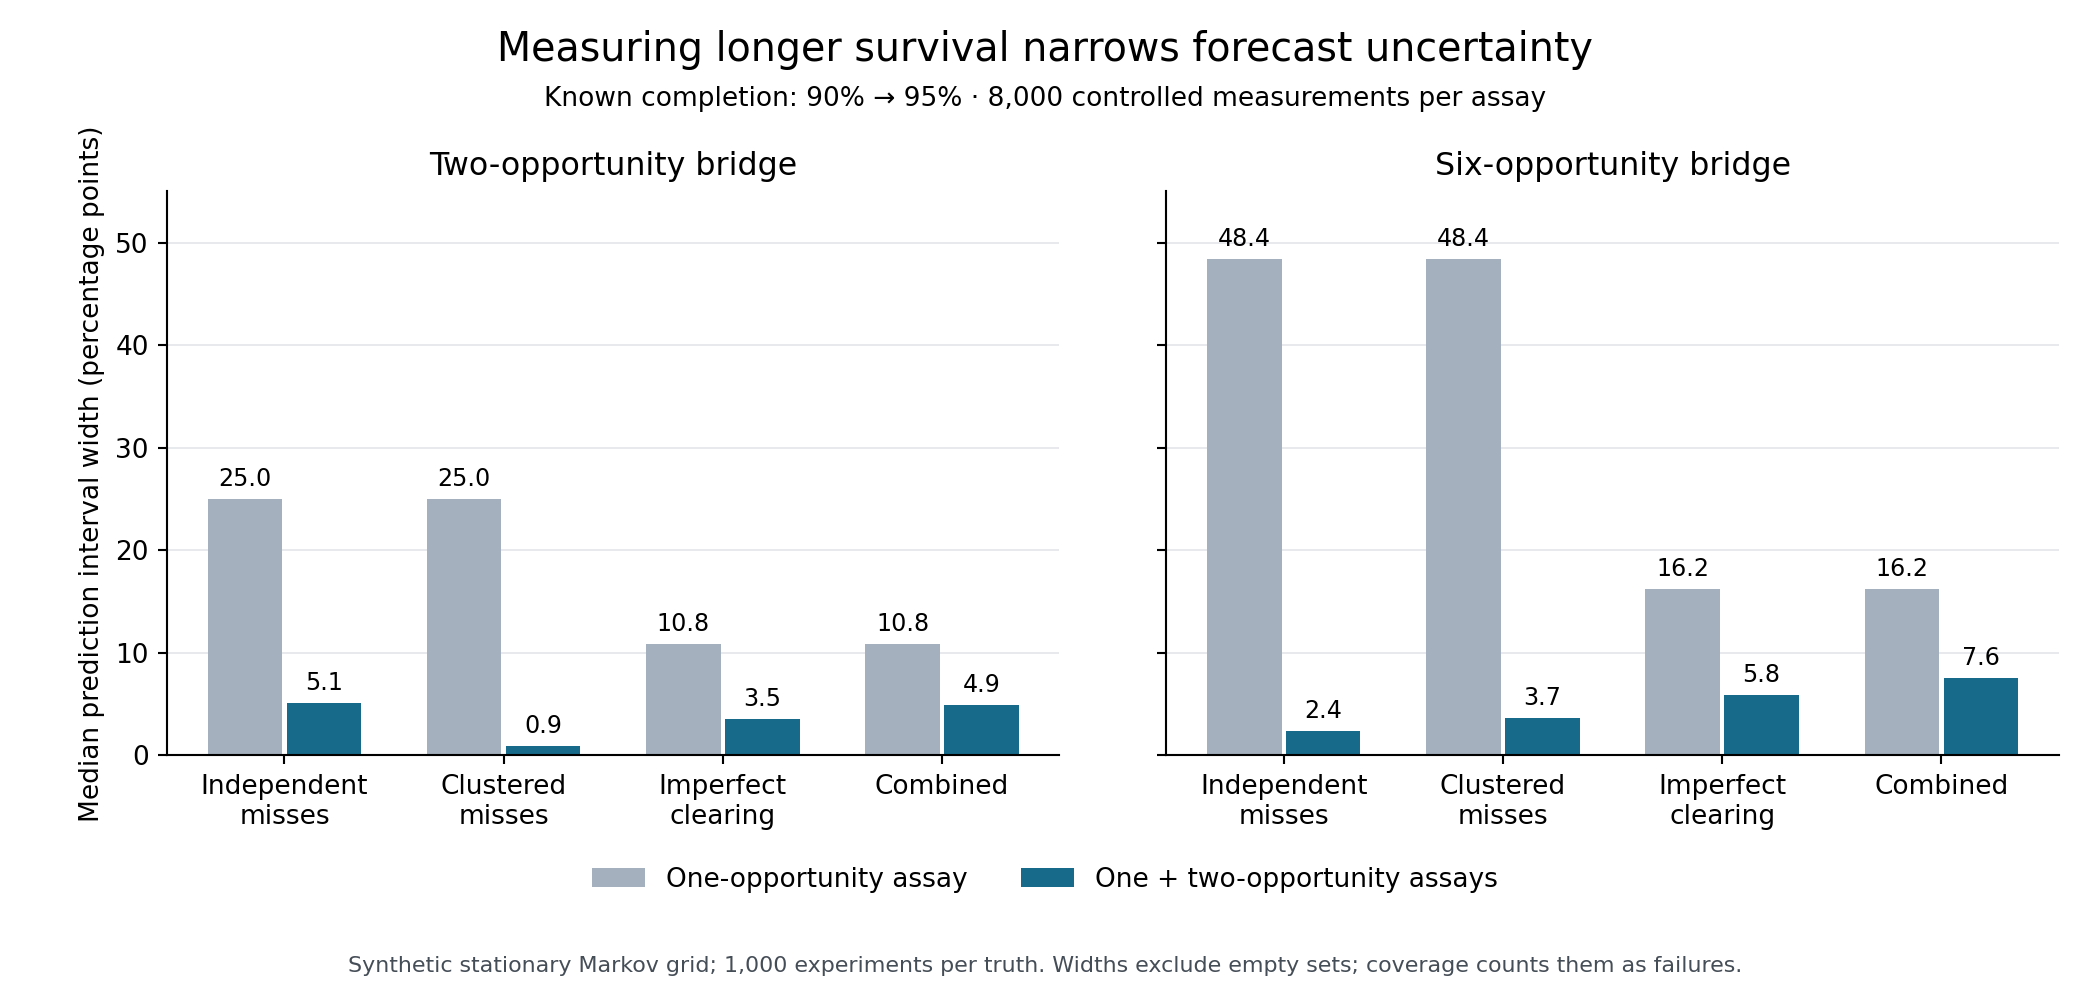
\includegraphics[width=.92\linewidth]{figures/uncertainty_contraction.png}}{\fbox{\parbox{.85\linewidth}{\small The finite-grid contraction figure is archived with the measurement study; the text and Table~\ref{tab:uq-cont} give the plotted quantities.}}}
\caption{Finite-grid measurement study: median projected interval widths for the held-out targets with $q_1$ only and with $q_1$ and $q_2$, by truth and sample size (1,000 repeated synthetic experiments per cell). Synthetic controlled assays with known $h$; conditional on the stationary first-order Markov family.}\label{fig:uq-grid}
\end{figure}

\paragraph{Continuous $k=2$ bounds (post hoc).} The grid understates widths.
Reanalysis of saved .90$\to$.95 measurements removed the grid restriction.
For fixed $e$, the survival ratio is fractional-linear in $\rho$, so extremes
occur at feasible endpoints. Assay constraints give one feasible $e$ interval;
prevention is nondecreasing in $e$ along each clipped $\rho$ boundary, so its
extremes occur at that interval's ends. This argument holds for
$0<h_0<h_1<1$ in this family.

Directed-rounding 60-digit arithmetic resolved all 24,000 confidence sets,
with enclosures at most $10^{-58}$ wide; independent 100-digit calculations
verified all 47,684 extrema and 158 empty-set decisions. This certifies the
optimization given supplied limits, not the full statistical pipeline:
Clopper--Pearson quantiles are floating point, widened by $3\times10^{-12}$.
A verification-only $10^{-90}$ comparison tolerance repaired roundoff near a
point certificate; the solver and outputs did not change.

\begin{table}[htbp]\centering\footnotesize
\caption{Continuous $k=2$ bounds (.90$\to$.95): median interval width (percentage points) with $q_1$ only and with $q_1$ and $q_2$, empty joint sets per 1,000 experiments, and single-target coverage at $n=8{,}000$. Empty sets count as coverage failures. Coverage here concerns one $k=2$ target and is not comparable with the six-target simultaneous coverage above.}\label{tab:uq-cont}
\begin{tabular}{lrrrrr}\toprule
Truth & Measurements per assay & $q_1$ only & $q_1+q_2$ & Empty joint sets & Coverage ($n=8{,}000$)\\\midrule
Independent & 500 & 25.71 & 19.28 & 15 & \\
 & 2,000 & 25.16 & 11.50 & 16 & \\
 & 8,000 & 25.04 & 6.27 & 22 & 95.2\%\\
Clustered & 500 & 25.71 & 5.68 & 14 & \\
 & 2,000 & 25.16 & 2.45 & 10 & \\
 & 8,000 & 25.03 & 1.13 & 15 & 97.0\%\\
Imperfect & 500 & 19.02 & 18.35 & 1 & \\
 & 2,000 & 14.06 & 10.51 & 1 & \\
 & 8,000 & 11.45 & 5.71 & 1 & 97.5\%\\
Combined & 500 & 19.01 & 18.97 & 0 & \\
 & 2,000 & 14.07 & 12.98 & 0 & \\
 & 8,000 & 11.45 & 6.69 & 0 & 99.8\%\\
\bottomrule\end{tabular}
\end{table}

Table~\ref{tab:uq-cont} gives continuous widths. Every defined grid interval
lies within its continuous counterpart. There were 95 empty continuous joint
sets versus 110 grid sets; all 15 newly feasible sets were retained.
With perfect clearing, the roughly 25-point $q_1$-only width reflects the assumed
$\rho\in[0,1]$ support ($F_2$ ranges 75--50\%), rather than data precision.
Small samples give little gain for imperfect and combined truths.
Six-opportunity results remain grid-conditional (Fig.~\ref{fig:uq-k6}).

\begin{figure}[htbp]\centering
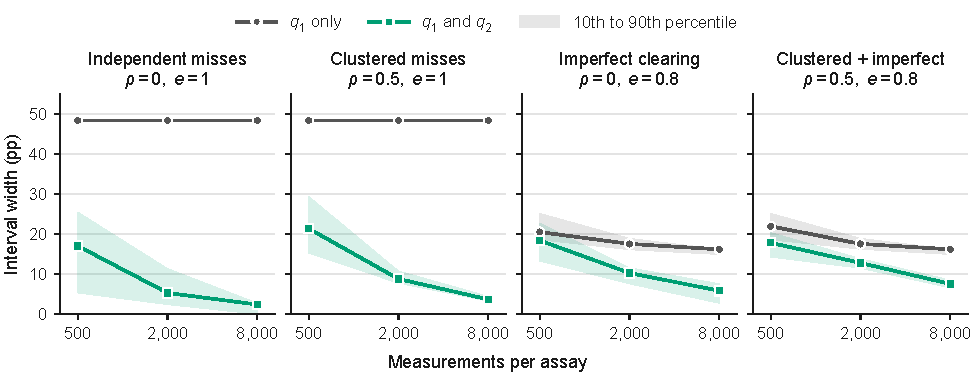
\includegraphics[width=\linewidth]{figures/fig_uq_k6.pdf}
\caption{Six-opportunity bridges: median width of the projected interval for prevention when completion rises from 90\% to 95\% ($h_1=.950$ target), conditional on the finite 4,141-point grid, which can understate widths (it does so for $k=2$). Grey: $q_1$ only; green: $q_1$ and $q_2$; bands, 10th to 90th percentiles over 1,000 experiments per point; empty joint sets (110 of 12,000) excluded from widths and counted as coverage failures.}\label{fig:uq-k6}
\end{figure}

\begin{figure}[htbp]\centering
\IfFileExists{figures/continuous_uncertainty.png}{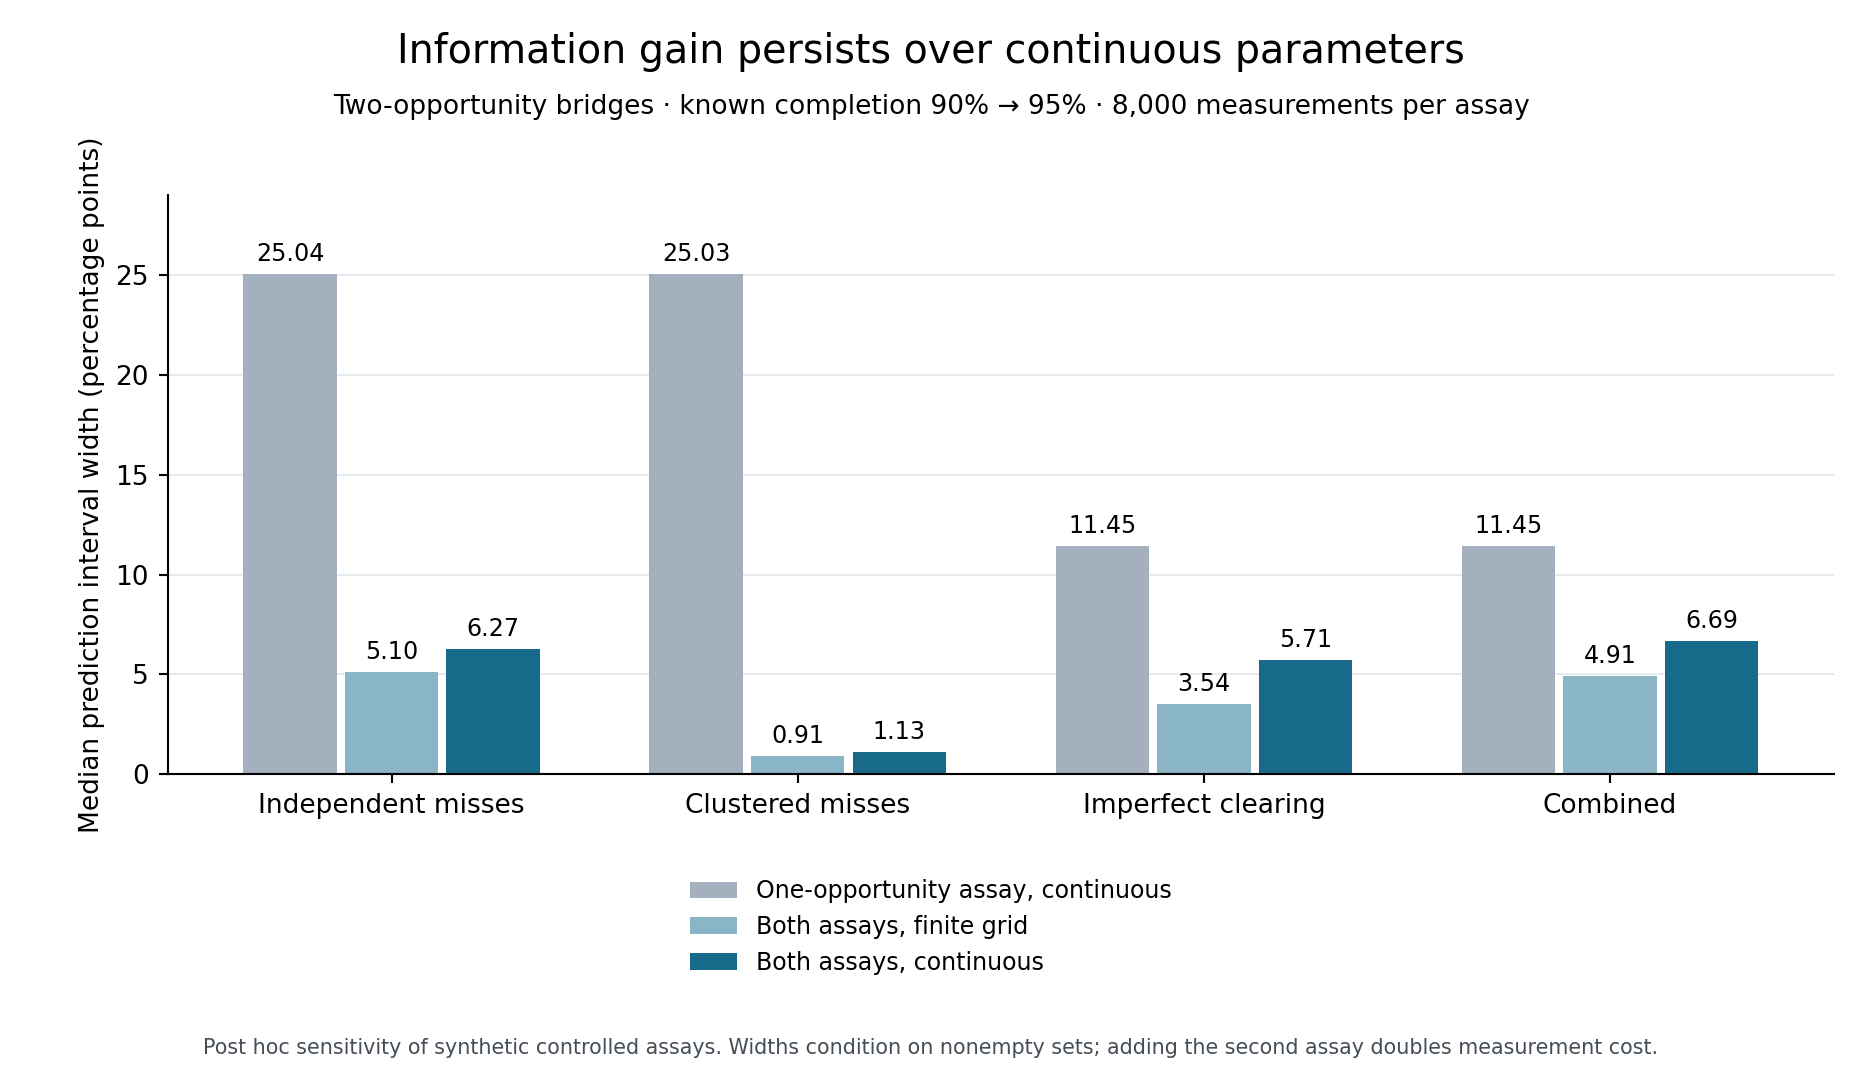
\includegraphics[width=.92\linewidth]{figures/continuous_uncertainty.png}}{\fbox{\parbox{.85\linewidth}{\small The continuous-bounds figure is archived with the measurement study; Table~\ref{tab:uq-cont} gives every plotted median.}}}
\caption{Continuous versus finite-grid $k=2$ interval widths for the same saved measurements (post hoc sensitivity; no new draws).}\label{fig:uq-cont}
\end{figure}

\paragraph{Prespecified non-Markov stress test.} The protocol also fixed a
non-Markov alternative with the same $h$, $q_1$ and $q_2$ as the combined truth at
every $h$, including the policy values. At each arm an episode-level completion
propensity $H$ equals $(1-\rho)h$ with probability $w=(1-h)/(1-h+\rho h)$ and 1
otherwise, with $\rho=.5$, $e=.8$, and completions independent given $H$. Then
$\E[H]=h$ and $\mathrm{Var}(H)=\rho h(1-h)$, so $q_1$ and $q_2$ match the Markov
model exactly, while
$q_k=w(1-e(1-\rho)h)^k+(1-w)(1-e)^k$ generally differs for $k\ge3$. Its $k=2$
prevention is identical, but at $h=.95$ its $k=6$ prevention is 56.42\% against
58.73\% in the matched Markov model. Reusing the combined truth's assay counts
(their distribution is identical), the Markov-projected $k=6$ intervals included
the alternative truth in only 86.8\% of experiments at $n=8{,}000$ (Monte Carlo
95\% interval [84.54, 88.84]); at smaller $n$ the wider intervals covered it
more often. There is no nominal coverage promise for this alternative, and the
figure is not an estimated clinical misspecification rate. Better measurement
can therefore produce narrower, confidently model-dependent predictions unless
the dependence assumption is also assessed.

\paragraph{Projection code check.} The widths above are for isolated bridges.
To project saved assay limits onto an ICU limit surface, each experiment's
feasible $e$ follows from the $q_1$ interval and, at each $e$, the feasible
$\rho$ from the $q_2$ interval; extremes are taken over 81 values of $e$ and 61
of $\rho$. Applied to the isolated bridge, this code reproduces the certified
continuous widths (Table~\ref{tab:icuproj}). An earlier surrogate projection
through a renewal-plus-residual surrogate surface is superseded by the
prespecified projection through the computed coefficient grid below; the
surrogate appears only in the protocol-specified comparison column of
Table~\ref{tab:extension-projection}.

\begin{table}[htbp]\centering\footnotesize
\caption{Median interval widths (percentage points) at 8,000 observations per assay for the isolated two-opportunity bridge: certified continuous extrema, and the discretized projection code as a check. ICU projections are in Table~\ref{tab:extension-projection}.}\label{tab:icuproj}
\begin{tabular}{lrrr}\toprule
Truth & $q_1$ only & $q_1+q_2$ & $q_1+q_2$ (check)\\\midrule
\tabinput{supplement_numbers/tab_icu_projection.tex}
\bottomrule\end{tabular}
\end{table}

\paragraph{ICU grid projection (prespecified extension).}
The extension protocol reused the saved 8,000-per-assay limits, replacing the
surrogate with bilinear interpolation of 132 computed ICU limits on
$\rho\in[0,.95]$, $e\in[.5,1]$. Search used 81 efficacy slices and 61
correlation points per nonempty slice. Sets outside the domain were excluded,
without clipping or extrapolation; none occurred. An independent analytic check
confirmed all 4,000 classifications. Empty and retained sets and conditional
median widths appear in Table~\ref{tab:extension-projection}; the superseded
surrogate is shown on those same sets only as the declared comparison.

The protocol's term ``exact ICU projection'' overstates the calculation.
It interpolates sampled-history coefficients and discretizes feasible sets,
without propagating background uncertainty or certifying continuous extrema.
Ten separately computed crossing nodes gave post hoc discrepancies up to .656
points in $F^*$, not a global error bound or an interval-width bound.
The isolated-bridge certificate and coverage guarantee do not transfer to this
projection. No $q_1$-only ICU projection was computed, so these widths cannot
establish ICU narrowing from adding $q_2$; the combined joint width 11.62 points
is close to the isolated $q_1$-only width 11.4 points.

\begin{table}[htbp]\centering\footnotesize
\caption{Joint-assay ICU projection at 8,000 measurements per assay, 1,000 experiments per truth. Median widths (percentage points) are conditional on retained sets. The coefficient-grid column is interpolated and discretized, with no numerical error bound; the superseded surrogate column, on the same sets, is the protocol-specified comparison only.}\label{tab:extension-projection}
\begin{tabular}{lrrrrr}\toprule
Truth & Coefficient grid & Surrogate & Retained & Empty & Outside domain\\\midrule
\tabinput{supplement_numbers/tab_extension_projection.tex}
\bottomrule\end{tabular}
\end{table}


\paragraph{Verification and limits.} Independent code reproduced all random
counts and defined bounds (285,924 endpoint comparisons; maximum discrepancy
$2.45\times10^{-15}$); it followed results and was not blind. A separate
summary check passed 834 assertions. These forecasts require known $h$,
independently initialized assays, stationary first-order Markov completion,
homogeneous clearing and unchanged $\rho,e$ under policy. They omit measurement
error in $h$ and full-ICU finite-$p$, calibration and workflow uncertainty.
Natural episodes can select completion states in practice, although they do not
in this model (Table~\ref{tab:face}). Clinical feasibility of these assays is
unestablished. Individual completion streams plus technique or culture audits
could instead estimate the parameters; lag-two autocorrelation distinguishes
the Markov law ($\rho^2$) from the non-Markov mixture ($\rho$).

\section{Stability diagnostics and platform notes}\label{sec:s-stability}
These finite-window and bank diagnostics can reveal instability; flat-looking
rates or intervals that include zero do not prove stationarity, sufficient warmup
or equivalence. They are multiple unadjusted checks.

\paragraph{Observation halves.} Tables~\ref{tab:halves} and
\ref{tab:alt-halves} compare first and last 28-day rates. Original imperfect
control rates fell (200,000-draw change interval $[\mn.64,\mn.08]$), while
the inherited-clock independent $p=1$ control rose. Other original control
changes were unresolved. Alternative halves were computed post hoc from daily
blocks (20,000 whole-seed draws, seed 20261023); its controls were stable-looking,
but imperfect policy rates fell. These are finite-window diagnostics, not
stationarity tests.

\begin{table}[htbp]\centering\footnotesize
\caption{Observation-half diagnostics (alternative workflow, post hoc): first-to-last 28-day rate per 1,000 patient-days and a descriptive 95\% interval for last minus first.}\label{tab:alt-halves}
\begin{tabular}{lrrrr}\toprule
Profile & Control & Change [95\%] & Policy & Change [95\%]\\\midrule
\tabinput{supplement_numbers/tab_alt_halves.tex}
\bottomrule\end{tabular}
\end{table}

{\footnotesize\setlength{\tabcolsep}{3pt}
\begin{longtable}{>{\raggedright\arraybackslash}p{.34\linewidth}>{\raggedright\arraybackslash}p{.29\linewidth}>{\raggedright\arraybackslash}p{.29\linewidth}}
\caption{Observation-half diagnostics (original workflow): first-to-last 28-day rate per 1,000 patient-days and a descriptive 95\% interval for last minus first. All intervals have zero undefined draws.}\label{tab:halves}\\
\toprule
Condition & Control first/last; change interval & Policy first/last; change interval\\\midrule\endfirsthead
Condition & Control first/last; change interval & Policy first/last; change interval\\\midrule\endhead
Care-zone: independent (old 512) & $2.82\to 2.84$\newline $[-0.28, 0.33]$ & $0.94\to 0.90$\newline $[-0.19, 0.12]$\\
Care-zone: clustered misses (old 512) & $2.73\to 2.64$\newline $[-0.37, 0.17]$ & $1.18\to 1.19$\newline $[-0.15, 0.18]$\\
Care-zone: imperfect clearing (old 512) & $2.98\to 2.62$\newline $[-0.64, -0.084]$ & $2.08\to 2.02$\newline $[-0.30, 0.18]$\\
Surface-disabled: independent & $0.72\to 0.67$\newline $[-0.17, 0.074]$ & $0.17\to 0.15$\newline $[-0.081, 0.029]$\\
Surface-disabled: clustered misses & $1.45\to 1.37$\newline $[-0.25, 0.091]$ & $0.72\to 0.66$\newline $[-0.18, 0.060]$\\
Surface-disabled: imperfect clearing & $1.70\to 1.62$\newline $[-0.29, 0.11]$ & $1.19\to 1.22$\newline $[-0.13, 0.18]$\\
Independent: upper (matched 256) & $6.92\to 7.66$\newline $[-0.16, 1.65]$ & $2.04\to 2.18$\newline $[-0.28, 0.56]$\\
Independent: center (matched 256) & $2.70\to 2.85$\newline $[-0.28, 0.58]$ & $0.90\to 0.97$\newline $[-0.16, 0.30]$\\
Inherited clock: clustered misses & $3.04\to 3.14$\newline $[-0.23, 0.44]$ & $0.87\to 0.85$\newline $[-0.17, 0.12]$\\
Inherited clock: imperfect clearing & $2.92\to 2.78$\newline $[-0.45, 0.19]$ & $1.09\to 0.96$\newline $[-0.30, 0.040]$\\
Inherited clock: independent boundary & $1.58\to 1.82$\newline $[0.010, 0.47]$ & $0.026\to 0.031$\newline $[-0.017, 0.029]$\\
\bottomrule\end{longtable}
}

\paragraph{Seed banks.} Every study used two disjoint seed banks. In the original
holdout, bank B minus bank A differences in $F$ were $\mn3.1$ [$\mn9.8$, 3.6],
$\mn1.3$ [$\mn8.7$, 6.0] and $+2.7$ [$\mn7.9$, 13.2] percentage points
(independent, clustered, imperfect). In the environmental comparison one
environment-disabled condition ($p=.081$) differed between banks by 17.0 [2.3,
33.0] points; the other five conditions' intervals included zero. Both banks were
kept, as declared. Table~\ref{tab:banks} gives point diagnostics for the
follow-up. In the coefficient studies the bank B minus bank A difference in every
primary limit was at most 0.002 percentage points in either workflow.

{\footnotesize\setlength{\tabcolsep}{3pt}
\begin{longtable}{>{\raggedright\arraybackslash}p{.42\linewidth}rrr}
\caption{A/B bank point diagnostics of the opportunity-rule follow-up: control rates per 1,000 patient-days and prevention (\%). Not formal between-bank equivalence tests. Matched upper/center banks contain 128 seeds each; full/fresh conditions 256 each.}\label{tab:banks}\\
\toprule
Condition & A/B seeds & Control A/B & $F$ A/B (\%)\\\midrule\endfirsthead
Condition & A/B seeds & Control A/B & $F$ A/B (\%)\\\midrule\endhead
Care-zone: independent (old 512) & 256/256 & 2.89/2.77 & 69.1/66.0\\
Care-zone: clustered misses (old 512) & 256/256 & 2.72/2.65 & 56.5/55.2\\
Care-zone: imperfect clearing (old 512) & 256/256 & 2.87/2.73 & 25.7/28.3\\
Surface-disabled: independent & 256/256 & 0.67/0.72 & 74.5/79.9\\
Surface-disabled: clustered misses & 256/256 & 1.44/1.39 & 48.2/54.6\\
Surface-disabled: imperfect clearing & 256/256 & 1.56/1.76 & 22.9/31.7\\
Independent: upper (matched 256) & 128/128 & 7.08/7.50 & 69.1/72.8\\
Independent: center (matched 256) & 128/128 & 2.91/2.64 & 69.2/63.1\\
Inherited clock: clustered misses & 256/256 & 3.07/3.11 & 73.1/71.1\\
Inherited clock: imperfect clearing & 256/256 & 2.74/2.96 & 60.5/67.2\\
Inherited clock: independent boundary & 256/256 & 1.67/1.72 & 98.1/98.5\\
\bottomrule\end{longtable}
}

\paragraph{Weekly control trajectories.} The saved original-holdout trajectories
were binned by week across the 90 warmup and 56 observation days, pooling counts
and patient-days within each bin before division (Fig.~\ref{fig:weekly},
Table~\ref{tab:weekly}). Rates rose during the first four weeks of warmup and
then varied between about 2.3 and 3.3 with no visible trend. Week 13 [84, 91)
spans the day-90 boundary and the final bin [140, 146) has six days. Intervals are
descriptive whole-seed bootstrap intervals (50,000 draws, seed 20261010). The
bank-specific weekly tables are archived in the repository.

\begin{figure}[htbp]\centering
\IfFileExists{figures/weekly_control.png}{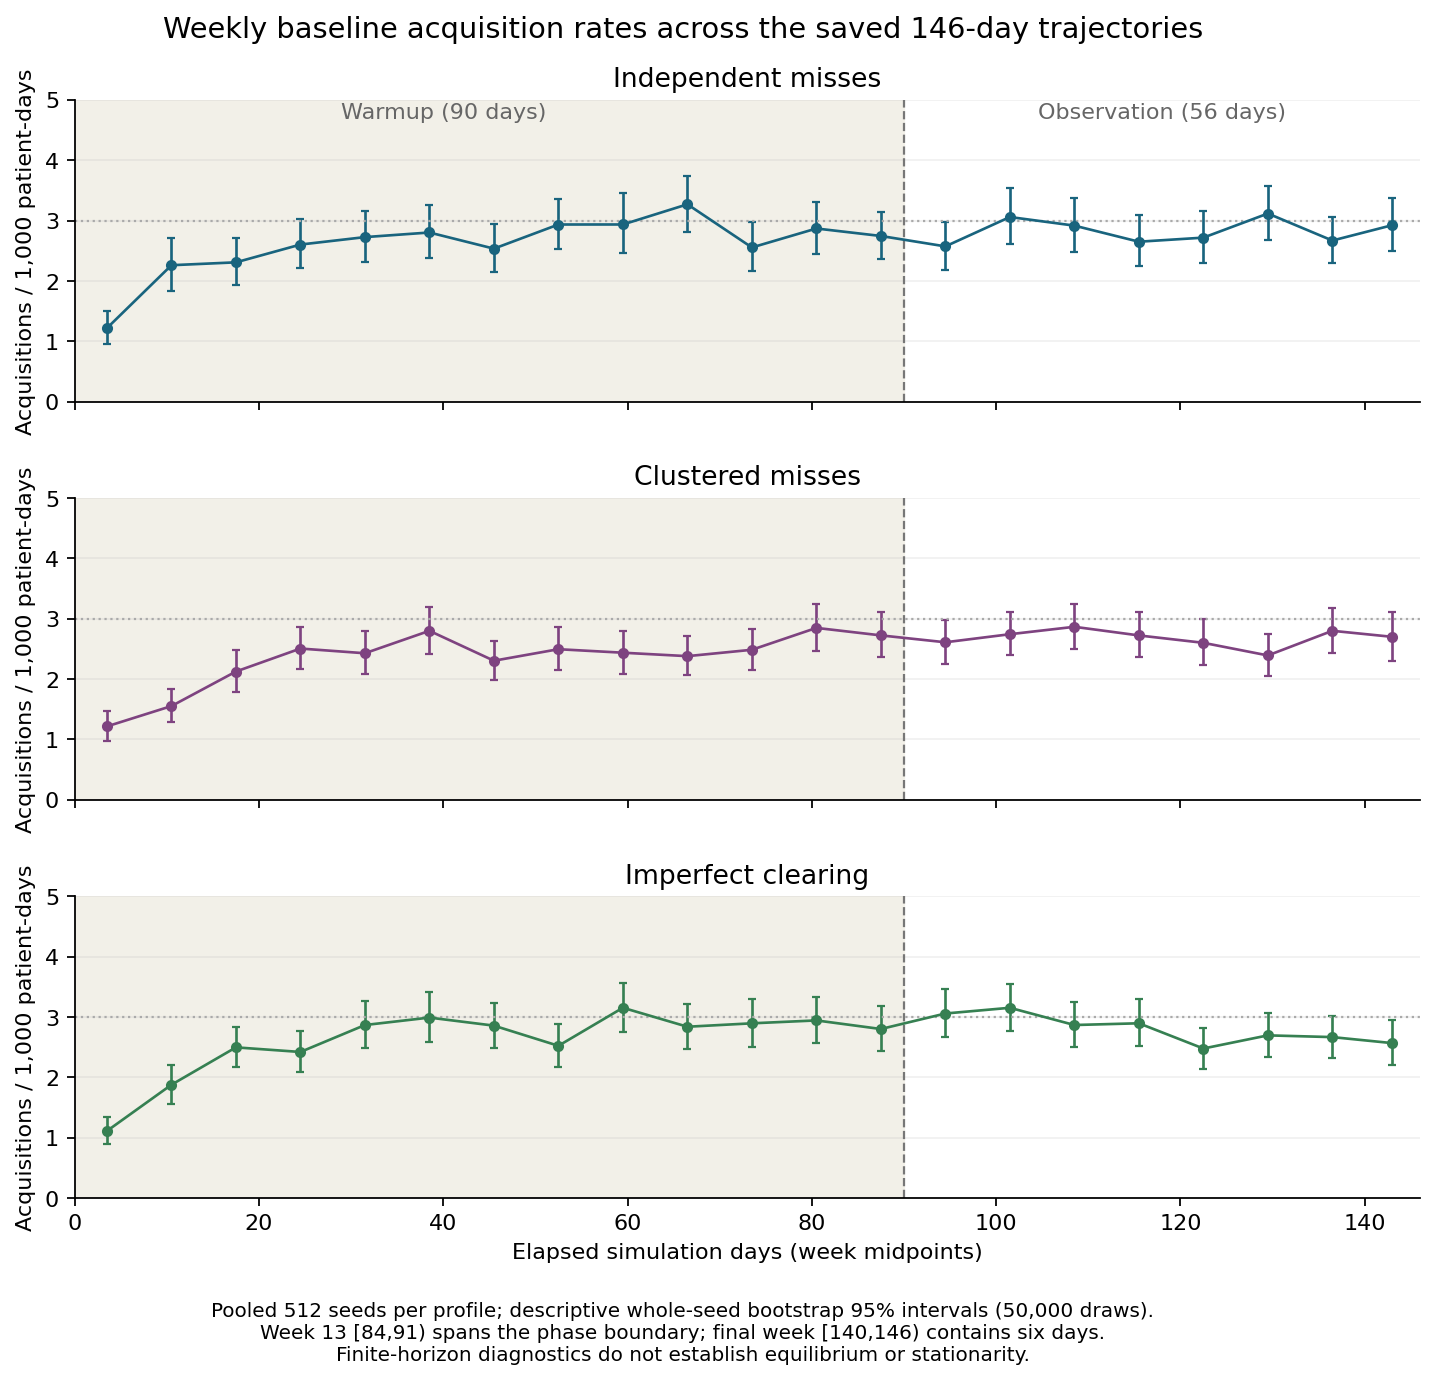
\includegraphics[width=.9\linewidth]{figures/weekly_control.png}}{\fbox{\parbox{.85\linewidth}{\small The weekly-control figure is archived with the reproducible package; Table~\ref{tab:weekly} gives every plotted estimate and interval.}}}
\caption{Weekly control acquisition rates in the original holdout (512 seeds per profile; descriptive whole-seed bootstrap 95\% intervals). Week 13 spans the day-90 boundary; the final bin has six days. The figure describes the saved finite horizon and does not establish equilibrium.}\label{fig:weekly}
\end{figure}

{\footnotesize\setlength{\tabcolsep}{3pt}
\begin{longtable}{>{\raggedright\arraybackslash}p{.055\linewidth}>{\raggedright\arraybackslash}p{.09\linewidth}>{\raggedright\arraybackslash}p{.11\linewidth}>{\raggedright\arraybackslash}p{.205\linewidth}>{\raggedright\arraybackslash}p{.205\linewidth}>{\raggedright\arraybackslash}p{.205\linewidth}}
\caption{Weekly baseline rates per 1,000 patient-days, original holdout, banks pooled.}\label{tab:weekly}\\
\toprule
Week & Days & Phase & Independent [95\%] & Clustered misses [95\%] & Imperfect clearing [95\%]\\
\midrule\endfirsthead
Week & Days & Phase & Independent [95\%] & Clustered misses [95\%] & Imperfect clearing [95\%]\\
\midrule\endhead
1 & [0,7) & warmup & 1.22 [0.95, 1.50] & 1.22 [0.98, 1.46] & 1.11 [0.89, 1.35]\\
2 & [7,14) & warmup & 2.26 [1.84, 2.71] & 1.55 [1.29, 1.83] & 1.88 [1.55, 2.21]\\
3 & [14,21) & warmup & 2.31 [1.94, 2.71] & 2.13 [1.79, 2.49] & 2.50 [2.16, 2.84]\\
4 & [21,28) & warmup & 2.60 [2.21, 3.02] & 2.51 [2.16, 2.87] & 2.42 [2.09, 2.76]\\
5 & [28,35) & warmup & 2.73 [2.32, 3.16] & 2.43 [2.09, 2.79] & 2.87 [2.49, 3.26]\\
6 & [35,42) & warmup & 2.80 [2.38, 3.26] & 2.80 [2.42, 3.19] & 2.99 [2.59, 3.42]\\
7 & [42,49) & warmup & 2.53 [2.14, 2.94] & 2.30 [1.98, 2.64] & 2.86 [2.49, 3.24]\\
8 & [49,56) & warmup & 2.93 [2.52, 3.36] & 2.50 [2.14, 2.87] & 2.52 [2.18, 2.88]\\
9 & [56,63) & warmup & 2.93 [2.47, 3.45] & 2.44 [2.09, 2.80] & 3.15 [2.75, 3.56]\\
10 & [63,70) & warmup & 3.27 [2.81, 3.74] & 2.38 [2.07, 2.71] & 2.84 [2.48, 3.22]\\
11 & [70,77) & warmup & 2.55 [2.16, 2.97] & 2.49 [2.14, 2.84] & 2.90 [2.51, 3.31]\\
12 & [77,84) & warmup & 2.87 [2.45, 3.31] & 2.85 [2.47, 3.25] & 2.94 [2.57, 3.33]\\
13 & [84,91) & mixed & 2.74 [2.36, 3.14] & 2.72 [2.36, 3.11] & 2.80 [2.43, 3.18]\\
14 & [91,98) & observation & 2.57 [2.18, 2.98] & 2.61 [2.26, 2.98] & 3.06 [2.67, 3.46]\\
15 & [98,105) & observation & 3.06 [2.61, 3.54] & 2.74 [2.39, 3.11] & 3.15 [2.77, 3.55]\\
16 & [105,112) & observation & 2.92 [2.49, 3.37] & 2.87 [2.50, 3.25] & 2.87 [2.50, 3.26]\\
17 & [112,119) & observation & 2.65 [2.24, 3.09] & 2.72 [2.36, 3.12] & 2.90 [2.52, 3.30]\\
18 & [119,126) & observation & 2.72 [2.30, 3.16] & 2.60 [2.23, 2.99] & 2.48 [2.15, 2.82]\\
19 & [126,133) & observation & 3.12 [2.68, 3.57] & 2.39 [2.05, 2.75] & 2.70 [2.34, 3.07]\\
20 & [133,140) & observation & 2.67 [2.30, 3.06] & 2.80 [2.44, 3.18] & 2.67 [2.33, 3.02]\\
21 & [140,146) & observation & 2.92 [2.49, 3.38] & 2.70 [2.30, 3.11] & 2.57 [2.20, 2.96]\\
\bottomrule
\end{longtable}
}

\paragraph{Execution platforms.} The original holdout (1,344 Linux-cluster and 192
local macOS paired jobs) and the environmental comparison (2,688 and 384) mixed
two platforms with identical scientific sources and package versions (Linux,
Python 3.12.3; macOS arm64, Python 3.12.2; NumPy 1.26.4 and Mesa 1.2.1 on both).
All 3,072 alternative-workflow records ran on one Linux host with one pinned
build. The common-baseline analysis uses an independent lower bank of 64 macOS
and 192 Linux records, with all upper and sensitivity records on Linux. Scientific source
hashes and package versions agree, but exact cross-platform recomputation of those
records was not verified, so platform effects could affect marginal estimates,
not merely pairing efficiency; the intervals condition on the recorded execution
mixture. A Linux-only subset of 192 pairs gave 66.6\% [61.3, 72.0] against
66.7\% in the primary analysis (Section~\ref{sec:s-common}); this changes the seed
subset as well as the platform mixture. The alternative-workflow coefficient
study ran on macOS (Section~\ref{sec:s-repro}). The original-workflow coefficient
backgrounds were produced on both platforms (38 partitions, 32 cluster and 6
local). The measurement study is a small local synthetic benchmark on macOS.

\section{Reproducibility}\label{sec:s-repro}
\paragraph{Archives.} Frozen configurations, seed lists, source code, analysis
scripts and records are preserved with checksums: the earlier 8,576 records, the
5,760 records of the opportunity-rule follow-up (whose analysis reuses the 1,536
original holdout records, not counted again), the 3,072 alternative-workflow
records, the 256 alternative-workflow coefficient records and the 256
original-workflow coefficient-extension records. Paired branches
are not separate records. The common-baseline analysis, the addenda and the
measurement study add no ICU simulation records. Earlier exploratory studies
remain archived, including failed fits and a 21-day calibration study
whose fresh validation runs had lower baseline acquisitions than its training
runs; an audit found no configuration or implementation difference, and no cause
was identified. Its 21-day records enter no analysis reported here, and every
later study used two disjoint, equally weighted seed banks
(Section~\ref{sec:s-stability}). Clinical spreadsheets from the original project
are not public; every model input derived from them is encoded in the preserved
configuration, and none is needed to reproduce any result.

\paragraph{Repository records and availability.}
The code, synthetic data and technical execution extracts are available at
\url{https://github.com/ndandnd/icu-hygiene-calibration} (release v1.0.2), under
\path{execution_records/}.
Its \path{INDEX.md} maps the extracts to the original sections. It includes
execution amendments, runtime details, replay checks, seed lists and summary
hashes. This standalone report preserves the detailed scientific tables and execution
record. The main article and its core supplementary PDF are distributed with
the journal submission rather than this repository.
Dataset descriptions and reproduction instructions are in the repository;
no public DOI is claimed here.

Linux production used Python 3.12.3; local macOS runs used Python 3.12.2,
with NumPy 1.26.4 and Mesa 1.2.1 on both. Cross-platform evidence and its limits
are reported in Sections~\ref{sec:s-alt-verification} and
\ref{sec:s-stability}. The alternative-workflow coefficient study was local;
original-mode recomputation covered five cluster-origin and five local-origin seeds,
but alternative mode was not checked across platforms. The synthetic
measurement study used macOS and SciPy 1.13.1.

Scientific tables remain generated from preserved inputs by
\path{../supplement_numbers/make_supplement_tables.py} and
\path{../supplement_numbers/make_extension_tables.py}. Their number-provenance maps
bind displayed values to source fields, rounding and input/output hashes.
Neither script was rerun for this edit.

\section{Directional transfer and bounded worker heterogeneity}\label{sec:s-directional}
This post hoc analysis uses the saved coefficient histories only. It adds no
transmission simulation, background seed, bootstrap draw or clinical input.
The stress ranges below were written down before reweighted outcomes were
computed; the original aggregate outcomes were already known.

\paragraph{Global asymmetry and the limit.}
The common finite-$p$ transfer parameter is a structural simplification. Its
equality across directions is unnecessary for the leading hand-bridge ratio.
Under the assumptions of Proposition~\ref{prop:icu}, let patient-to-hand,
hand-to-patient, hand-to-site and site-to-hand probabilities be respectively
$\epsilon a,\epsilon b,\epsilon c,\epsilon d$, times the existing contact
weights, with fixed bounded constants and $a,b>0$. For sufficiently small
$\epsilon$ these are valid probabilities. Exactly two successful transmissions
can produce an acquisition only by imported patient--hand--susceptible patient
transfer. Hence
\[
\E C_h=\epsilon^2ab\bar K_h+O(\epsilon^3),\qquad
F\longrightarrow1-\bar K_{h_1}/\bar K_{h_0}.
\]
Both coefficients acquire the same factor $ab$, which cancels. With initially
clean sites, an environmental chain additionally needs hand-to-site deposition
and site-to-hand pickup: its first possible contribution is fourth order when
all four directions scale with $\epsilon$. Cubic corrections need not be
environmental. If surface exchange instead stays of order one, this is a
different asymptotic regime. None of these identities validates directional
robustness at the finite probabilities used in the simulations.

\paragraph{A conditional reweighting bound.}
Let bridge types have nonnegative baseline shares $w_j$ summing to one and
survival ratios $r_j=s_{1j}/s_{0j}$, with $s_{0j}>0$. Suppose altered pickup and
transfer weights multiply bridge $j$ by $t_j\in[m,M]$, where $0<m\le M$,
identically in both hygiene arms. Then
\[
F^*(t)=1-\frac{\sum_jw_jt_jr_j}{\sum_jw_jt_j},\qquad
\left|F^*(t)-F^*(1)\right|
\le (r_{\max}-r_{\min})
       \frac{\sqrt M-\sqrt m}{\sqrt M+\sqrt m}.
\]
This is a convenient corollary of bounded reweighting, not a new general
probability theorem. To prove it, put $\mu=\sum_jw_jt_j$ and
$u_j=w_jt_j/\mu$. A bounded mean changes by at most its range times total
variation. Convexity of $|t-\mu|$ on $[m,M]$ gives
\[
\tfrac12\sum_j|u_j-w_j|
\le\frac{(M-\mu)(\mu-m)}{\mu(M-m)}
\le\frac{\sqrt M-\sqrt m}{\sqrt M+\sqrt m},
\]
with the last maximum at $\mu=\sqrt{mM}$; $m=M$ follows by continuity.
Two types with endpoint multipliers and endpoint survival ratios attain the
bound over unrestricted spectra. Attainability need not hold for a particular
ICU or for factorized pickup/transfer weights. Types with zero baseline but
positive policy coefficient fall outside this statement.

\paragraph{Saved-data calculation.}
Both workflows retain baseline and policy coefficients by worker in all 256
background records, for each of $(\rho,e)=(0,1),(.5,1),(0,.8),(.5,.8)$.
For each worker $u$, pool these coefficients as $A_u,B_u$ over backgrounds and
compute $F^*(t)=1-\sum_ut_uB_u/\sum_ut_uA_u$. One multiplier applies to the same
worker across seeds and both arms. A worker-specific pickup factor times its
transfer factor can realize this product; varying their ratio alone cancels.
No worker-role interpretation or within-worker contact heterogeneity is inferred.

We optimized the ratio over $t_u\in[1/2,2]$ and $[1/4,4]$, mathematical stress
ranges without empirical or clinical status. Sort $B_u/A_u$ and evaluate the
endpoint assignments at each threshold to obtain the exact fractional-program
extrema. An independent implementation solved the residual-root equations
instead. All 790 bound input hashes, both complete 256-record banks, the original
archived references and all worker sums passed verification. Exact rational
arithmetic treats saved decimal coefficients as inputs; it does not certify the
original coefficient engine's numerical error. The largest relative discrepancy
between summed worker coefficients and recorded totals was below
$4\times10^{-13}$.

\begin{table}[htbp]\centering\small
\caption{Conditional leading-order prevention (\%) under worker reweighting.
Endpoints are rounded outwards to two decimals. These are structural bounds on
saved pooled coefficients, not confidence intervals. The combined profile has
$(\rho,e)=(.5,.8)$.}\label{tab:worker-reweighting}
\begin{tabular}{llrrr}\toprule
Workflow & Profile & Nominal & $t_u\in[1/2,2]$ & $t_u\in[1/4,4]$\\\midrule
\tabinput{addenda/tab_worker_reweighting.tex}
\bottomrule\end{tabular}
\end{table}

All profile rankings retain their signs throughout either box in both workflows:
independent misses, clustered misses, combined, then imperfect clearing.
In particular, clustering lowers prevention with perfect clearing and raises it
at $e=.8$. Subtracting separately optimized profile intervals gives conservative
bounds for contrasts with the same worker multipliers; no jointly sharp contrast
interval is claimed. The bounds condition on these backgrounds and omit their
Monte Carlo uncertainty, finite-transmission feedback, arbitrary contact-specific
heterogeneity and estimation of transfer parameters. They do not establish
matched finite-$p$ baselines or clinical validity.

The plan, mathematical derivation, exact check, input hashes, analysis and
independent recomputation are preserved under
\path{research/referee_perspective_2026-10-24/}. This calculation changes none of
the original studies, failed matching checks or coefficient predictions.


\nocite{austin1999,baek2022,barnes2014,beggs2009,bertsimas2005,chan2026,clopper1934,degeyter2017,grimm2020,kraay2018,madansky1959,manski2003,mitchell2015,spicknall2010,tamer2010,wei2021,who2009,whoguidelines2009}
\bibliographystyle{canonical-technical_report}
\bibliography{references}
\end{document}
